\documentclass[12pt,oneside]{book}

\usepackage[T1]{fontenc}
\usepackage[utf8]{inputenc}
\usepackage{lmodern}
\usepackage[a4paper,margin=1in]{geometry}
\usepackage{setspace}
\usepackage{graphicx}
\usepackage{booktabs}
\usepackage{array}
\usepackage{tabularx}
\usepackage{longtable}
\usepackage{amsmath}
\usepackage{amssymb}
\usepackage{float}
\usepackage{url}
\usepackage{xcolor}
\usepackage[numbers,sort&compress]{natbib}
\usepackage[hidelinks]{hyperref}
\usepackage{caption}

\graphicspath{{figures/}}
\setstretch{1.25}
\captionsetup{font=small,labelfont=bf}
\setcounter{secnumdepth}{3}
\setcounter{tocdepth}{2}

\begin{document}

\begin{titlepage}
  \centering
  {\Large [University Name] \par}
  \vspace{1cm}
  {\large [Faculty or School Name] \par}
  \vspace{2cm}
  {\Huge\bfseries Offline-Capable Guardrail Detection for Jailbreak and Prompt Injection Inputs in Large Language Model Applications\par}
  \vspace{1.5cm}
  {\Large Capstone Thesis\par}
  \vfill
  \begin{tabular}{rl}
    Author: & Lee Rui Da \\
    Student ID: & [Student ID] \\
    Supervisor: & [Supervisor Name] \\
    Programme: & [Programme Name] \\
    Submission Date: & March 2026 \\
  \end{tabular}
  \vfill
\end{titlepage}

\frontmatter
\chapter*{Abstract}
\addcontentsline{toc}{chapter}{Abstract}

Large language model applications often assemble prompts from multiple text sources --- user input, retrieved passages, and attached context --- which makes prompt-layer attacks such as jailbreaks and prompt injection a practical deployment risk. This thesis studies prompt-layer guardrail detection as a binary classification problem over a single text payload. The delivered system is an offline-capable detector with a command-line interface and Python library, exposing an always-available rules baseline and an optional learned LoRA classifier that runs strictly from local artifacts.

Methodologically, the thesis makes a threshold-transfer evaluation protocol central to the analysis. The learned detector is implemented as a parameter-efficient LoRA sequence classifier with a DeBERTa-v3-base backbone, and the final selected run is \texttt{week7\_norm\_only}. A decision threshold of \(\tau = 0.7340\) is calibrated on validation at target false-positive rate (FPR) \(= 1\%\) and then transferred unchanged to held-out splits, avoiding optimistic per-split threshold tuning. Robustness is assessed using reproducible perturbation families that probe common evasion channels: Unicode obfuscation, character-level noise (adv2), and paraphrase-like rewriting.

Empirically, the learned detector achieves strong ranking quality on the main evaluation distribution (\(\mathrm{AUROC}=0.9958\) on \texttt{test\_main}), but the fixed operating point does not transfer stably under shift. At the same transferred threshold, benign FPR rises from \(0.0094\) on validation to \(0.0311\) on \texttt{test\_main}, \(0.5816\) on \texttt{test\_jbb}, and \(0.6403\) on \texttt{test\_main\_adv2}. The main contribution is therefore not a claim of deployment-ready robustness, but an examiner-verifiable demonstration that high AUROC and AUPRC do not guarantee low-FPR deployment behavior under distribution shift. The thesis argues that the threshold should be treated as a monitored policy object, that the rules baseline remains a conservative offline fallback, and that the committed Week~7 locked evaluation pack should be treated as the authoritative source of reported counts, metrics, and figures.

\noindent\textbf{Keywords:} large language models, prompt injection, jailbreak detection, guardrails, threshold calibration, robustness evaluation

\tableofcontents
\listoffigures
\listoftables

\mainmatter
\chapter{Introduction}
\label{ch:introduction}

Large language models (LLMs) are increasingly deployed as components inside larger applications rather than as standalone chat interfaces. Many systems assemble a final model input by combining a user prompt with retrieved passages, application-provided context, or tool outputs. In this setting, natural language becomes a control surface: untrusted strings can influence downstream behavior in ways that resemble injection flaws in traditional software systems. This creates practical risk for instruction takeover, policy bypass, and attempted secret or system-prompt extraction.

This thesis studies prompt-layer guardrail detection. Given an input payload consisting of the user prompt plus any attached context, a detector assigns an attack-likelihood score and decides whether the payload should be flagged as an attack or treated as benign. The implemented system is a CLI-first, offline-capable detector with two runtime backends: a deterministic rules baseline and an optional learned LoRA classifier. Evaluation is grounded in a locked protocol where the decision threshold is learned on validation and transferred unchanged to held-out splits.

Figure~\ref{fig:system_context} situates the detector in the intended application flow. The key scope boundary is that the detector screens text before a downstream LLM call; it does not claim to solve tool sandboxing, permissioning, or full application security.

\begin{figure}[t]
  \centering
  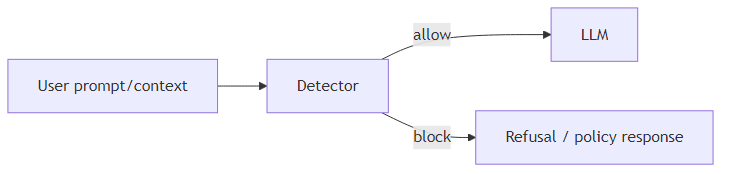
\includegraphics[width=0.9\linewidth]{ch1_system_context.png}
  \caption{System context: the detector screens prompt and context before the downstream LLM call.}
  \label{fig:system_context}
\end{figure}

\section{Background and threat model}

This thesis considers two related prompt-layer threats. A \emph{jailbreak} is a prompt crafted to override policy or instruction hierarchy and induce disallowed behavior. A \emph{prompt injection} is an instruction embedded in text that becomes part of the model input because an application concatenates user prompt and context. In the direct case, the attacker controls the user prompt; in the indirect case, the malicious instruction is embedded in retrieved or attached context \cite{rababah2024sokprompthacking,abdelnabi2023promptinjection}.

The central security concern is that LLM applications often treat all text in the context window as potentially instruction-bearing. When trusted instructions and untrusted content are mixed into one payload, the application may unintentionally expose its instruction boundary to adversarial text. This is the prompt-layer analogue of control-data confusion.

\section{Why low false-positive rate matters}

A detector is only useful if it is operationally tolerable. Excessive blocking of benign prompts creates user friction, hides system capability behind false alarms, and undermines trust in the guardrail itself. For that reason, the evaluation in this thesis is organized around a strict operating-point target of approximately 1\% FPR on validation. This target is a calibration goal, not a guarantee that a single fixed threshold will remain at 1\% under shift.

This framing also clarifies the reporting strategy. Threshold-free metrics such as AUROC and AUPRC summarize ranking quality, but deployments run at a single threshold. The thesis therefore reports both ranking metrics and fixed-threshold metrics: FPR, TPR, and ASR (attack success rate, equal to the attack false-negative rate at the operating threshold).

The resulting evaluation should be read as a threshold-transfer stress study rather than as a direct simulation of production traffic priors. Validation is used to learn the operating point, while the held-out splits are designed to expose shift and robustness failure. That design is appropriate for the thesis question, but it is not equivalent to measuring field performance on a benign-heavy production stream.

\section{Project goals}

The project goals are defined as delivered system and evaluation artifacts:
\begin{enumerate}
  \item Provide an offline-capable detector system with a CLI and Python library for single-prompt and batch scoring.
  \item Calibrate a low-FPR operating threshold on validation and transfer it unchanged to held-out splits.
  \item Produce an examiner-verifiable evidence bundle containing the final protocol, aggregate tables and figures, and sanitized error-case summaries.
\end{enumerate}

\section{Research questions and hypotheses}

The thesis is organized around three research questions:
\begin{itemize}
  \item \textbf{RQ1.} How does a validation-calibrated threshold at FPR = 1\% transfer across held-out splits under distribution shift when applied unchanged?
  \item \textbf{RQ2.} Which perturbation families most degrade low-FPR threshold-transfer stability under fixed operating-point evaluation?
  \item \textbf{RQ3.} How does the project's fully offline rules baseline compare to the optional learned detector under the same runtime interface and evaluation constraints?
\end{itemize}

The corresponding hypotheses are:
\begin{itemize}
  \item \textbf{H1 (threshold drift).} A threshold calibrated on validation at 1\% FPR will drift on at least some held-out splits because calibration is not re-tuned per split.
  \item \textbf{H2 (stress ordering).} adv2-style character perturbations will produce the largest degradation in threshold-transfer stability; Unicode perturbations will mostly affect calibration; rewrite perturbations will be milder on the main distribution.
  \item \textbf{H3 (baseline vs learned).} The rules detector is a viable offline baseline for demos and transparency within the shipped runtime, while the learned detector provides stronger scoring when local artifacts are available.
\end{itemize}

\section{Contributions}

This thesis contributes three distinct outputs, each with a different academic role:
\begin{itemize}
  \item \textbf{Empirical contribution.} The thesis shows that strong threshold-free ranking performance does not preserve a low-FPR operating point under distribution shift. In the locked Week~7 study, the selected run \texttt{week7\_norm\_only} remains strong on the main distribution but exhibits large benign false-positive drift on JBB-style and adv2-style inputs.
  \item \textbf{Methodological contribution.} The thesis adopts a low-FPR threshold-transfer protocol in which the decision threshold is calibrated on validation and transferred unchanged to all held-out splits. This frames guardrail detection as an operating-point evaluation problem rather than a threshold-free leaderboard exercise.
  \item \textbf{Systems contribution.} The project delivers an offline-capable jailbreak and prompt-injection detector with a common runtime interface for a rules baseline and an optional LoRA detector, together with a committed Week~7 locked evaluation pack containing source-of-truth tables, figures, sanitized error cases, and configuration and environment snapshots.
\end{itemize}

\section{Scope and claim boundary}

The scope of this work is deliberately narrow. The detector screens a text payload before the downstream LLM call; it does not provide end-to-end application security guarantees, tool sandboxing, or full application security. The project does not claim robustness beyond the evaluated datasets and perturbation families, and it does not claim production readiness. The original proposal named comparison against external guardrails such as Llama Guard 2, Prompt Guard, and ProtectAI-style detectors; because no runnable local artifacts for those systems were available in the submission environment, the final thesis narrows scope openly to an offline reproducible detector study rather than overstating an undelivered benchmark. The strongest defensible statement is therefore precise: the shipped system and locked Week~7 pack provide explicit evidence of where a low-FPR operating point succeeds, where it drifts, and why that drift matters for deployment.

\section{Thesis roadmap}

Chapter~\ref{ch:related_work} surveys related work on jailbreaks, prompt injection, guardrails, and low-FPR evaluation. Chapter~\ref{ch:method} defines the task, data representation, preprocessing, detectors, metrics, and locked protocol. Chapter~\ref{ch:experiments} reports the final Week~7 experimental results and selection logic. Chapter~\ref{ch:robustness} analyzes robustness and threshold-transfer failure modes. Chapter~\ref{ch:system_demo} documents the system and demo implementation. Chapter~\ref{ch:limitations_ethics} discusses limitations, ethics, and safe deployment posture. Chapter~\ref{ch:conclusion} concludes and outlines future work.


\chapter{Related Work}
\label{ch:related_work}

This chapter situates jailbreak and prompt-injection detection within prior work on LLM security, adversarial text robustness, and practical guardrail evaluation. The literature spans three overlapping threads: attack construction, defense mechanisms, and evaluation methodology. In line with the scope of this thesis, the work focuses on prompt-layer screening: scoring a single text payload that represents the user prompt plus any attached context before it reaches a downstream LLM.

\section{Jailbreak attacks and defenses}

Jailbreaks are prompts crafted to induce policy-violating behavior by manipulating instruction hierarchy, authority cues, or multi-step compliance patterns. Recent surveys organize these methods under broader prompt-hacking taxonomies and emphasize their recurring structure: instruction override, role escalation, and staged compliance scaffolding \cite{rababah2024sokprompthacking}. These surveys are useful because they explain why many jailbreaks share surface cues that can be targeted by rules or detectors, while also showing why attacker adaptation quickly erodes brittle defenses.

Benchmark-style evaluation has become increasingly important. JailbreakBench provides a structured way to assess jailbreak robustness across standardized prompt sets rather than isolated anecdotal prompts \cite{chao2024jailbreakbench}. Automated red-teaming work similarly argues for repeatable attack suites and operational metrics rather than one-off demonstrations \cite{perez2022redteaming}. These developments motivate a detector evaluation protocol that is explicit about operating points and held-out distributions.

Defense work generally falls into three families: model-level alignment and refusal training, inference-time guardrails such as rule filters or safety classifiers, and system-level prompt-architecture mitigations. This thesis contributes to the second category by evaluating two input-side guardrails behind a common score-and-threshold interface: a transparent rules baseline and an optional learned classifier.

\section{Prompt injection and indirect injection}

Prompt injection differs from jailbreaks mainly in where the malicious instruction originates and how it enters the final model input. In direct prompt injection, the attacker places the instruction in the user prompt. In indirect prompt injection, the malicious text is embedded in external content --- retrieved passages, documents, or tool outputs --- that the application later concatenates into the prompt seen by the model \cite{abdelnabi2023promptinjection}. This distinction is especially important for retrieval-augmented and agentic systems because an attacker may never control the user prompt itself.

Related work on prompt extraction and prompt leakage further reinforces the idea that the prompt boundary is a security boundary. Models can be coerced into revealing hidden instructions or system prompts, and the same prompt-layer weaknesses that enable leakage also motivate input-side screening \cite{zhang2023effectivepromptextraction}.

\section{Guardrails and low-FPR evaluation}

Rule-based guardrails remain appealing because they are fast, interpretable, and easy to deploy in constrained environments. They can catch recurrent takeover phrases and obvious system-prompt extraction attempts, but prior work also notes their brittleness under paraphrase and obfuscation \cite{rababah2024sokprompthacking,chao2024jailbreakbench}. Learned detectors, by contrast, can generalize beyond exact strings, but they introduce calibration and distribution-shift risks.

That distinction is why threshold-free metrics are not sufficient. AUROC and AUPRC summarize ranking quality across all thresholds, but deployments operate at one threshold. Work on calibration shows that modern neural networks can be poorly calibrated, meaning a threshold that behaves well on validation may drift under shift \cite{guo2017calibration}. Classical ROC analysis likewise emphasizes that the best threshold depends on the cost structure and the intended operating region \cite{fawcett2006roc}. This thesis therefore adopts a threshold-transfer protocol: select the threshold on validation at a target FPR, then apply it unchanged to held-out splits.

\section{Unicode security and adversarial text perturbations}

Unicode creates multiple evasion channels: fullwidth characters, confusables, combining marks, invisible separators, and bidirectional controls. Unicode normalization and security guidance formalize many of these concerns and motivate canonicalization as a practical hardening step \cite{unicode_uax15,unicode_uts39}. Trojan Source demonstrates how invisible Unicode controls can change interpretation without obvious visual differences, illustrating the wider security relevance of Unicode manipulation \cite{boucher2023trojansource}.

Because attacker behavior is adaptive and hard to sample exhaustively, robustness evaluation often uses controlled perturbation suites. In adversarial machine learning, adversarial examples and robust optimization established the value of systematic stress tests that probe brittleness under targeted transformations \cite{goodfellow2015adversarial,madry2018towards}. In this thesis, Unicode obfuscation, adv2-style character noise, and rewrite-style paraphrase are used as reproducible robustness probes. They do not claim to cover all attacker strategies, but they make distribution-shift and operating-point failure observable.

\begin{table}[t]
\centering
\caption{Threats, evaluated defenses, and common weaknesses.}
\label{tab:threats_defenses}
\scriptsize
\begin{tabularx}{\textwidth}{p{0.16\textwidth}p{0.13\textwidth}p{0.2\textwidth}p{0.2\textwidth}X}
\toprule
Threat / evasion tactic & Typical setting & Representative defenses in prior work & Defenses evaluated in this thesis & Common weaknesses / gaps \\
\midrule
Direct jailbreak prompts & Prompt-only & Alignment and refusal training, safety classifiers, rule filters, structured prompting, red-teaming suites & Rules baseline, learned classifier, low-FPR thresholding & Paraphrase and novel prompt patterns can evade brittle cues; calibration drifts under shift \\
Direct prompt injection & Prompt-only & Same as jailbreak plus instruction-hierarchy enforcement & Same detector interface as jailbreak & Ambiguous boundary between benign discussion and malicious takeover language \\
Indirect prompt injection & RAG / retrieved context & Context separation, trust scoring, retrieval filtering, input scanning & Single-payload scanning over prompt plus context & Malicious instructions can be embedded subtly inside attached context \\
Unicode obfuscation & Any text channel & Normalization, confusable detection, canonicalization & NFKC/category stripping and optional preprocessing & Incomplete coverage; aggressive normalization can distort benign text \\
Character noise (adv2-like) & Any text channel & Robust training, augmentation, character-level models & adv2 stress variants and ablations & Can distort tokenization and move benign mass above a fixed threshold \\
Paraphrase / rewrite & Any text channel & Semantic models, paraphrase-robust training, ensembles & Rewrite stress variants and ablations & Rules are brittle; learned detectors may retain AUROC while drifting at the operating point \\
\bottomrule
\end{tabularx}
\normalsize
\end{table}
\begin{table}[t]
\centering
\caption{Representative prior work compared with the scope of this thesis.}
\label{tab:related_work_comparison}
\scriptsize
\begin{tabularx}{\textwidth}{p{0.18\textwidth}p{0.16\textwidth}p{0.17\textwidth}p{0.18\textwidth}X}
\toprule
Work & Primary focus & Guardrail or evaluation style & Strengths & Limitation relative to this thesis \\
\midrule
Rababah et al. (SoK) \cite{rababah2024sokprompthacking} & Survey and taxonomy of prompt hacking & Broad categorization of jailbreak and injection behavior & Strong threat framing and defense taxonomy & Does not provide a locked low-FPR threshold-transfer study or a reproducible offline detector artifact \\
Abdelnabi et al. \cite{abdelnabi2023promptinjection} & Indirect prompt injection in real applications & Attack study against LLM-integrated systems & Grounds prompt injection in realistic retrieval and application pipelines & Focuses on attack feasibility rather than calibrated offline input detection under a fixed operating point \\
Chao et al. (JailbreakBench) \cite{chao2024jailbreakbench} & Standardized jailbreak benchmarking & Benchmark-driven robustness evaluation & Improves comparability across jailbreak evaluations & Does not by itself answer how one validation-calibrated threshold transfers under low-FPR deployment constraints \\
Inan et al. (Llama Guard) \cite{inan2023llamaguard} & Safety classifier for LLM interactions & Classifier-based input/output guardrail & Demonstrates practical classifier-style safeguarding & Not evaluated here as a runnable local benchmark artifact, and not positioned around this thesis's locked threshold-transfer protocol \\
This thesis & Offline-capable prompt-layer input detection & Rules baseline plus optional LoRA detector under fixed threshold transfer & Combines reproducible local runtime, locked evaluation pack, and explicit low-FPR operating-point analysis & Narrower scope: no delivered external-guardrail bakeoff and no claim of production-ready robustness \\
\bottomrule
\end{tabularx}
\normalsize
\end{table}


Table~\ref{tab:related_work_comparison} highlights the main positioning point of this thesis. Prior work already establishes that jailbreaks and prompt injection are meaningful prompt-layer threats, that benchmarked evaluation is preferable to anecdotal examples, and that classifier-style guardrails are a practical defense family. What remains less explicit in that literature is a deployment-shaped question: if a detector is calibrated at a strict benign false-positive target on one validation distribution, how stable is that same operating point when transferred unchanged to shifted prompt distributions?

This thesis therefore occupies a narrower but clearer niche than a generic guardrail survey or benchmark report. It does not claim to deliver the broadest benchmark coverage, nor a completed external-guardrail bakeoff. Instead, it contributes an offline reproducible detector study centered on low-FPR threshold transfer, fixed operating-point reporting, and locked artifacts that expose where calibration fails even when threshold-free ranking remains strong. That positioning is important for academic honesty: the work is strongest as an operating-point study of prompt-layer detection, not as a general claim that guardrails are solved.

\section{Positioning of this thesis}

Two lessons from the related work guide the rest of the thesis. First, jailbreaks and prompt injection are instruction-level attacks enabled by prompt composition and untrusted text surfaces. Second, guardrails are operational decision systems: evaluation must reflect a fixed threshold with explicit false-positive constraints and measured behavior under shift. Chapters~\ref{ch:method} through \ref{ch:system_demo} instantiate these lessons in an offline-capable detector system and a locked low-FPR threshold-transfer protocol.

\chapter{Method}
\label{ch:method}

This chapter describes the detection task, the canonical data representation, preprocessing options, detector implementations, and the locked Week~7 evaluation protocol used for the final reported results. The primary design goal is a deployment-relevant operating point: detect jailbreak and prompt-injection attempts while keeping false positives low.

\section{Task definition and label policy}

The project frames guardrail detection as a binary classification problem over text inputs. Given a payload consisting of the user prompt and any attached context, the detector returns a scalar score and a binary decision. The label policy is intentionally simple and consistent across sources:
\begin{itemize}
  \item \texttt{label = 1} denotes attack or unsafe input;
  \item \texttt{label = 0} denotes benign or safe input.
\end{itemize}

The loader and training pipeline consume only this binary label as ground truth. Auxiliary fields such as \texttt{attack\_type} are preserved for analysis but do not change class membership.

An example is labeled as an attack if it attempts to override higher-priority instructions, extract hidden prompts or secrets, or hijack downstream actions or tools. Benign educational or analytical discussion of jailbreaks is treated as a hard negative when the source dataset marks it benign and the text is explanatory rather than imperative.

\section{Source datasets and label inheritance}

The final v1 dataset is assembled from three corpus families: BIPIA for indirect prompt injection, JailbreakDB for direct-jailbreak and benign hard-negative material, and JailbreakBench behaviors for the held-out JBB stress split. The thesis does not claim a new full-corpus manual annotation pass over these sources. Instead, the local data pipeline performs four bounded transformations: binary label normalization, canonical prompt/context assembly, leakage-aware splitting by \texttt{group\_id}, and deduplication by normalized text hash.

\begin{table}[t]
\centering
\caption{Source corpus families, binary label inheritance, and split contributions in the final v1 dataset. Counts are taken from \texttt{data/v1/manifest.json}.}
\label{tab:dataset_sources}
\footnotesize
\setlength{\tabcolsep}{4pt}
\renewcommand{\arraystretch}{1.15}
\begin{tabularx}{\textwidth}{>{\raggedright\arraybackslash}p{0.16\textwidth}>{\raggedright\arraybackslash}p{0.18\textwidth}>{\raggedright\arraybackslash}p{0.28\textwidth}X}
\toprule
Corpus family & Role in thesis & Binary label mapping & Split contribution \\
\midrule
BIPIA (\texttt{email}, \texttt{table}) & Indirect prompt-injection family & Attack builder rows map to $y=1$ as indirect prompt injection. Clean-context rows map to $y=0$ and are retained as benign. & train: 173,439\newline(172,500 attack / 939 benign)\newline test\_main: 29,175\newline(29,025 attack / 150 benign) \\
JailbreakDB family & Direct jailbreak + benign hard negatives & Source \texttt{jailbreak}/\texttt{label} fields are normalized to the binary task. Existing tactic metadata is preserved in \texttt{attack\_type}; otherwise attacks default to \texttt{jailbreak}. & train: 27,837\newline(13,917 attack / 13,920 benign)\newline val: 6,106\newline(3,024 attack / 3,082 benign)\newline test\_main: 6,055\newline(3,058 attack / 2,997 benign) \\
JailbreakBench behaviors & Held-out direct-jailbreak stress split & Harmful behaviors map to $y=1$ as direct jailbreak; benign behaviors map to $y=0$. This family is kept separate as \texttt{test\_jbb}. & test\_jbb: 197\newline(99 attack / 98 benign) \\
\bottomrule
\end{tabularx}
\par\vspace{0.3em}
{\footnotesize Counts are reported as total examples, followed by attack / benign counts in parentheses.}
\setlength{\tabcolsep}{6pt}
\renewcommand{\arraystretch}{1}
\normalsize
\end{table}


The label-normalization rules are source-specific and are implemented in the ingestion scripts. For BIPIA, attack rows produced by the builder are mapped to \texttt{prompt\_injection\_indirect} and clean rows are kept as benign. For JailbreakDB, source fields such as \texttt{jailbreak} or \texttt{label} are normalized into the binary task, while source-specific tactic or category metadata is retained when available. For JailbreakBench, the harmful-behavior CSV is mapped directly to attack examples and the benign-behavior CSV to benign examples. This means the local build standardizes labels, but it does not overwrite the underlying semantic intent of the original corpora with a new end-to-end relabeling process.

\subsection{Ambiguity handling and annotation policy}

The thesis does not claim a fresh manual annotation campaign over the full merged dataset. Instead, it inherits source labels and applies a bounded local policy for normalization into the binary task. This policy is conservative in two directions. First, imperative prompts that attempt instruction override, prompt extraction, or downstream action hijacking are retained as attacks when the source marks them as harmful. Second, analytical or explanatory discussion of jailbreaks, system prompts, or security behavior is retained as benign when the source marks it benign and the text is descriptive rather than directive.

This distinction matters most for hard negatives. Some benign examples contain high-risk vocabulary, quoted jailbreak strings, or policy-discussion language that can look attack-like to both rules and learned detectors. The local build keeps those examples as benign rather than relabeling them away, because they are part of the real false-positive problem the thesis studies. Ambiguous rewrite outputs are treated similarly: they inherit the base-example label in the generated robustness sets, but the thesis explicitly discusses semantic drift as a limitation rather than pretending those inherited labels are perfect.

\section{Notation}

Table~\ref{tab:notation} defines the main symbols used in the detector formulation and evaluation protocol. The notation is intentionally minimal and follows the shipped implementation: one canonical text payload, one binary label, one attack score, and one transferred threshold.

\begin{table}[t]
\centering
\caption{Notation used in the detector formulation and evaluation protocol.}
\label{tab:notation}
\small
\begin{tabularx}{\textwidth}{>{\raggedright\arraybackslash}p{0.22\textwidth}X}
\toprule
Symbol & Meaning \\
\midrule
$x$ & Canonical input text formed from the prompt and optional context. \\
$h(x)$ & Encoder representation used by the sequence-classification head before the final linear projection. \\
$y \in \{0,1\}$ & Ground-truth label, where $1$ denotes attack and $0$ denotes benign input. \\
$z(x) \in \mathbb{R}^2$ & Logit vector output by the learned classifier before softmax. \\
$W_c, b_c$ & Weight matrix and bias vector of the final linear classifier head that maps $h(x)$ to logits. \\
$p(c \mid x)$ & Predicted class probability for class $c$ after softmax over $z(x)$. \\
$c_a$ & Attack-class index used when extracting the attack probability; the locked Week~7 run uses $c_a=1$. \\
$s(x)$ & Attack score used for thresholding, defined as the softmax probability of the attack class. \\
$\tilde{s}(x)$ & Post-orientation score after the validation-only score-direction check. \\
$\bar{s}^{(1)}_{\mathrm{val}}, \bar{s}^{(0)}_{\mathrm{val}}$ & Mean validation scores for attack and benign examples, used only in the score-direction check. \\
$\hat{y}_{\tau}(x)$ & Binary detector decision at threshold $\tau$, where $1$ means attack is predicted. \\
$\tau$ & Operating threshold transferred from validation to held-out splits. \\
$\alpha$ & Target validation false-positive rate used for threshold selection; here $\alpha=0.01$. \\
$W_0$ & Frozen backbone weight matrix before LoRA adaptation. \\
$A, B$ & Low-rank LoRA adapter matrices used to parameterize the update $\Delta W$. \\
$r, \alpha_{\mathrm{LoRA}}$ & LoRA rank and scaling factor. The final run uses $r=8$ and $\alpha_{\mathrm{LoRA}}=16$. \\
$N$ & Minibatch size used in the training objective. \\
$\mathcal{S}^{(0)}, \mathcal{S}^{(1)}$ & Benign and attack subsets of a split $\mathcal{S}$. \\
$\mathcal{T}_{\mathrm{val}}$ & Candidate thresholds returned by the validation ROC curve. \\
\bottomrule
\end{tabularx}
\normalsize
\end{table}


\section{Canonical schema and text template}

All datasets are represented as JSONL with one record per line. The canonical schema enforced by the loader contains \texttt{id}, \texttt{text}, \texttt{label}, \texttt{attack\_type}, \texttt{source}, \texttt{group\_id}, and optional \texttt{meta}. This single schema allows the same detector interface to be used for both direct jailbreaks and indirect prompt injection examples.

When source corpora provide prompt and context separately, ingestion assembles one \texttt{text} field using a fixed template:
\begin{verbatim}
[PROMPT]
{prompt}

[CONTEXT]
{context}
\end{verbatim}
If context is missing, only the \texttt{[PROMPT]} block is emitted. The repository enforces this template during ingestion, but it does \emph{not} currently implement explicit escaping of delimiter-like marker lines inside raw prompt or context text. Delimiter escaping is therefore treated as a documented limitation rather than a shipped safeguard.

\section{Split construction and locked counts}

Leakage prevention is handled through \texttt{group\_id}. Group-based validation checks are used to detect overlap between the clean train, validation, and evaluation splits. Perturbation variants are generated only after split construction and carry provenance back to the base example through ids and metadata rather than through a second round of split assignment. This reduces the risk of measuring memorization across near-duplicate prompt families while keeping the robustness variants strictly downstream of the split builder.

The final build applies an additional deduplication pass over a normalized-text hash. The construction order is deliberate: BIPIA \texttt{test} then BIPIA \texttt{train}, followed by JailbreakDB \texttt{test\_main}, \texttt{val}, and \texttt{train}, and finally the held-out JBB split. Under this priority order the build drops 41,252 duplicated train rows, 4,725 duplicated \texttt{test\_main} rows, and 3 duplicated JBB rows, as recorded in \texttt{data/v1/dedup\_report.json}. This ordering favors stable held-out evaluation membership over maximizing raw training volume.

The authoritative Week~7 counts are those in the locked evaluation pack. Table~\ref{tab:week7_split_counts} is the only valid split-count table for the final thesis; all later chapters align to it.

\begin{table}[t]
\centering
\caption{Week 7 locked split counts from the committed evaluation pack.}
\label{tab:week7_split_counts}
\begin{tabular}{lrrrr}
\toprule
Split & Total & Benign & Attack & Attack rate \\
\midrule
train & 201,276 & 14,859 & 186,417 & 0.926176 \\
val & 6,106 & 3,082 & 3,024 & 0.495251 \\
test\_main & 35,230 & 3,147 & 32,083 & 0.910673 \\
test\_jbb & 197 & 98 & 99 & 0.502538 \\
test\_main\_unicode & 35,230 & 3,147 & 32,083 & 0.910673 \\
test\_jbb\_unicode & 197 & 98 & 99 & 0.502538 \\
test\_main\_adv2 & 35,230 & 3,147 & 32,083 & 0.910673 \\
test\_jbb\_adv2 & 197 & 98 & 99 & 0.502538 \\
test\_main\_rewrite & 35,230 & 3,147 & 32,083 & 0.910673 \\
test\_jbb\_rewrite & 197 & 98 & 99 & 0.502538 \\
\bottomrule
\end{tabular}
\end{table}

The most important consequence of these counts is calibration granularity. The validation split contains 3,082 benign examples, so the smallest achievable FPR step on validation is approximately $1/3082 \approx 0.0324\%$. The JBB split contains only 98 benign examples, so its FPR is much more coarsely quantized at roughly 1.02\% per extra benign false positive.

\section{Preprocessing and normalization}

Adversarial text attacks frequently rely on Unicode obfuscation to bypass brittle string checks and degrade model tokenization. The repository provides two distinct optional canonicalization mechanisms \cite{boucher2023trojansource,unicode_uax15,unicode_uts39}:
\begin{enumerate}
  \item \textbf{Unicode preprocessing}, an explicit transform that maps selected fullwidth forms and confusables, strips specific zero-width characters, and collapses whitespace.
  \item \textbf{Normalization}, a broader NFKC-based category filter that removes format characters by default and optionally removes nonspacing marks.
\end{enumerate}

These controls are intentionally separate. Unicode preprocessing targets a bounded set of obfuscation tactics, while normalization provides a more general category-based filter. The final locked Week~7 configuration is \texttt{normalize\_train=true} and \texttt{normalize\_infer=false}. In other words, the learned model sees normalization during training, but the locked runtime operating point is evaluated without forcing normalization at inference time.

\section{Detector backends}

The runtime exposes two detectors behind a common score-and-threshold interface:
\begin{itemize}
  \item \textbf{Rules detector.} A deterministic regex baseline with score 1.0 when any pattern matches and 0.0 otherwise. The default decision threshold is 0.5.
  \item \textbf{LoRA detector.} A Hugging Face sequence classifier fine-tuned through low-rank adaptation (LoRA) adapters and loaded from a local run directory. The final Week~7 run uses a DeBERTa-v3-base backbone.
\end{itemize}

The learned detector is optional by design. Rules mode is always available offline, while LoRA mode requires local artifacts and optional ML dependencies. This keeps the shipped demo surface examiner-safe even when the learned model is unavailable.

Table~\ref{tab:week7_model_config} summarizes the frozen hyperparameters, LoRA settings, and checkpoint-selection evidence used for the final learned run.

\begin{table}[t]
\centering
\caption{Final learned-model configuration and selection settings for the Week 7 winner.}
\label{tab:week7_model_config}
\small
\begin{tabularx}{\textwidth}{>{\raggedright\arraybackslash}p{0.34\textwidth}X}
\toprule
Item & Value \\
\midrule
Run id & \texttt{week7\_norm\_only} \\
Backbone & \texttt{microsoft/deberta-v3-base} \\
Seed & 42 \\
Max input length & 256 \\
Batching & \texttt{batch\_size=16}, \texttt{grad\_accum=2} \\
Optimizer & AdamW with \texttt{lr=2e-4} \\
Schedule & Linear warmup-decay with \texttt{warmup\_ratio=0.06} over \texttt{total\_steps=18870} \\
Epochs & 3 \\
Target FPR & \texttt{0.01} \\
Score definition & Attack-class softmax probability \\
Attack class index & \texttt{attack\_class\_index=1} \\
Score transform & \texttt{identity} selected from validation statistics \\
Normalization policy & \texttt{normalize\_train=true}, \texttt{normalize\_infer=false} \\
Unicode preprocessing & \texttt{false} \\
Mark dropping & \texttt{normalize\_drop\_mn=false} \\
Augmentation policy & \texttt{aug\_adv2\_prob=0.0}, \texttt{aug\_rewrite\_prob=0.0} \\
LoRA rank/alpha/dropout & \texttt{r=8}, \texttt{alpha=16}, \texttt{dropout=0.05} \\
LoRA target modules & \texttt{key\_proj}, \texttt{value\_proj}, \texttt{query\_proj} \\
Modules saved outside adapters & \texttt{pooler}, \texttt{classifier}, \texttt{score} \\
Checkpoint evidence in frozen run & \texttt{ckpt\_epoch\_0..2/checkpoint.pt} plus \texttt{metrics.json} \\
Best-checkpoint rule & Highest validation \texttt{tpr\_at\_fpr}; AUROC used as tie-break \\
Chosen epoch under that rule & Epoch 2 \\
Stored validation threshold & \texttt{val\_threshold = 0.7340} \\
Validation operating point & \texttt{val\_fpr\_actual=0.009409}, \texttt{val\_tpr\_at\_fpr=0.9696} \\
\bottomrule
\end{tabularx}
\normalsize
\end{table}


The compact table is backed by two sources of truth: the frozen \texttt{runs/week7\_norm\_only/config.json} snapshot and the shipped \texttt{scripts/train\_lora.py} training pipeline. Together they fix the seed, optimizer, scheduler, LoRA adapter layout, threshold target, and exported runtime settings. They also show that the frozen run directory stores per-epoch checkpoints plus \texttt{metrics.json}; although the current script additionally writes a dedicated \texttt{best\_checkpoint} artifact, the final selected state for \texttt{week7\_norm\_only} can already be reconstructed from the frozen epoch checkpoints and validation metrics without changing any reported result. The next subsection turns that implementation description into the scoring pipeline used throughout the evaluation chapters.

\section{Learned detector score, optimization, and training objective}

In plain language, the learned detector performs five steps. First, it encodes the combined prompt-context text into a single representation. Second, a classifier head maps that representation to benign and attack logits. Third, the attack-class probability becomes the score used for thresholding. Fourth, the operating threshold is chosen on validation only. Fifth, that same threshold is transferred unchanged to every held-out split so that threshold drift is measured rather than hidden by per-split recalibration.

For the learned detector, the encoder produces a representation $h(x)$ and the classifier head maps it to logits through a learned linear projection,
\begin{equation}
  z(x) = W_c h(x) + b_c.
\end{equation}
LoRA adapts selected backbone projection matrices through a low-rank update
\begin{equation}
  W = W_0 + \Delta W, \qquad \Delta W = \frac{\alpha_{\mathrm{LoRA}}}{r} B A,
\end{equation}
where $W_0$ is the frozen backbone weight matrix, $A$ and $B$ are trainable low-rank adapter matrices, $r$ is the adapter rank, and $\alpha_{\mathrm{LoRA}}$ is the LoRA scaling factor. In the final Week~7 run, adapters are inserted into \texttt{query\_proj}, \texttt{key\_proj}, and \texttt{value\_proj}, with $r=8$ and $\alpha_{\mathrm{LoRA}}=16$.

Given the adapted classifier, the backbone produces a two-class logit vector $z(x)$ over benign and attack classes. Let $c_a$ denote the attack-class index used when extracting the attack probability. The locked Week~7 run stores \texttt{attack\_class\_index = 1}, so the attack score is defined as
\begin{equation}
  s(x) = \operatorname{softmax}(z(x))_{c_a}.
\end{equation}
This definition matches the shipped training and evaluation code: the score used for thresholding is the softmax probability assigned to the attack class, not a raw logit or an independently calibrated probability.

The implementation also includes a validation-only score-direction check so that higher scores always correspond to more attack-like examples. Let $\bar{s}^{(1)}_{\mathrm{val}}$ and $\bar{s}^{(0)}_{\mathrm{val}}$ denote the mean validation scores for attack and benign examples. The post-check score is
\begin{equation}
  \tilde{s}(x) =
  \begin{cases}
    s(x), & \text{if } \bar{s}^{(1)}_{\mathrm{val}} \ge \bar{s}^{(0)}_{\mathrm{val}}, \\
    1 - s(x), & \text{otherwise.}
  \end{cases}
\end{equation}
For \texttt{week7\_norm\_only}, the stored \texttt{score\_transform} is \texttt{identity}, so no score inversion was applied in the final reported run.

Given a minibatch $\mathcal{B} = \{(x_i, y_i)\}_{i=1}^{N}$, the classifier is trained with the standard sequence-classification cross-entropy objective returned by the Hugging Face model:
\begin{equation}
  \mathcal{L}(\mathcal{B}) = -\frac{1}{N} \sum_{i=1}^{N} \sum_{c \in \{0,1\}} \mathbf{1}[y_i = c] \log p(c \mid x_i),
\end{equation}
where
\begin{equation}
  p(c \mid x_i) = \operatorname{softmax}(z(x_i))_c.
\end{equation}
The training script uses this model-provided loss directly. It does not add class weights, focal loss, or a balanced sampler; minibatches are formed by the ordinary shuffled training loader. Given the strongly attack-heavy training split, this choice matters: the final operating behavior is shaped by the source-data mix and by validation-side threshold calibration rather than by explicit loss reweighting.

\subsection{Frozen training configuration}

The final learned run uses \texttt{seed=42}, \texttt{max\_length=256}, \texttt{batch\_size=16}, \texttt{grad\_accum=2}, and \texttt{epochs=3}. Optimization uses AdamW with \texttt{lr=2e-4}. The scheduler is linear warmup-decay with \texttt{warmup\_ratio=0.06}; given the frozen run's \texttt{total\_steps=18870}, this corresponds to 1,132 warmup steps before linear decay over the remaining updates.

The LoRA adapter layout is likewise fixed by the run snapshot and training script: rank $r=8$, scaling $\alpha=16$, dropout $0.05$, and target modules \texttt{key\_proj}, \texttt{value\_proj}, and \texttt{query\_proj}. The training script also preserves the \texttt{pooler}, \texttt{classifier}, and \texttt{score} modules outside the adapters. These details matter because they determine which parts of the classifier are adapted versus preserved, and therefore directly affect reproducibility.

\subsection{Model selection and frozen checkpoint evidence}

Each training epoch emits a checkpoint under \texttt{ckpt\_epoch\_i/checkpoint.pt}, and validation summaries are appended to \texttt{metrics.json}. The current training pipeline defines the best checkpoint as the epoch with the highest validation \texttt{tpr\_at\_fpr} at the target FPR, using AUROC only as a tie-break. Applied to the frozen \texttt{week7\_norm\_only} metrics history, this rule selects epoch 2, which records validation \texttt{tpr\_at\_fpr=0.9696}, \texttt{fpr\_actual=0.009409}, and \texttt{auroc=0.9983}. That selected state is the basis for the stored validation threshold and all downstream locked-pack evaluations.

\section{Metrics and operating point}

At threshold $\tau$, the binary detector decision is
\begin{equation}
  \hat{y}_{\tau}(x) = \mathbf{1}[\tilde{s}(x) \ge \tau].
\end{equation}
For a split $\mathcal{S}$ with benign subset $\mathcal{S}^{(0)}$ and attack subset $\mathcal{S}^{(1)}$, the false-positive rate and true-positive rate are
\begin{equation}
  \mathrm{FPR}_{\mathcal{S}}(\tau) = \frac{1}{\lvert \mathcal{S}^{(0)} \rvert} \sum_{(x,y) \in \mathcal{S}^{(0)}} \mathbf{1}[\hat{y}_{\tau}(x) = 1],
\end{equation}
\begin{equation}
  \mathrm{TPR}_{\mathcal{S}}(\tau) = \frac{1}{\lvert \mathcal{S}^{(1)} \rvert} \sum_{(x,y) \in \mathcal{S}^{(1)}} \mathbf{1}[\hat{y}_{\tau}(x) = 1].
\end{equation}
The attack success rate reported in the repository is the attack false-negative rate:
\begin{equation}
  \mathrm{ASR}_{\mathcal{S}}(\tau) = \frac{1}{\lvert \mathcal{S}^{(1)} \rvert} \sum_{(x,y) \in \mathcal{S}^{(1)}} \mathbf{1}[\hat{y}_{\tau}(x) = 0] = 1 - \mathrm{TPR}_{\mathcal{S}}(\tau).
\end{equation}
Ranking quality is reported with AUROC and AUPRC \cite{fawcett2006roc}. These threshold-free metrics remain useful, but they are not the deployment decision rule used in this thesis.

The operating threshold is selected on validation at target FPR $\alpha = 0.01$ and then transferred unchanged to every held-out split \cite{guo2017calibration}. The implementation does not choose an arbitrary quantile formula; it evaluates only the candidate thresholds returned by the validation ROC curve. Among those ROC candidates, only thresholds with $\mathrm{FPR}_{\mathrm{val}}(\tau) \le \alpha$ are eligible. Formally,
\begin{equation}
  \tau^{\star} = \arg\max_{\tau \in \mathcal{T}_{\mathrm{val}}} \left\{ \mathrm{FPR}_{\mathrm{val}}(\tau) : \mathrm{FPR}_{\mathrm{val}}(\tau) \le \alpha \right\}.
\end{equation}
This means the code selects the ROC candidate with the largest admissible validation FPR under the cap, rather than searching over a continuous threshold range. If multiple ROC candidates share that same admissible FPR, the implementation keeps the first one returned by the ROC routine. If no candidate threshold satisfies the constraint, the implementation falls back to the threshold with the smallest available validation FPR. For the locked final run, this procedure yields \texttt{val\_threshold = 0.7340}, actual validation FPR \texttt{0.009409}, and validation TPR \texttt{0.9696}. This policy is central to the thesis claim boundary: the method measures threshold transfer honestly instead of re-tuning per split.

\section{Locked Week~7 protocol}

The Week~7 locked protocol has four fixed steps:
\begin{enumerate}
  \item select \texttt{week7\_norm\_only} as the final run;
  \item compute the validation threshold on \texttt{val} only;
  \item apply that threshold unchanged to \texttt{test\_main}, \texttt{test\_jbb}, and all Unicode, adv2, and rewrite variants;
  \item package only aggregate results, figures, error cases, configuration metadata, and environment metadata into the locked evaluation pack.
\end{enumerate}

Figure~\ref{fig:method_pipeline} summarizes the detector flow, and Figure~\ref{fig:threshold_transfer} shows the threshold-transfer protocol used throughout the final results.

\begin{figure}[t]
  \centering
  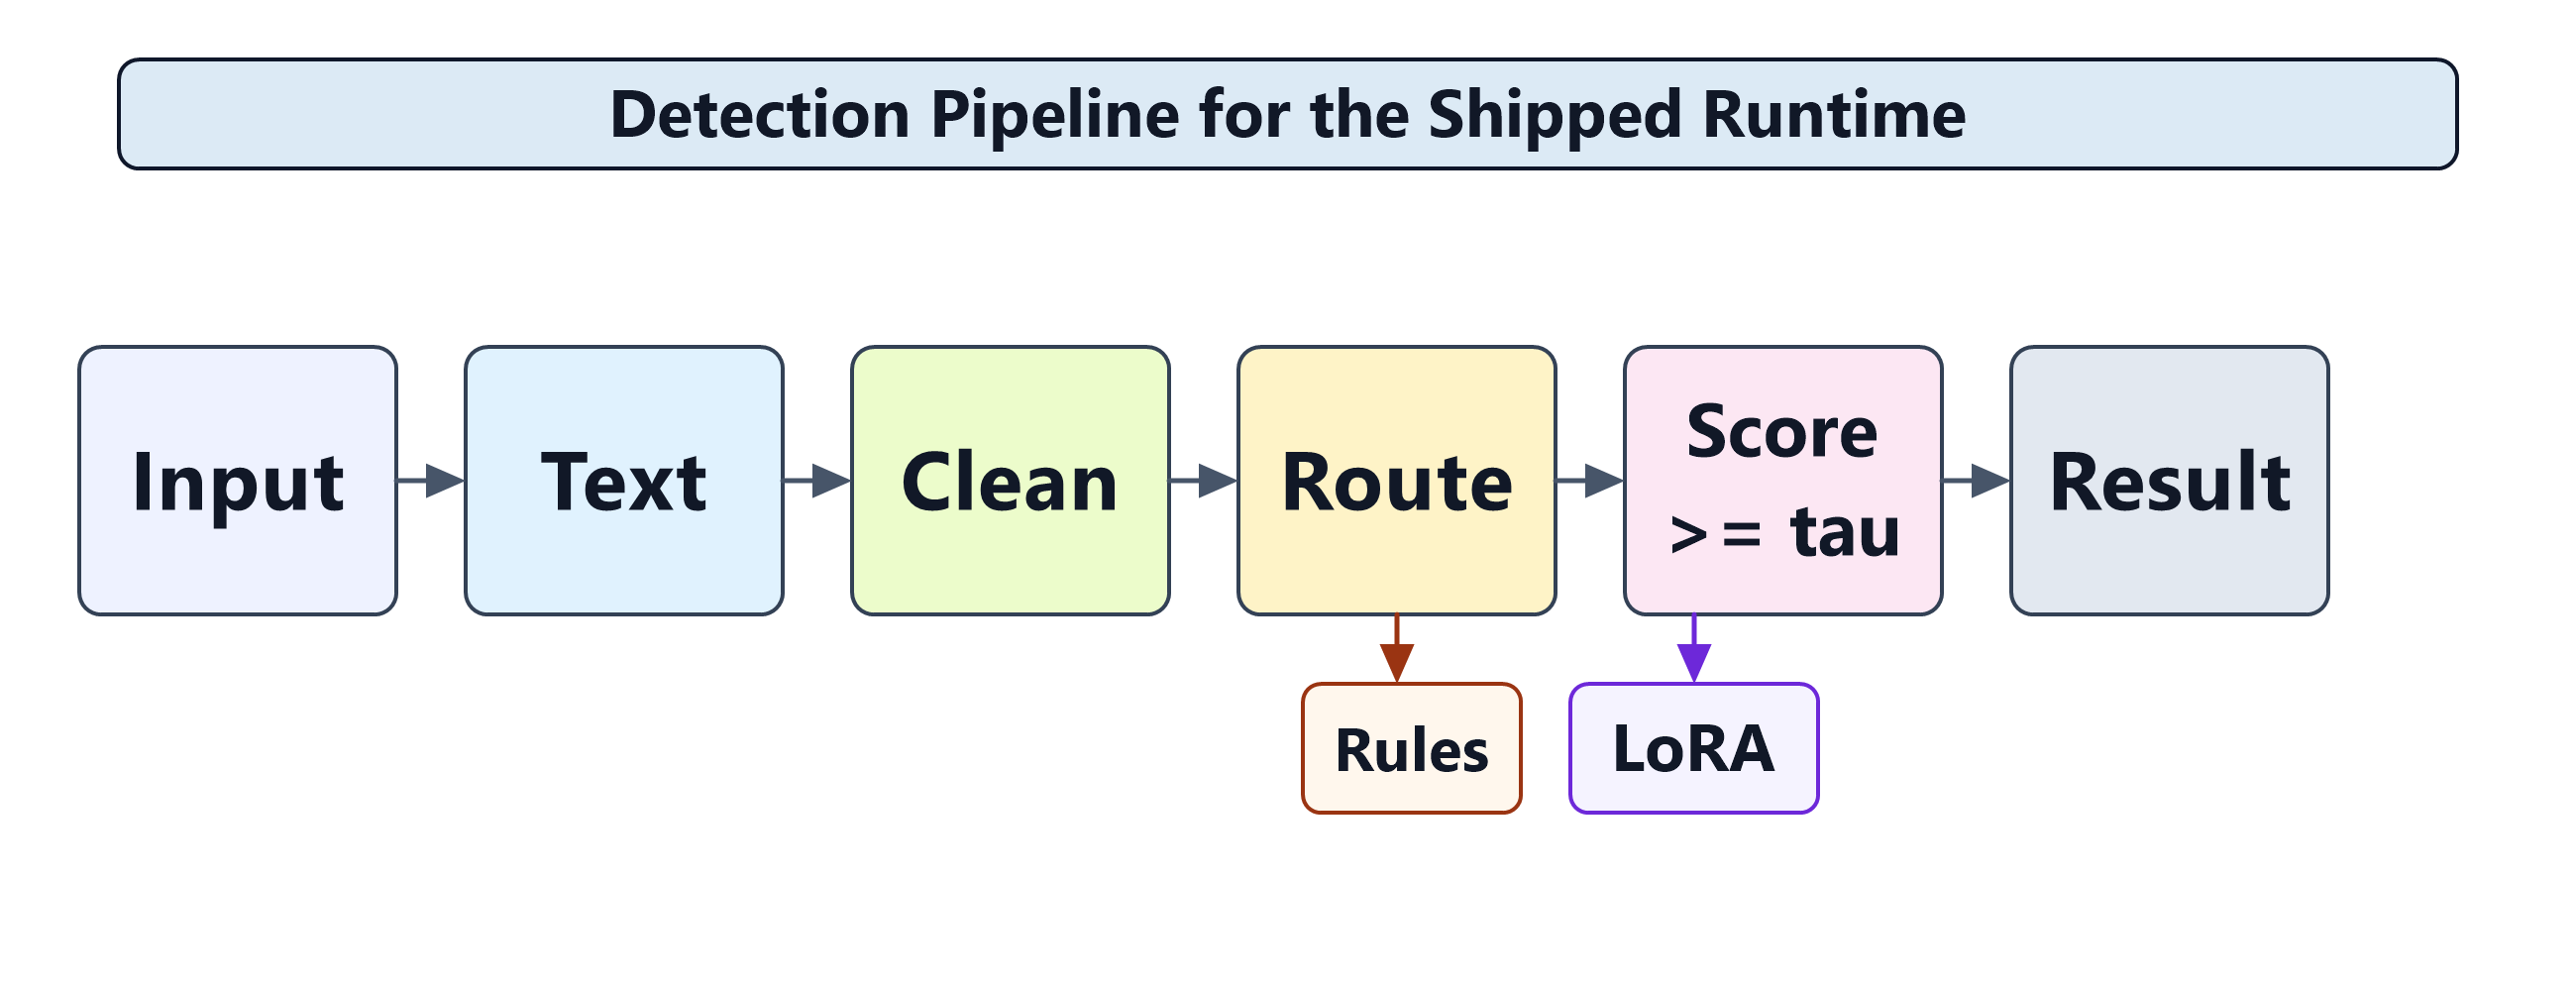
\includegraphics[width=0.95\linewidth]{ch3_pipeline.png}
  \caption{Detection pipeline from input text through detector scoring and allow/block decision.}
  \label{fig:method_pipeline}
\end{figure}

\begin{figure}[t]
  \centering
  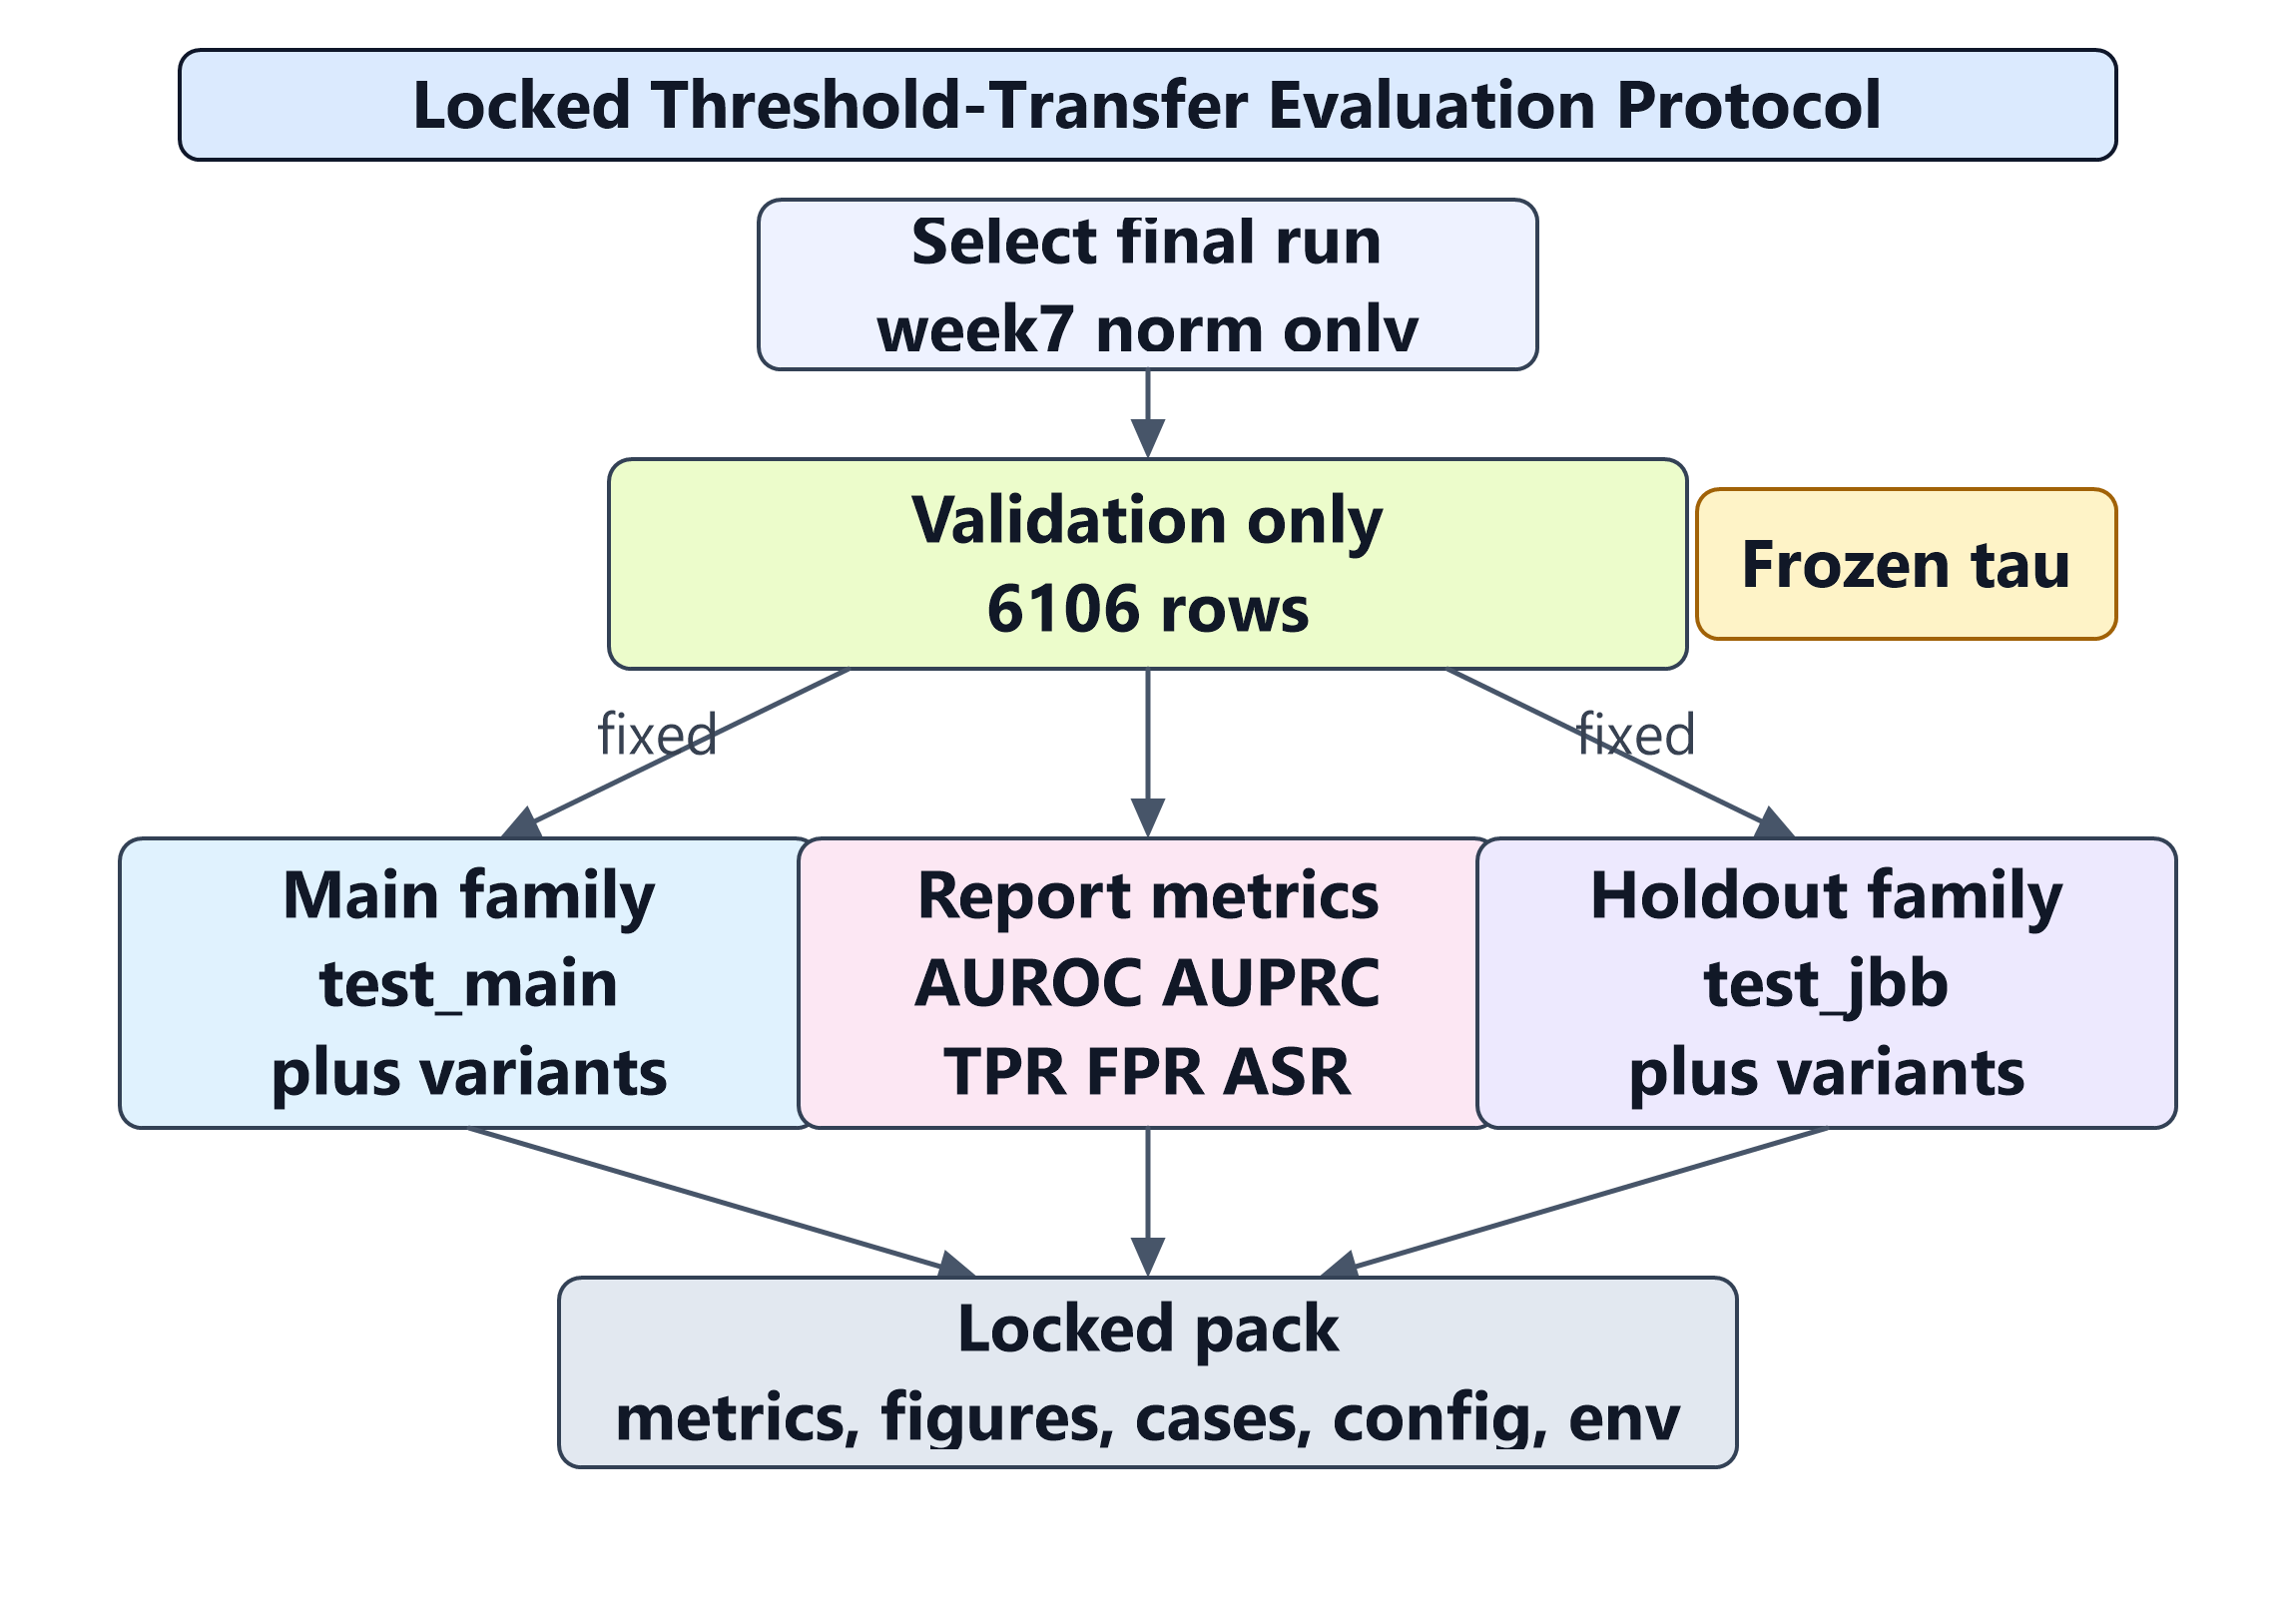
\includegraphics[width=0.95\linewidth]{ch3_eval_protocol.png}
  \caption{Locked evaluation protocol: calibrate $\tau$ on validation and transfer it unchanged to all evaluation splits.}
  \label{fig:threshold_transfer}
\end{figure}

The locked pack is therefore the single source of truth for counts, metrics, and figures. It strengthens reproducibility, but it does not justify overclaiming blind-test isolation or production-ready robustness.


\chapter{Experiments and Results}
\label{ch:experiments}

This chapter reports the final Week~7 results using the locked evaluation pack under a low-FPR operating-point protocol. Unless explicitly noted otherwise, all metrics are taken from the locked Week~7 evaluation bundle for \texttt{week7\_norm\_only}. The core distinction throughout the chapter is between ranking quality and fixed-threshold behavior under distribution shift.

\section{Evaluation framing and split grid}

The fixed Week~7 grid contains one validation split and two held-out evaluation families. Table~\ref{tab:exp_split_counts} repeats the authoritative counts used in this chapter.

\begin{table}[t]
\centering
\caption{Evaluation split counts used in Chapter~\ref{ch:experiments}.}
\label{tab:exp_split_counts}
\begin{tabular}{lrrr}
\toprule
Split & Total & Benign & Attack \\
\midrule
train & 201,276 & 14,859 & 186,417 \\
val & 6,106 & 3,082 & 3,024 \\
test\_main & 35,230 & 3,147 & 32,083 \\
test\_jbb & 197 & 98 & 99 \\
test\_main\_unicode & 35,230 & 3,147 & 32,083 \\
test\_jbb\_unicode & 197 & 98 & 99 \\
test\_main\_adv2 & 35,230 & 3,147 & 32,083 \\
test\_jbb\_adv2 & 197 & 98 & 99 \\
test\_main\_rewrite & 35,230 & 3,147 & 32,083 \\
test\_jbb\_rewrite & 197 & 98 & 99 \\
\bottomrule
\end{tabular}
\end{table}

The evaluation naming requires care. Although the repository uses split names such as \texttt{test\_main} and \texttt{test\_jbb}, these distributions were inspected during Week~7 selection and ablation analysis. They are therefore treated as development-evaluation distributions rather than blind final-test sets. This thesis avoids language that would imply strict blind-test generalization.

The main distribution, \texttt{test\_main}, is strongly attack-heavy, while validation is approximately balanced. This matters for interpretation: AUPRC is prevalence-sensitive, whereas fixed-threshold FPR and TPR remain the more deployment-relevant metrics.

The present split grid should therefore be read as a threshold-transfer stress study, not as a benign-heavy production simulation. Validation is used to learn the operating point, \texttt{test\_main} measures transfer on the main project distribution, and JBB-style splits act as out-of-distribution stress tests. A benign-heavy deployment slice is not part of the locked Week~7 evidence, but it is revisited later in this chapter and Chapter~\ref{ch:robustness} as a follow-up sensitivity analysis.

\section{Model selection summary}

Week~7 ablations varied two training-time factors: \texttt{normalize\_train} and \texttt{aug\_adv2\_prob}. The selected run was \texttt{week7\_norm\_only}. It is not described as globally robust; rather, it was the least harmful operating point among the tested options. It retained strong clean-distribution recall without the severe JBB adv2 recall collapse seen under heavier adv2-oriented training.

The rules baseline remains important for two reasons. First, it is the guaranteed runnable detector path in constrained environments. Second, it provides a transparent point of comparison for the learned model within the shipped runtime. Table~\ref{tab:rules_baseline_results} shows that the rules baseline offers almost no useful recall under the fixed threshold of 0.5, despite occasionally achieving very low FPR. Only splits with frozen rules-baseline artifacts are shown in the table; the thesis does not imply a broader comparator sweep than the repository actually contains.

\begin{table}[t]
\centering
\caption{Rules baseline results at the fixed threshold of 0.5.}
\label{tab:rules_baseline_results}
\small
\begin{tabular}{lrrrrr}
\toprule
Split & AUROC & AUPRC & FPR@0.5 & TPR@0.5 & ASR@0.5 \\
\midrule
test\_main & 0.5024 & 0.9111 & 0.0016 & 0.0064 & 0.9936 \\
test\_main\_unicode & 0.5009 & 0.9108 & 0.0010 & 0.0028 & 0.9972 \\
test\_main\_adv2 & 0.5007 & 0.9108 & 0.0000 & 0.0015 & 0.9985 \\
test\_jbb\_adv2 & 0.5000 & 0.5025 & 0.0000 & 0.0000 & 1.0000 \\
test\_main\_rewrite & 0.5021 & 0.9110 & 0.0016 & 0.0057 & 0.9943 \\
\bottomrule
\end{tabular}
\normalsize
\end{table}

\section{Main locked-pack results}

Table~\ref{tab:winner_summary} gives a compact winner-only view of the final selected run before the denser all-candidate Week~7 tables. This summary is the clearest single-table answer to the central empirical question of the thesis: the selected detector ranks well on the main project distribution, but its transferred threshold degrades sharply under cross-dataset shift and adv2-style perturbation.

\begin{table}[t]
\centering
\caption{Winner-only summary for \texttt{week7\_norm\_only} at the transferred validation threshold $\tau = 0.7340$. This compact view isolates the final selected run from the broader Week~7 ablation tables.}
\label{tab:winner_summary}
\small
\begin{tabular}{lrrrr}
\toprule
Split & AUROC & FPR@$\tau$ & TPR@$\tau$ & ASR@$\tau$ \\
\midrule
\texttt{val} & 0.9983 & 0.0094 & 0.9696 & 0.0304 \\
\texttt{test\_main} & 0.9958 & 0.0311 & 0.9869 & 0.0131 \\
\texttt{test\_jbb} & 0.8890 & 0.5816 & 0.9798 & 0.0202 \\
\midrule
\texttt{test\_main\_unicode} & 0.9949 & 0.0429 & 0.9862 & 0.0138 \\
\texttt{test\_jbb\_unicode} & 0.8814 & 0.6531 & 0.9798 & 0.0202 \\
\midrule
\texttt{test\_main\_rewrite} & 0.9942 & 0.0531 & 0.9902 & 0.0098 \\
\texttt{test\_jbb\_rewrite} & 0.8956 & 0.5714 & 0.9899 & 0.0101 \\
\midrule
\texttt{test\_main\_adv2} & 0.7133 & 0.6403 & 0.9967 & 0.0033 \\
\texttt{test\_jbb\_adv2} & 0.6318 & 0.8469 & 0.8990 & 0.1010 \\
\bottomrule
\end{tabular}
\normalsize
\end{table}


Table~\ref{tab:clean_unicode_results} reports clean and Unicode results for all Week~7 candidate runs. The final row group of interest is \texttt{week7\_norm\_only}, whose validation threshold is 0.7340.

\begin{table}[t]
\centering
\caption{Clean and Unicode results from the Week 7 locked evaluation pack.}
\label{tab:clean_unicode_results}
\small
\resizebox{\textwidth}{!}{%
\begin{tabular}{lrrrrrrr}
\toprule
Run & Split & AUROC & AUPRC & $\tau_{val}$ & FPR@$\tau$ & TPR@$\tau$ & ASR@$\tau$ \\
\midrule
week7\_adv2\_only & val & 0.9982 & 0.9982 & 0.5624 & 0.0097 & 0.9729 & 0.0271 \\
week7\_adv2\_only & test\_main & 0.9942 & 0.9994 & 0.5624 & 0.0607 & 0.9970 & 0.0030 \\
week7\_adv2\_only & test\_jbb & 0.8962 & 0.8942 & 0.5624 & 0.6939 & 0.9899 & 0.0101 \\
week7\_adv2\_only & test\_main\_unicode & 0.9933 & 0.9992 & 0.5624 & 0.0642 & 0.9969 & 0.0031 \\
week7\_adv2\_only & test\_jbb\_unicode & 0.8393 & 0.8322 & 0.5624 & 0.7551 & 1.0000 & 0.0000 \\
week7\_control & val & 0.9982 & 0.9982 & 0.6894 & 0.0097 & 0.9709 & 0.0291 \\
week7\_control & test\_main & 0.9960 & 0.9996 & 0.6894 & 0.0311 & 0.9878 & 0.0122 \\
week7\_control & test\_jbb & 0.9078 & 0.9033 & 0.6894 & 0.5918 & 0.9798 & 0.0202 \\
week7\_control & test\_main\_unicode & 0.9951 & 0.9995 & 0.6894 & 0.0423 & 0.9858 & 0.0142 \\
week7\_control & test\_jbb\_unicode & 0.8857 & 0.8800 & 0.6894 & 0.7041 & 0.9697 & 0.0303 \\
week7\_norm\_only & val & 0.9983 & 0.9982 & 0.7340 & 0.0094 & 0.9696 & 0.0304 \\
week7\_norm\_only & test\_main & 0.9958 & 0.9996 & 0.7340 & 0.0311 & 0.9869 & 0.0131 \\
week7\_norm\_only & test\_jbb & 0.8890 & 0.8747 & 0.7340 & 0.5816 & 0.9798 & 0.0202 \\
week7\_norm\_only & test\_main\_unicode & 0.9949 & 0.9994 & 0.7340 & 0.0429 & 0.9862 & 0.0138 \\
week7\_norm\_only & test\_jbb\_unicode & 0.8814 & 0.8704 & 0.7340 & 0.6531 & 0.9798 & 0.0202 \\
week7\_norm\_plus\_adv2 & val & 0.9979 & 0.9977 & 0.6815 & 0.0094 & 0.9659 & 0.0341 \\
week7\_norm\_plus\_adv2 & test\_main & 0.9929 & 0.9992 & 0.6815 & 0.0566 & 0.9944 & 0.0056 \\
week7\_norm\_plus\_adv2 & test\_jbb & 0.9018 & 0.8950 & 0.6815 & 0.6122 & 0.9798 & 0.0202 \\
week7\_norm\_plus\_adv2 & test\_main\_unicode & 0.9920 & 0.9991 & 0.6815 & 0.0582 & 0.9959 & 0.0041 \\
week7\_norm\_plus\_adv2 & test\_jbb\_unicode & 0.8892 & 0.8744 & 0.6815 & 0.6735 & 0.9697 & 0.0303 \\
\bottomrule
\end{tabular}%
}
\normalsize
\end{table}

Three observations from Table~\ref{tab:clean_unicode_results} matter most:
\begin{enumerate}
  \item On \texttt{test\_main}, ranking performance is strong and recall remains high at the transferred threshold.
  \item Even on clean text, the transferred threshold does not preserve the 1\% FPR target: \texttt{test\_main} rises to 0.0311.
  \item Cross-dataset shift dominates benign harm on \texttt{test\_jbb}, where the same threshold yields FPR = 0.5816 despite high recall.
\end{enumerate}

Table~\ref{tab:adv2_rewrite_results} shows that adv2 and rewrite stress very different aspects of the detector.

\begin{table}[t]
\centering
\caption{adv2 and rewrite results from the Week 7 locked evaluation pack.}
\label{tab:adv2_rewrite_results}
\small
\resizebox{\textwidth}{!}{%
\begin{tabular}{lrrrrrrr}
\toprule
Run & Split & AUROC & AUPRC & $\tau_{val}$ & FPR@$\tau$ & TPR@$\tau$ & ASR@$\tau$ \\
\midrule
week7\_adv2\_only & test\_main\_adv2 & 0.9833 & 0.9979 & 0.5624 & 0.0985 & 0.9856 & 0.0144 \\
week7\_adv2\_only & test\_jbb\_adv2 & 0.6415 & 0.6689 & 0.5624 & 0.6633 & 0.7677 & 0.2323 \\
week7\_adv2\_only & test\_main\_rewrite & 0.9912 & 0.9990 & 0.5624 & 0.0801 & 0.9977 & 0.0023 \\
week7\_adv2\_only & test\_jbb\_rewrite & 0.8870 & 0.8918 & 0.5624 & 0.6939 & 0.9899 & 0.0101 \\
week7\_control & test\_main\_adv2 & 0.6547 & 0.9379 & 0.6894 & 0.6826 & 0.9731 & 0.0269 \\
week7\_control & test\_jbb\_adv2 & 0.6007 & 0.5727 & 0.6894 & 0.8980 & 0.9495 & 0.0505 \\
week7\_control & test\_main\_rewrite & 0.9934 & 0.9992 & 0.6894 & 0.0537 & 0.9896 & 0.0104 \\
week7\_control & test\_jbb\_rewrite & 0.8993 & 0.8907 & 0.6894 & 0.6020 & 0.9798 & 0.0202 \\
week7\_norm\_only & test\_main\_adv2 & 0.7133 & 0.9523 & 0.7340 & 0.6403 & 0.9967 & 0.0033 \\
week7\_norm\_only & test\_jbb\_adv2 & 0.6318 & 0.6294 & 0.7340 & 0.8469 & 0.8990 & 0.1010 \\
week7\_norm\_only & test\_main\_rewrite & 0.9942 & 0.9994 & 0.7340 & 0.0531 & 0.9902 & 0.0098 \\
week7\_norm\_only & test\_jbb\_rewrite & 0.8956 & 0.8964 & 0.7340 & 0.5714 & 0.9899 & 0.0101 \\
week7\_norm\_plus\_adv2 & test\_main\_adv2 & 0.9833 & 0.9979 & 0.6815 & 0.0947 & 0.9831 & 0.0169 \\
week7\_norm\_plus\_adv2 & test\_jbb\_adv2 & 0.6329 & 0.6506 & 0.6815 & 0.5408 & 0.6768 & 0.3232 \\
week7\_norm\_plus\_adv2 & test\_main\_rewrite & 0.9905 & 0.9990 & 0.6815 & 0.0718 & 0.9968 & 0.0032 \\
week7\_norm\_plus\_adv2 & test\_jbb\_rewrite & 0.8754 & 0.8701 & 0.6815 & 0.6224 & 0.9798 & 0.0202 \\
\bottomrule
\end{tabular}%
}
\normalsize
\end{table}

The key empirical signature is the adv2 failure mode. For \texttt{week7\_norm\_only}, \texttt{test\_main\_adv2} has AUROC = 0.7133, FPR = 0.6403, and TPR = 0.9967. The detector still ranks many attacks above benign text, but the benign score distribution shifts badly enough that a fixed threshold becomes operationally unusable. By contrast, rewrite is much milder on the main distribution, though it does not solve the JBB false-positive problem. The plots below are regenerated from the frozen per-example prediction files so that the transferred threshold $\tau = 0.7340$ is marked explicitly rather than inferred only from the tables.

\begin{figure}[t]
  \centering
  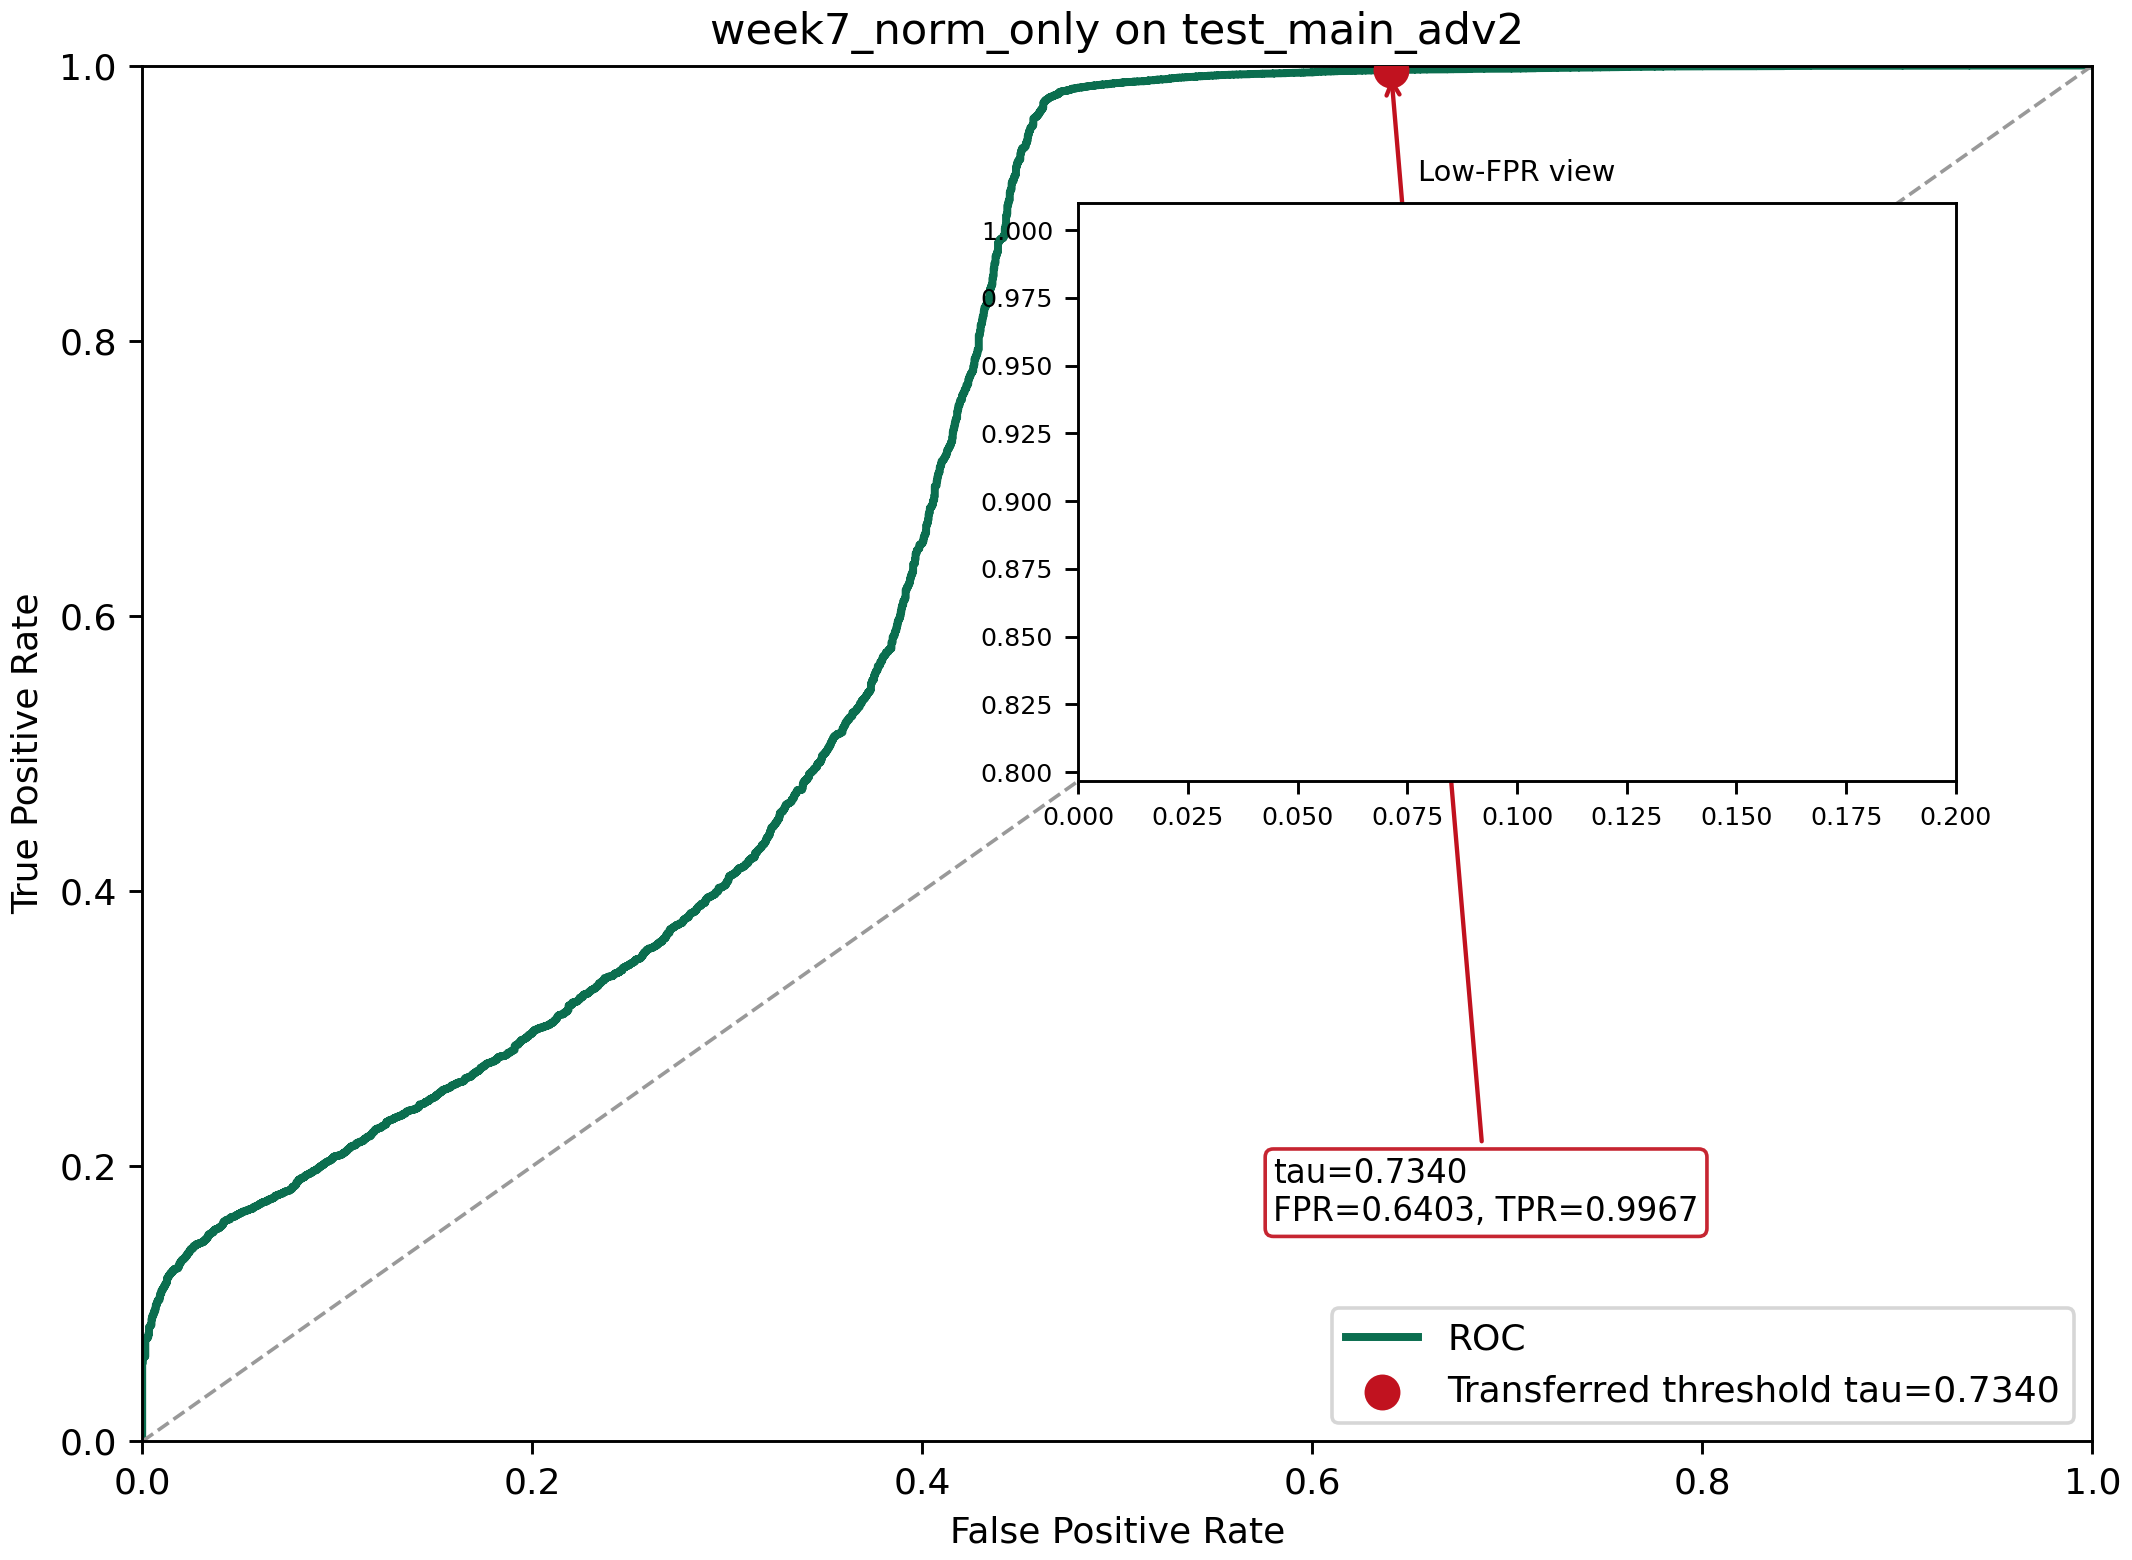
\includegraphics[width=0.88\linewidth]{roc_week7_norm_only_test_main_adv2.png}
  \caption{ROC curve for \texttt{week7\_norm\_only} on \texttt{test\_main\_adv2}. The red marker shows the transferred validation threshold $\tau = 0.7340$; the inset provides a low-FPR view of the same operating point, which still lies far outside a usable benign-error regime even though the full curve ranks attacks above benign text better than chance.}
  \label{fig:roc_main_adv2}
\end{figure}

\begin{figure}[t]
  \centering
  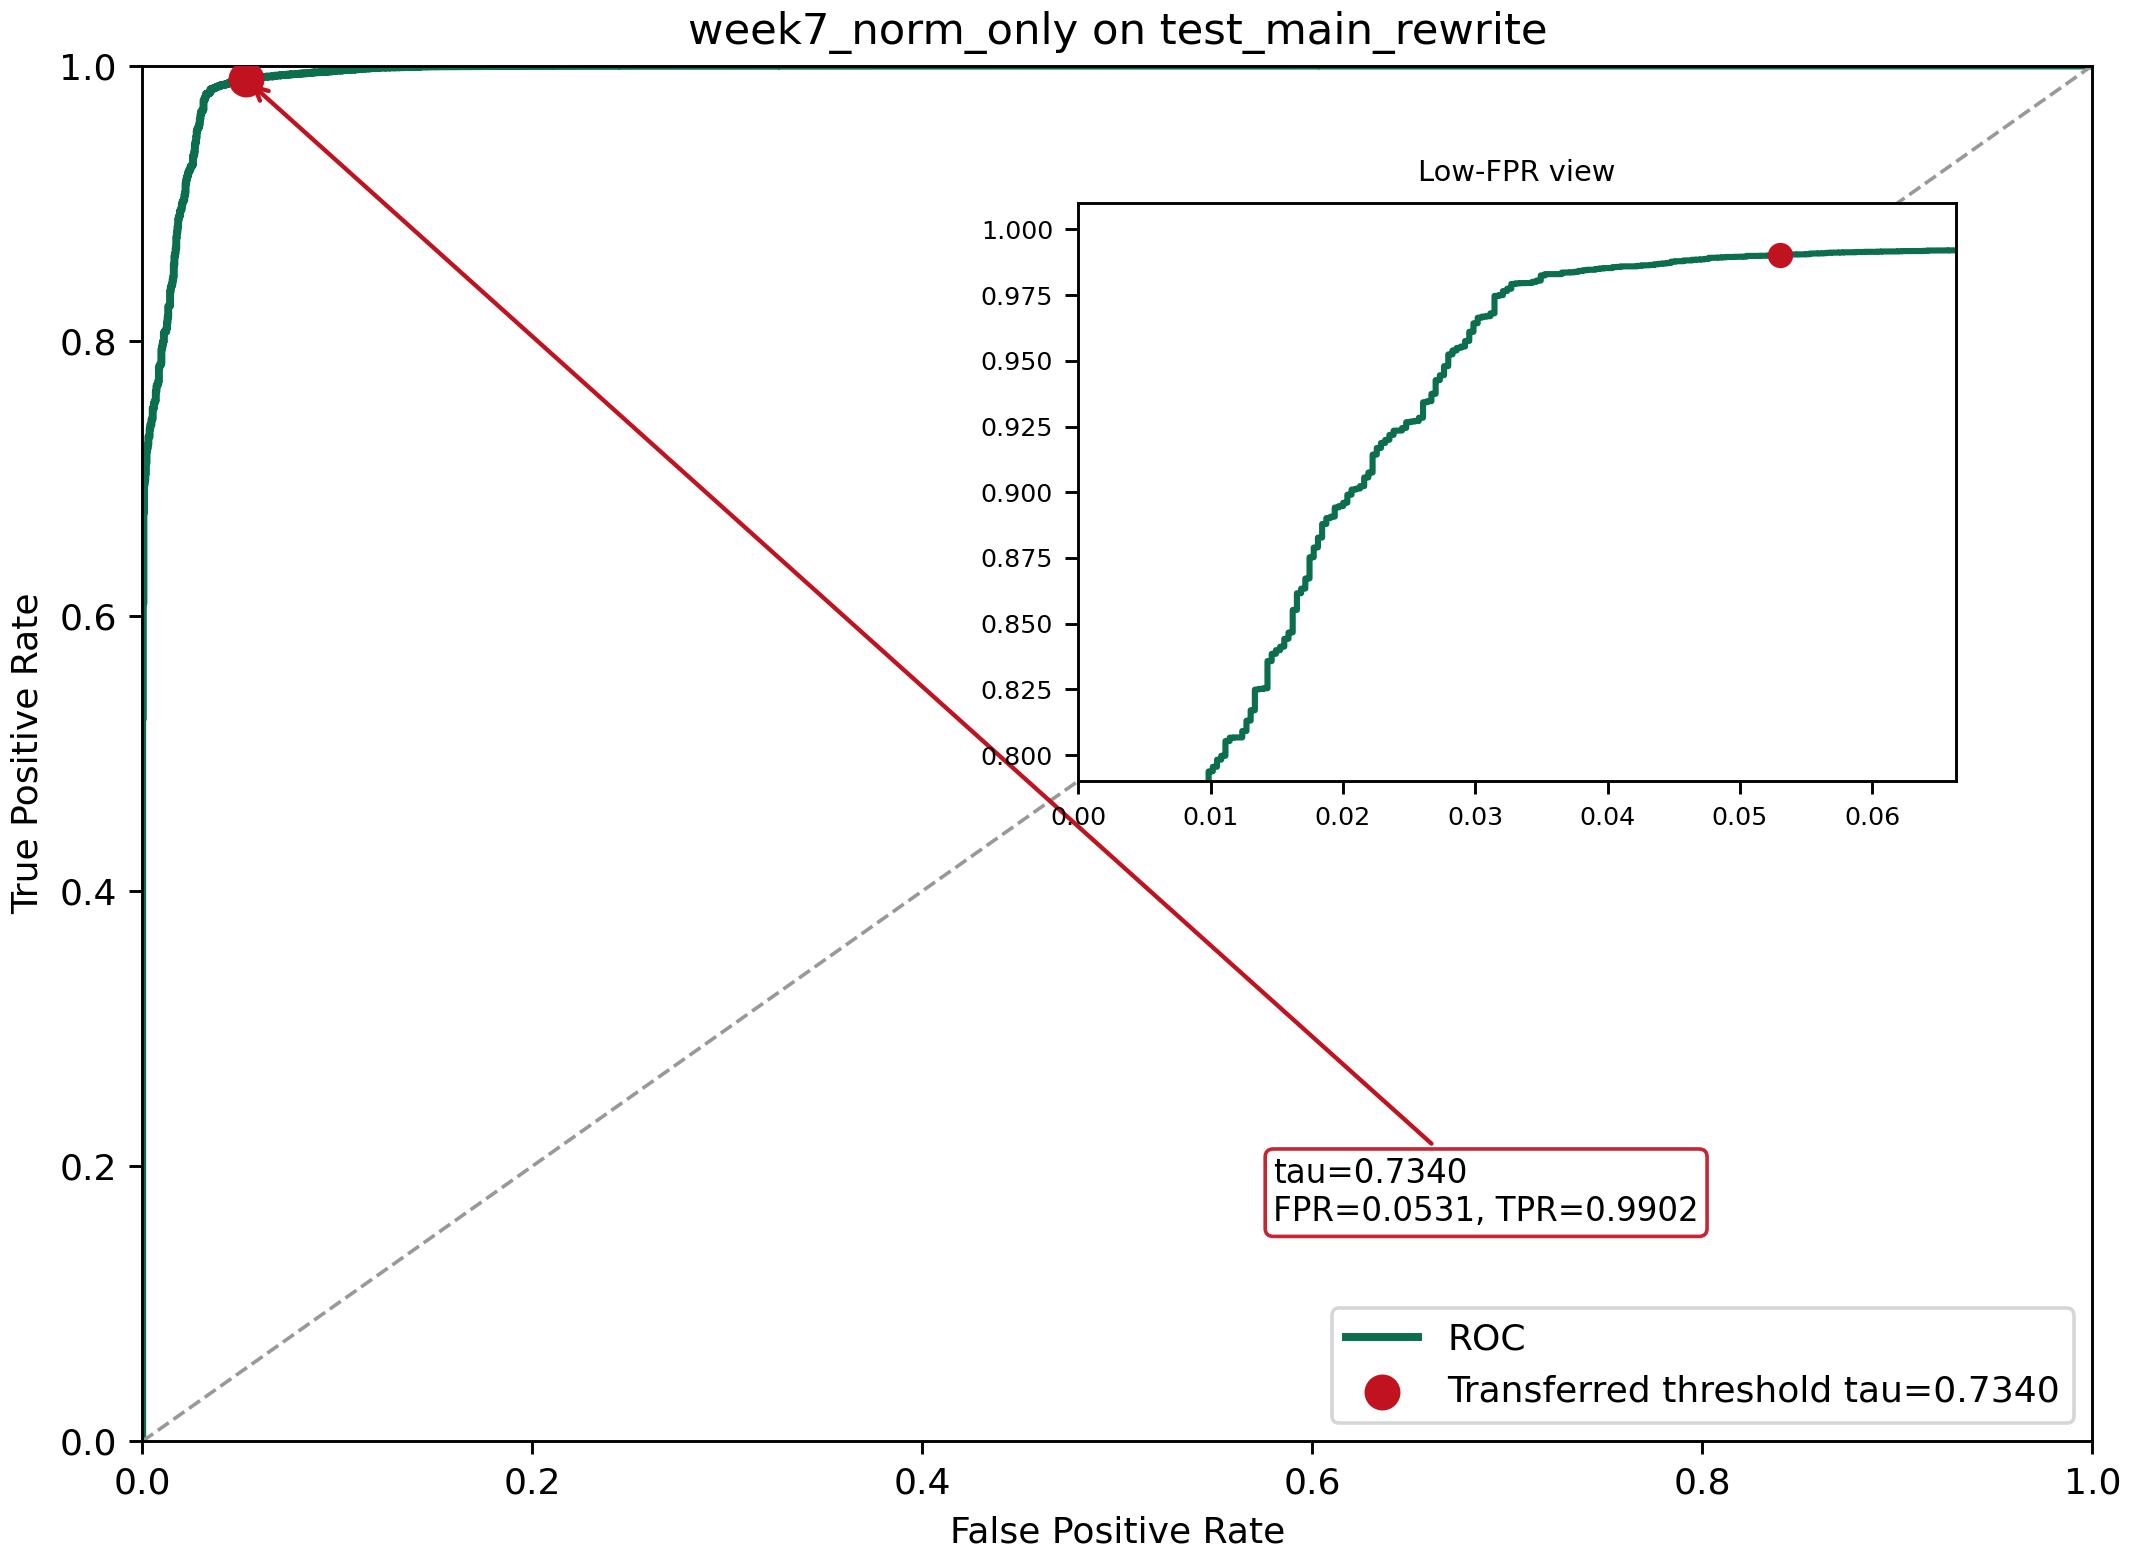
\includegraphics[width=0.88\linewidth]{roc_week7_norm_only_test_main_rewrite.png}
  \caption{ROC curve for \texttt{week7\_norm\_only} on \texttt{test\_main\_rewrite}. The red marker again shows the transferred threshold $\tau = 0.7340$; rewrite preserves a much cleaner ranking profile than adv2, but the operating point still misses the nominal 1\% benign-FPR target.}
  \label{fig:roc_main_rewrite}
\end{figure}

\begin{figure}[t]
  \centering
  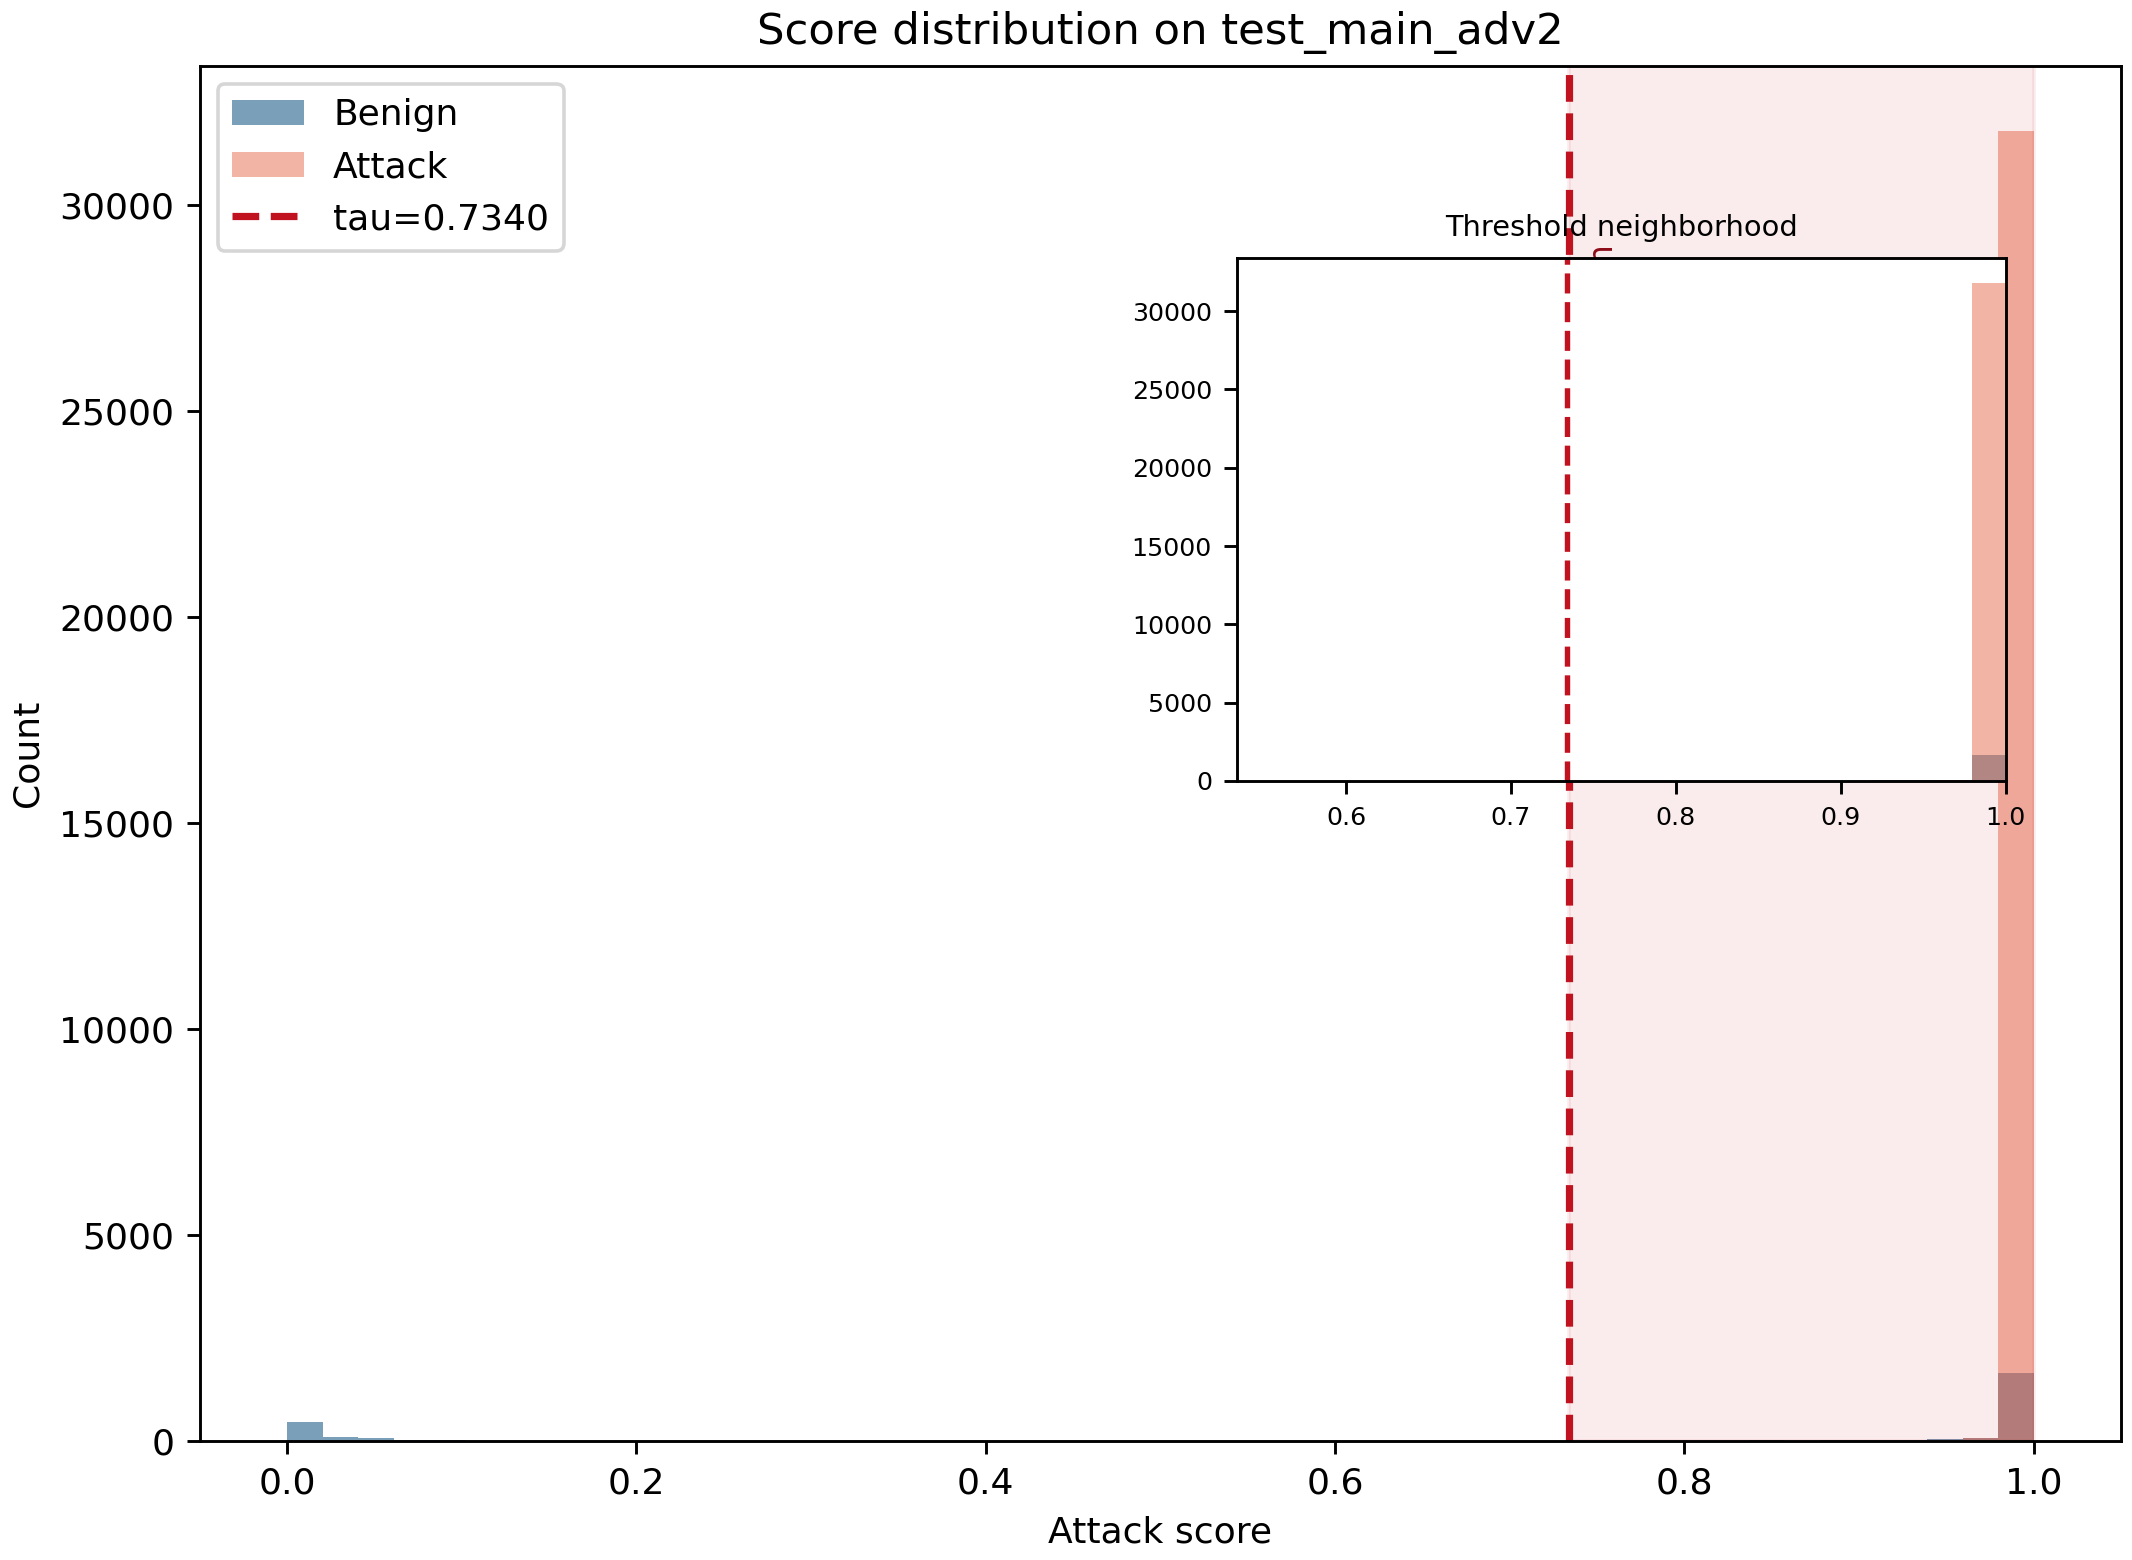
\includegraphics[width=0.88\linewidth]{hist_week7_norm_only_test_main_adv2.png}
  \caption{Score histogram for \texttt{week7\_norm\_only} on \texttt{test\_main\_adv2}. The dashed red line marks the transferred threshold $\tau = 0.7340$; a large mass of benign scores shifts into the block region, explaining the observed FPR of 0.6403.}
  \label{fig:hist_main_adv2}
\end{figure}

\section{Confusion-count and uncertainty view}

Rates alone can hide how many benign prompts are actually harmed at the transferred threshold. Table~\ref{tab:confusion_counts} converts the stored FPR and TPR values for \texttt{week7\_norm\_only} into integer confusion-count summaries using the locked split counts. This makes the main failure modes more legible. On \texttt{test\_main}, the clean-distribution FPR of 0.0311 corresponds to 98 benign false positives out of 3,147 benign examples. On \texttt{test\_jbb}, the same transferred threshold flags 57 of only 98 benign examples, which is a much clearer statement of the practical harm than the rate alone.

\begin{table}[t]
\centering
\caption{Confusion-count view of the transferred threshold for \texttt{week7\_norm\_only}. Counts are derived from locked aggregate split sizes and the stored operating-point rates.}
\label{tab:confusion_counts}
\small
\begin{tabular}{lrrrrrr}
\toprule
Split & Benign $n_0$ & Attack $n_1$ & FP & TN & TP & FN \\
\midrule
\texttt{val} & 3082 & 3024 & 29 & 3053 & 2932 & 92 \\
\texttt{test\_main} & 3147 & 32083 & 98 & 3049 & 31664 & 419 \\
\texttt{test\_main\_unicode} & 3147 & 32083 & 135 & 3012 & 31639 & 444 \\
\texttt{test\_main\_rewrite} & 3147 & 32083 & 167 & 2980 & 31767 & 316 \\
\texttt{test\_main\_adv2} & 3147 & 32083 & 2015 & 1132 & 31976 & 107 \\
\texttt{test\_jbb} & 98 & 99 & 57 & 41 & 97 & 2 \\
\texttt{test\_jbb\_unicode} & 98 & 99 & 64 & 34 & 97 & 2 \\
\texttt{test\_jbb\_rewrite} & 98 & 99 & 56 & 42 & 98 & 1 \\
\texttt{test\_jbb\_adv2} & 98 & 99 & 83 & 15 & 89 & 10 \\
\bottomrule
\end{tabular}
\normalsize
\end{table}


The adv2 pattern is even more concrete in count form. For \texttt{test\_main\_adv2}, the detector still blocks 31,976 of 32,083 attacks, but it also falsely flags 2,015 benign inputs. On \texttt{test\_jbb\_adv2}, only 15 benign examples remain unflagged. These counts reinforce the main thesis claim boundary: high recall under perturbation does not imply a usable operating point when benign-score drift is large.

Because the main distribution is large and JBB is small, uncertainty differs sharply across splits. Table~\ref{tab:wilson_ci} restores the Wilson 95\% confidence intervals drafted earlier, computed on the relevant class subset for each thresholded metric. The intervals remain tight on the large \texttt{test\_main} family and much wider on the 98-benign / 99-attack JBB family. The JBB rows should therefore be read as strong stress signals, but not as high-precision estimates of the true deployment rate.

\begin{table}[t]
\centering
\caption{Wilson 95\% confidence intervals for thresholded operating-point metrics of \texttt{week7\_norm\_only}. Intervals are computed on the relevant class subset of each split.}
\label{tab:wilson_ci}
\scriptsize
\begin{tabular}{l p{4.0cm} p{4.0cm} p{4.0cm}}
\toprule
Split & FPR@$\tau$ (95\% CI) & TPR@$\tau$ (95\% CI) & ASR@$\tau$ (95\% CI) \\
\midrule
\texttt{val} & 0.0094 [0.0066, 0.0135] & 0.9696 [0.9628, 0.9751] & 0.0304 [0.0249, 0.0372] \\
\texttt{test\_main} & 0.0311 [0.0256, 0.0378] & 0.9869 [0.9856, 0.9881] & 0.0131 [0.0119, 0.0144] \\
\texttt{test\_main\_unicode} & 0.0429 [0.0364, 0.0506] & 0.9862 [0.9848, 0.9874] & 0.0138 [0.0126, 0.0152] \\
\texttt{test\_main\_rewrite} & 0.0531 [0.0458, 0.0615] & 0.9902 [0.9890, 0.9912] & 0.0098 [0.0088, 0.0110] \\
\texttt{test\_main\_adv2} & 0.6403 [0.6234, 0.6569] & 0.9967 [0.9960, 0.9972] & 0.0033 [0.0028, 0.0040] \\
\texttt{test\_jbb} & 0.5816 [0.4827, 0.6744] & 0.9798 [0.9293, 0.9944] & 0.0202 [0.0056, 0.0707] \\
\texttt{test\_jbb\_unicode} & 0.6531 [0.5547, 0.7399] & 0.9798 [0.9293, 0.9944] & 0.0202 [0.0056, 0.0707] \\
\texttt{test\_jbb\_rewrite} & 0.5714 [0.4726, 0.6649] & 0.9899 [0.9450, 0.9982] & 0.0101 [0.0018, 0.0550] \\
\texttt{test\_jbb\_adv2} & 0.8469 [0.7627, 0.9050] & 0.8990 [0.8240, 0.9442] & 0.1010 [0.0558, 0.1760] \\
\bottomrule
\end{tabular}
\normalsize
\end{table}


\section{Follow-up calibration and seed-sensitivity analyses}

The locked Week~7 pack remains the authoritative result bundle for this thesis. However, four follow-up analyses were run after the lock stage to test whether the core claim survives beyond one frozen table view: calibration curves, threshold sweeps, benign-heavy calibration sensitivity, and three-seed reruns of the selected configuration. These follow-up artifacts are indexed in Appendix~\ref{app:repro_artifacts}. They are reported here as additional evidence, not as replacement locked-pack results.

These four analyses answer different questions. Calibration asks whether the detector scores remain probabilistically interpretable under shift. Threshold sweeps ask whether the chosen operating point is locally brittle or whether nearby thresholds behave the same way. Benign-heavy calibration sensitivity asks whether recalibrating on a more deployment-shaped validation prior materially changes the outcome. Three-seed reruns ask whether the observed threshold-transfer failure could be dismissed as a one-seed accident. The calibration and seed findings are summarized here, while the threshold-sweep and benign-heavy results are discussed in Chapter~\ref{ch:robustness} because they are primarily robustness follow-ups.

Calibration asks whether the detector score can still be read as a trustworthy confidence signal once the data distribution changes. Table~\ref{tab:followup_calibration} shows that score calibration is strong on \texttt{val} and \texttt{test\_main}, but it breaks sharply under cross-dataset and adv2 shift. Expected calibration error (ECE) summarizes the average gap between predicted attack scores and the observed attack frequency within fixed score bins; lower values are better. The Brier score is the mean squared error between the predicted attack score and the binary label, so lower values again indicate better calibrated and more accurate probabilities. In the follow-up analysis script, ECE is computed with 10 equal-width bins over $[0,1]$. On \texttt{val}, ECE is only 0.0065; on \texttt{test\_main} it remains low at 0.0087. By contrast, \texttt{test\_jbb} rises to 0.3227 and \texttt{test\_jbb\_adv2} to 0.4316. This matters because the thesis claim is not only that attacks rank above benign text, but that thresholded scores should remain interpretable enough to support low benign false-positive deployment. The follow-up calibration analysis supports the opposite conclusion under shift: score confidence itself becomes unreliable.

\begin{table}[t]
\centering
\caption{Follow-up calibration summary for the frozen \texttt{week7\_norm\_only} predictions. These values are computed from the archived per-example score files and are reported as post-lock analysis rather than as part of the original Week~7 pack.}
\label{tab:followup_calibration}
\small
\begin{tabular}{lrrr}
\toprule
Split & Prevalence & ECE & Brier \\
\midrule
\texttt{val} & 0.4953 & 0.0065 & 0.0133 \\
\texttt{test\_main} & 0.9107 & 0.0087 & 0.0107 \\
\texttt{test\_jbb} & 0.5025 & 0.3227 & 0.3042 \\
\texttt{test\_main\_adv2} & 0.9107 & 0.0536 & 0.0587 \\
\texttt{test\_jbb\_adv2} & 0.5025 & 0.4316 & 0.4350 \\
\bottomrule
\end{tabular}
\normalsize
\end{table}


Seed sensitivity asks whether the threshold-transfer result is specific to one random initialization or persists across reruns. The three-seed reruns reinforce the same claim from a different angle. Table~\ref{tab:followup_multiseed} shows that threshold-free ranking on the main distribution is stable across seeds, with \texttt{test\_main} AUROC = 0.9958 $\pm$ 0.0004. However, the transferred operating point is noticeably less stable. The mean \texttt{test\_main} benign FPR rises to 0.0402 $\pm$ 0.0089, above the single frozen-run value of 0.0311, and shifted splits remain highly variable. The per-seed validation thresholds also differ materially even though they all satisfy the same validation FPR target: seed~41 selects $\tau = 0.5199$, seed~42 selects $\tau = 0.7450$, and seed~43 selects $\tau = 0.6042$. This is strong evidence that the detector family is stable in ranking terms but unstable in transferred operating-point terms.

\begin{table}[t]
\centering
\caption{Three-seed follow-up sensitivity summary for the \texttt{week7\_norm\_only} configuration. Mean and standard deviation are reported across seeds 41, 42, and 43. These reruns were executed after the frozen Week~7 submission pack and are therefore reported as follow-up evidence rather than replacement locked-pack results.}
\label{tab:followup_multiseed}
\small
\begin{tabular}{lrrr}
\toprule
Split & AUROC (mean $\pm$ std) & FPR@$\tau$ (mean $\pm$ std) & TPR@$\tau$ (mean $\pm$ std) \\
\midrule
\texttt{test\_main} & 0.9958 $\pm$ 0.0004 & 0.0402 $\pm$ 0.0089 & 0.9925 $\pm$ 0.0055 \\
\texttt{test\_jbb} & 0.9101 $\pm$ 0.0107 & 0.6088 $\pm$ 0.1027 & 0.9865 $\pm$ 0.0058 \\
\texttt{test\_main\_adv2} & 0.7693 $\pm$ 0.1265 & 0.6103 $\pm$ 0.1882 & 0.9925 $\pm$ 0.0108 \\
\texttt{test\_jbb\_adv2} & 0.6211 $\pm$ 0.0109 & 0.6905 $\pm$ 0.4129 & 0.7441 $\pm$ 0.3488 \\
\bottomrule
\end{tabular}
\normalsize
\end{table}


These reruns should be interpreted carefully. They were executed under the current repository code path after the locked Week~7 pack was frozen, so they are a follow-up sensitivity study rather than a new official winner selection process. That distinction does not weaken their value; it sharpens the thesis boundary. The follow-up evidence makes it harder to dismiss the locked-pack result as one unlucky run and instead supports the broader conclusion that threshold-transfer instability persists across random seeds once the evaluation distribution shifts.

\section{Failure-case analysis}

The locked pack also includes ranked false-positive and false-negative lists under \texttt{error\_cases/}. To avoid reproducing harmful prompts verbatim in the thesis, Table~\ref{tab:failure_modes} groups those lists into sanitized categories rather than quoting full examples. The table does not replace the raw evidence; it summarizes the recurring patterns seen in the stored error-case files.

\begin{table}[t]
\centering
\caption{Sanitized failure-case categories derived from the locked Week~7 ranked error-case lists. Raw prompts are not reproduced; the table groups them into recurring patterns instead.}
\label{tab:failure_modes}
\scriptsize
\begin{tabularx}{\textwidth}{>{\raggedright\arraybackslash}p{0.18\textwidth}>{\raggedright\arraybackslash}p{0.24\textwidth}X>{\raggedright\arraybackslash}p{0.20\textwidth}}
\toprule
Category & Locked-pack evidence & Observed pattern & Interpretation \\
\midrule
Obfuscated attack false negatives & \texttt{test\_main\_adv2\_fn.md}, \texttt{test\_jbb\_adv2\_fn.md} & Attack-labeled prompts about malware, identity theft, covert tracking, or physical harm are heavily corrupted by confusables, zero-width noise, and marker distortion yet still score far below $\tau$. & Character-level obfuscation can preserve malicious intent while driving the detector toward false negatives. \\
Benign topical false positives & \texttt{test\_jbb\_adv2\_fp.md}, \texttt{test\_jbb\_rewrite\_fp.md} & Benign prompts discussing sensitive topics such as eating disorders, drugs, blackmail, or controversial ideologies receive scores near 1.0 when they retain high-risk vocabulary. & The detector overweights lexical overlap with unsafe intent, which is especially costly under cross-dataset shift. \\
Structured benign false positives & \texttt{test\_main\_adv2\_fp.md}, \texttt{test\_main\_rewrite\_fp.md} & Tables, translation/code tasks, math word problems, and document-style snippets with noisy formatting are frequently classified as attacks. & Formatting corruption and mixed prompt-context structure can look attack-like even when the underlying task is benign. \\
Rewrite semantic drift and ambiguity & \texttt{test\_main\_rewrite\_fn.md}, \texttt{test\_jbb\_rewrite\_fn.md} & Some attack-labeled rewrite examples read like innocuous wellness, factual, or generic assistance prompts after rewriting. & Rewrite-based robustness probes can partially change semantics, so some misses may reflect both model weakness and perturbation-induced label ambiguity. \\
\bottomrule
\end{tabularx}
\normalsize
\end{table}


Two patterns matter most for interpretation. First, the adv2 false-negative lists show that aggressive character-level corruption can preserve unsafe intent while pushing scores far below the transferred threshold. Second, the false-positive lists show that the model is easily provoked by benign prompts that contain high-risk topical vocabulary or noisy mixed-format context, especially on \texttt{test\_jbb} and the rewrite/adv2 variants.

The rewrite false-negative files expose a more subtle issue: some attack-labeled rewrite outputs appear semantically diluted or partially converted into benign-seeming assistance requests. That does not invalidate the overall robustness result, but it does mean the rewrite condition should be interpreted as a synthetic stress test rather than a perfectly faithful model of attacker behavior. This is another reason the thesis claims a reproducible detector study, not a complete robustness guarantee.

\section{Ablation interpretation}

Table~\ref{tab:ablation_effects} keeps the main thresholded operating-point summary across clean, Unicode, adv2, and rewrite condition groups. The full AUROC/AUPRC/ASR and control-relative delta matrix is moved to Appendix~\ref{app:ablation_detail} so that the main chapter remains readable at normal page scale.

\begin{table}[t]
\centering
\caption{Compact ablation summary by condition group. The main text keeps the mean thresholded operating-point metrics that support the selection argument; the full AUROC/AUPRC/ASR and delta matrix is moved to Appendix~\ref{app:ablation_detail}.}
\label{tab:ablation_effects}
\footnotesize
\setlength{\tabcolsep}{4pt}
\renewcommand{\arraystretch}{1.12}
\begin{tabular}{>{\raggedright\arraybackslash}p{0.24\textwidth}*{8}{>{\centering\arraybackslash}p{0.073\textwidth}}}
\toprule
Run & \shortstack{Clean\\FPR} & \shortstack{Clean\\TPR} & \shortstack{Unicode\\FPR} & \shortstack{Unicode\\TPR} & \shortstack{adv2\\FPR} & \shortstack{adv2\\TPR} & \shortstack{Rewrite\\FPR} & \shortstack{Rewrite\\TPR} \\
\midrule
week7\_adv2\_only & 0.3773 & 0.9935 & 0.4096 & 0.9985 & 0.3809 & 0.8766 & 0.3870 & 0.9938 \\
week7\_control & 0.3115 & 0.9838 & 0.3732 & 0.9778 & 0.7903 & 0.9613 & 0.3279 & 0.9847 \\
week7\_norm\_only & 0.3064 & 0.9834 & 0.3480 & 0.9830 & 0.7436 & 0.9478 & 0.3122 & 0.9900 \\
\shortstack[l]{week7\_norm\\plus\_adv2} & 0.3344 & 0.9871 & 0.3658 & 0.9828 & 0.3178 & 0.8300 & 0.3471 & 0.9883 \\
\bottomrule
\end{tabular}
\setlength{\tabcolsep}{6pt}
\renewcommand{\arraystretch}{1}
\normalsize
\end{table}


The ablation confirms that there is no universally good configuration. Heavy adv2-oriented training improves some adv2 averages but can damage recall under the small JBB adv2 slice. The selected \texttt{week7\_norm\_only} configuration is therefore best understood as a compromise: it improves the overall harm profile relative to the alternatives, but it does not resolve threshold-transfer instability.

\section{Proposal-compliance note on external guardrail comparison}

The approved proposal explicitly named comparison against existing guardrails such as Llama Guard 2, Prompt Guard, and ProtectAI-style detectors in addition to a rules baseline. The final submission does \emph{not} present a reproducible benchmark against those external systems.

That reduction is deliberate and is stated plainly here rather than hidden. During the final submission pass, the repository, the local Python environment, and the local Hugging Face cache were checked for runnable local artifacts corresponding to those proposal-named systems. No runnable local integration or cached model artifact was available in the submission environment, and a hosted API comparison would have violated the offline-first and examiner-reproducible framing of this project. The final thesis therefore narrows scope from an external-guardrail bakeoff to an offline reproducible detector study.

\section{Interpretation and claim boundary}

The strongest defensible statement from the Week~7 experiments is narrow:
\begin{itemize}
  \item \texttt{week7\_norm\_only} delivers strong ranking quality on the main project distribution.
  \item The transferred threshold does not remain stable under distribution shift, especially on JailbreakBench-style benign traffic and adv2-style perturbations.
  \item The Week~7 pack is a reproducible development-evaluation bundle rather than a blind final-test report.
\end{itemize}

This interpretation preserves academic honesty and aligns the thesis to the shipped system and locked evidence.



\chapter{Robustness Analysis}
\label{ch:robustness}

This chapter focuses on the selected final model, \texttt{week7\_norm\_only}, under the fixed threshold learned on validation. The question is not whether the model can rank attacks above benign examples in distribution --- it often can --- but whether the same low-FPR operating point remains usable once the data distribution shifts.

\section{Threat model and evaluation setting}

All robustness claims in this chapter use the transferred validation threshold $\tau = 0.7340$ and the locked Week~7 counts. No split-specific recalibration is allowed. The perturbation families are:
\begin{itemize}
  \item \textbf{Unicode}: formatting and character-set obfuscation;
  \item \textbf{adv2}: character-level noise such as homoglyph swaps, zero-width insertion, punctuation noise, and spacing noise;
  \item \textbf{rewrite}: mild paraphrase-style lexical editing.
\end{itemize}

For a clean input $x$, the robustness study evaluates transformed variants of the form
\begin{equation}
  x' \in \{U_{\theta_u}(x), A_{\theta_a}(x), R_{\theta_r}(x)\},
\end{equation}
where $U_{\theta_u}$ is the Unicode obfuscation operator, $A_{\theta_a}$ is the adv2 character-noise operator, and $R_{\theta_r}$ is the rewrite operator. The labels of perturbed examples are inherited from their base examples when the variants are generated. This inheritance is exact for the surface-level Unicode and adv2 transforms, but only approximate for rewrite, which can sometimes soften or drift the meaning of the original prompt.

\subsection{Perturbation operators}

\paragraph{Unicode operator.}
The Unicode transform applies two randomized edits while scanning the text. First, printable ASCII characters may be mapped to fullwidth forms with probability $p_{\mathrm{fw}} = 0.05$. Second, a zero-width space may be inserted after non-newline characters with probability $p_{\mathrm{zwsp}} = 0.02$. Formally,
\begin{equation}
  U_{\theta_u}(x) = \operatorname{insert\_zwsp}(\operatorname{fullwidth}(x; p_{\mathrm{fw}}); p_{\mathrm{zwsp}}),
\end{equation}
with $\theta_u = (p_{\mathrm{fw}}, p_{\mathrm{zwsp}})$. This operator is intended to preserve semantic content while disturbing tokenization and brittle lexical cues.

\paragraph{adv2 operator.}
The adv2 transform is a character-level noise process with independent local edits applied as the text is scanned. The default parameterization is
\begin{equation}
  \theta_a = (p_{\mathrm{case}}, p_{\mathrm{space}}, p_{\mathrm{punct}}, p_{\mathrm{hom}}, p_{\mathrm{mix}}, p_{\mathrm{zw}})
  = (0.20, 0.08, 0.03, 0.06, 0.02, 0.03),
\end{equation}
with at most two zero-width insertions when the zero-width branch fires. The operator may flip case, add extra spaces after spaces, insert punctuation, replace characters with homoglyphs, insert mixed-script symbols, and insert zero-width characters. A compact definition is
\begin{equation}
  A_{\theta_a}(x) = \operatorname{compose}(\text{case flip},\text{ space insert},\text{ punctuation insert},\text{ homoglyph swap},\text{ mixed-script insert},\text{ zero-width insert})(x; \theta_a).
\end{equation}
This is the most aggressive perturbation family in the thesis and is designed to preserve task intent while making lexical matching and calibration harder.

\paragraph{Rewrite operator.}
The rewrite transform is a lightweight paraphrase proxy rather than a semantically controlled generative rewrite. It first swaps one adjacent sentence pair with probability $p_{\mathrm{swap}} = 0.15$, then performs token-level synonym substitution with probability $p_{\mathrm{syn}} = 0.15$ and filler-phrase insertion with probability $p_{\mathrm{fill}} = 0.08$. Formally,
\begin{equation}
  R_{\theta_r}(x) = \operatorname{token\_rewrite}(\operatorname{sentence\_swap}(x; p_{\mathrm{swap}}); p_{\mathrm{syn}}, p_{\mathrm{fill}}),
\end{equation}
with $\theta_r = (p_{\mathrm{syn}}, p_{\mathrm{fill}}, p_{\mathrm{swap}})$. Because this operator can change emphasis and local wording, its inherited labels should be read as a synthetic stress assumption rather than as a guarantee of perfectly preserved semantics.

\begin{table}[t]
\centering
\caption{Final-model threshold-transfer summary for \texttt{week7\_norm\_only}.}
\label{tab:threshold_transfer_summary}
\begin{tabular}{lrrrrr}
\toprule
Split & Benign & Attack & FPR@$\tau$ & TPR@$\tau$ & ASR@$\tau$ \\
\midrule
test\_main & 3,147 & 32,083 & 0.0311 & 0.9869 & 0.0131 \\
test\_main\_unicode & 3,147 & 32,083 & 0.0429 & 0.9862 & 0.0138 \\
test\_main\_adv2 & 3,147 & 32,083 & 0.6403 & 0.9967 & 0.0033 \\
test\_main\_rewrite & 3,147 & 32,083 & 0.0531 & 0.9902 & 0.0098 \\
test\_jbb & 98 & 99 & 0.5816 & 0.9798 & 0.0202 \\
test\_jbb\_unicode & 98 & 99 & 0.6531 & 0.9798 & 0.0202 \\
test\_jbb\_adv2 & 98 & 99 & 0.8469 & 0.8990 & 0.1010 \\
test\_jbb\_rewrite & 98 & 99 & 0.5714 & 0.9899 & 0.0101 \\
\bottomrule
\end{tabular}
\end{table}

Table~\ref{tab:threshold_transfer_summary} shows the central robustness result. Recall remains high on many splits, but benign false-positive control degrades sharply under shift. This is already visible on clean \texttt{test\_jbb}, and it becomes operationally severe under adv2.

\section{Unicode, adv2, and rewrite behavior}

\subsection{Unicode}

Unicode perturbation increases false positives more than it harms recall. On \texttt{test\_main}, FPR rises from 0.0311 to 0.0429 while TPR remains essentially unchanged. On \texttt{test\_jbb}, the same trend is harsher: FPR rises from 0.5816 to 0.6531 without any compensating recall gain. The implication is that the locked configuration is more robust in ranking than in calibration.

\subsection{adv2}

adv2 is the decisive robustness failure mode. On \texttt{test\_main\_adv2}, recall remains extremely high (TPR = 0.9967), yet FPR inflates to 0.6403. On \texttt{test\_jbb\_adv2}, both sides of the operating point degrade: FPR reaches 0.8469 and TPR falls to 0.8990. In deployment terms, the detector would over-block benign traffic while still missing some obfuscated attacks. This is the strongest empirical reason the thesis must not describe the model as production-ready.

\subsection{Rewrite}

Rewrite is much milder on the main distribution. On \texttt{test\_main\_rewrite}, FPR is 0.0531 and TPR is 0.9902. However, rewrite does not fix cross-dataset shift: on \texttt{test\_jbb\_rewrite}, benign FPR remains 0.5714 even though TPR is still 0.9899.

\begin{figure}[t]
  \centering
  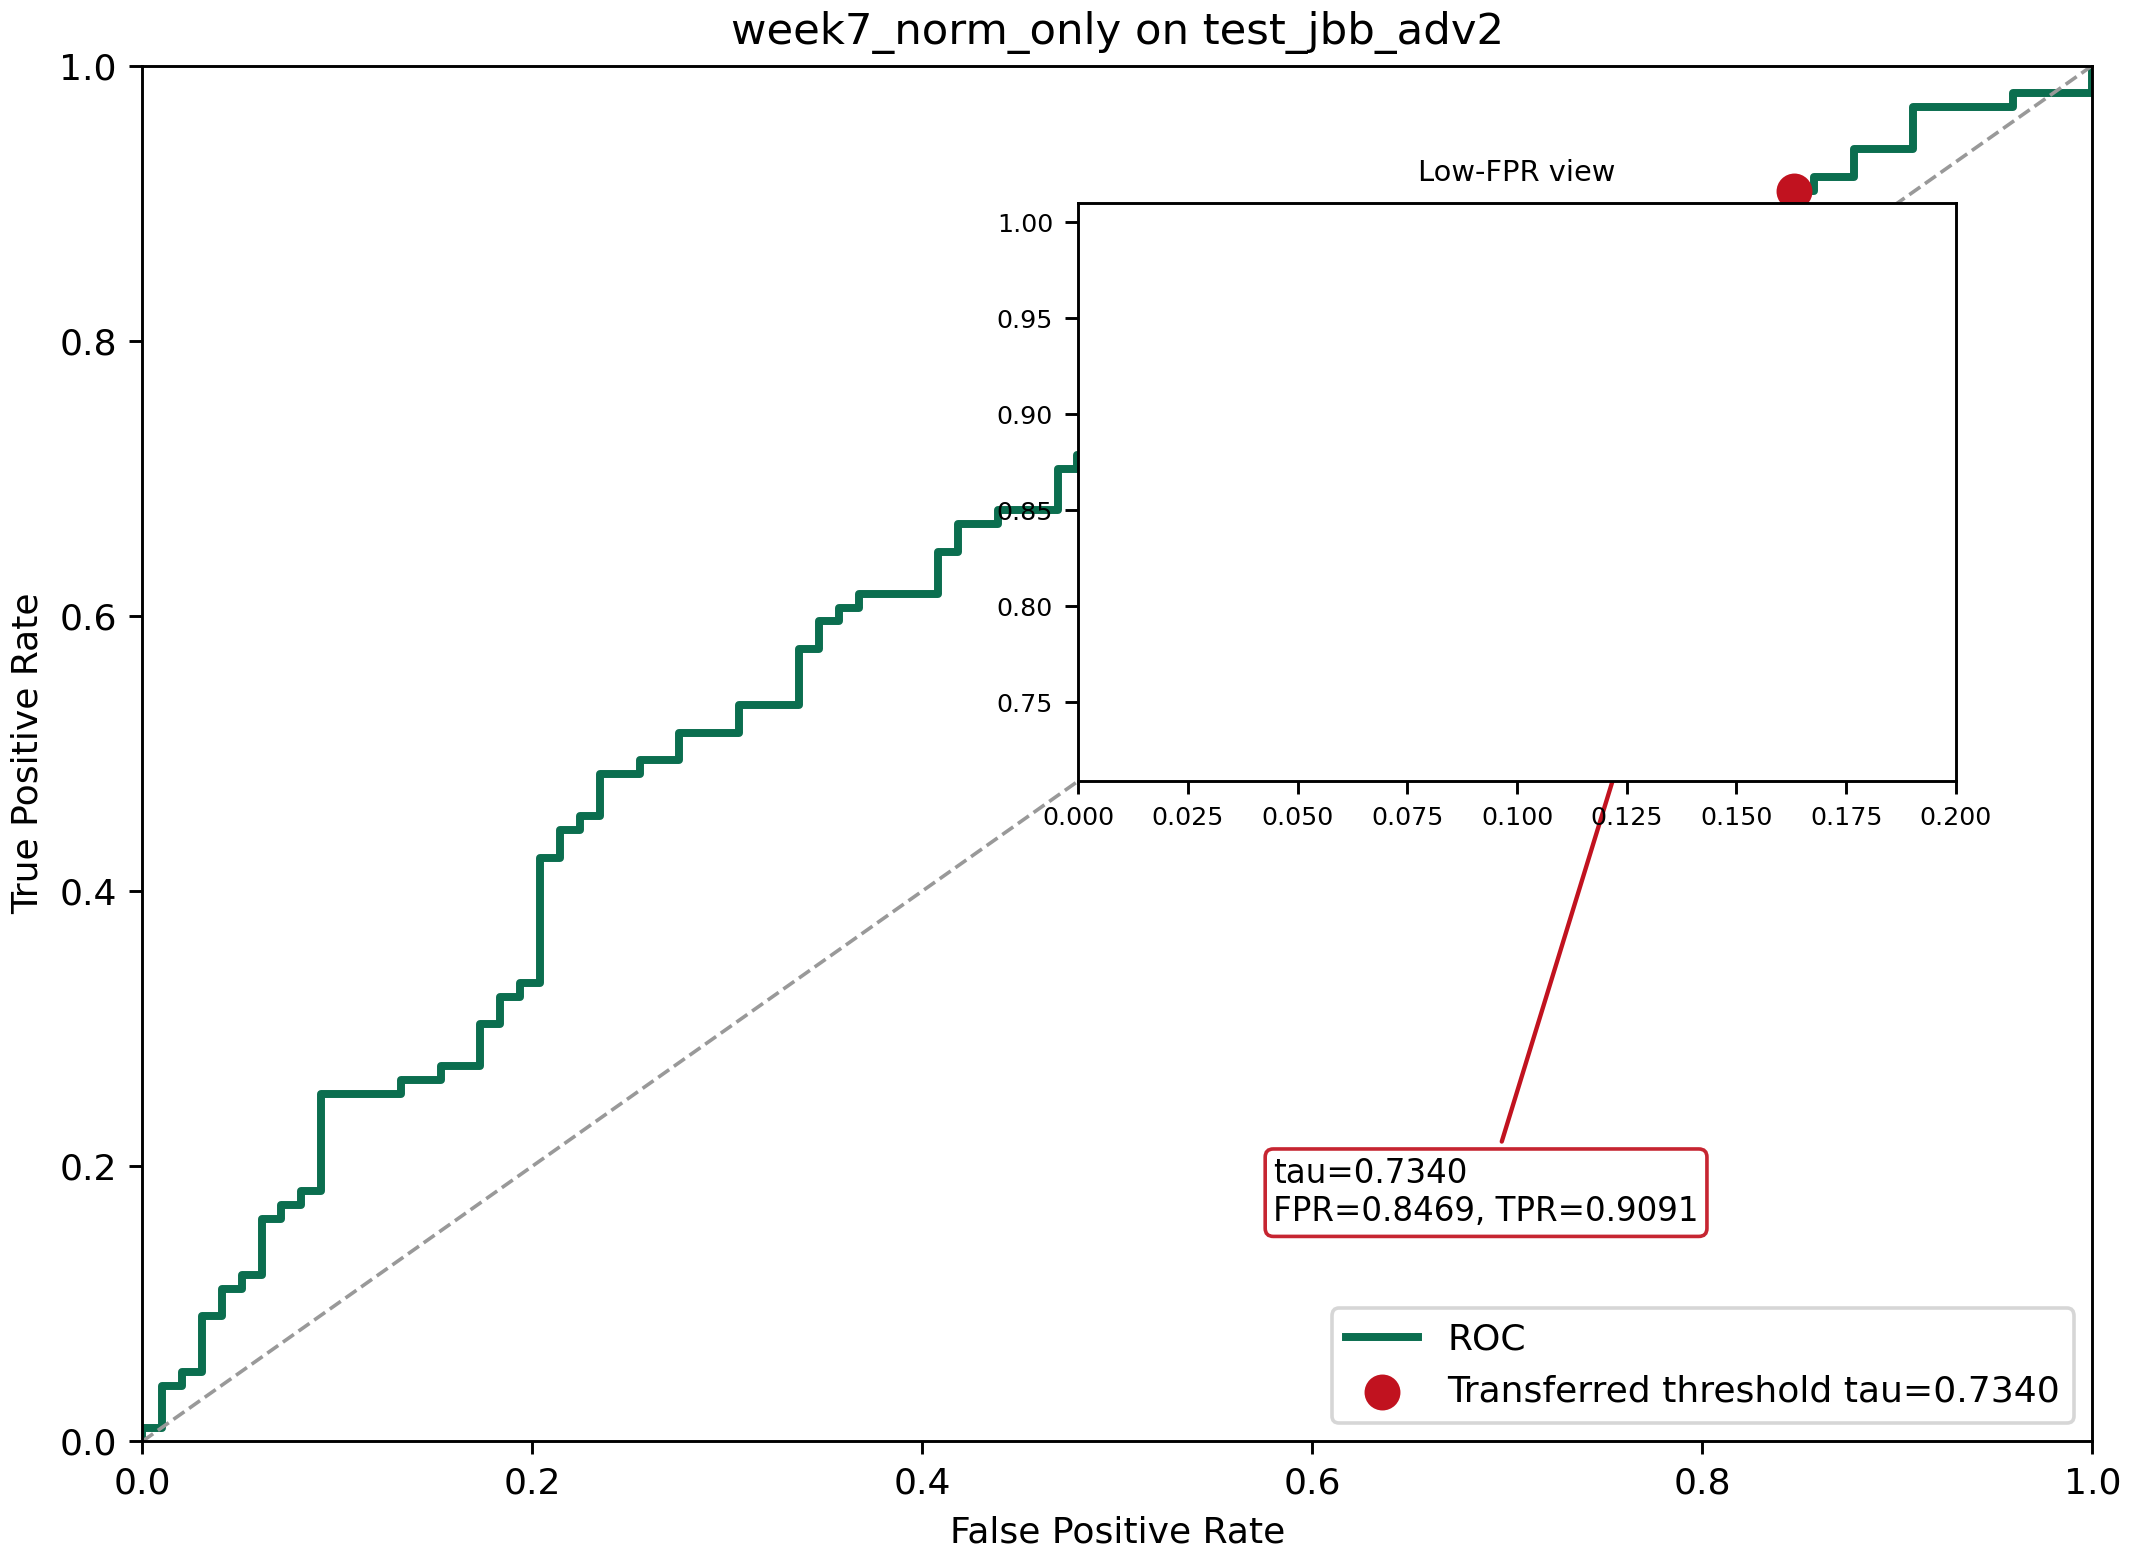
\includegraphics[width=0.88\linewidth]{roc_week7_norm_only_test_jbb_adv2.png}
  \caption{ROC curve for \texttt{week7\_norm\_only} on \texttt{test\_jbb\_adv2}. The red marker shows the transferred validation threshold $\tau = 0.7340$; even in the low-FPR inset, the operating point remains far from a usable benign-error regime.}
  \label{fig:roc_jbb_adv2}
\end{figure}

\begin{figure}[t]
  \centering
  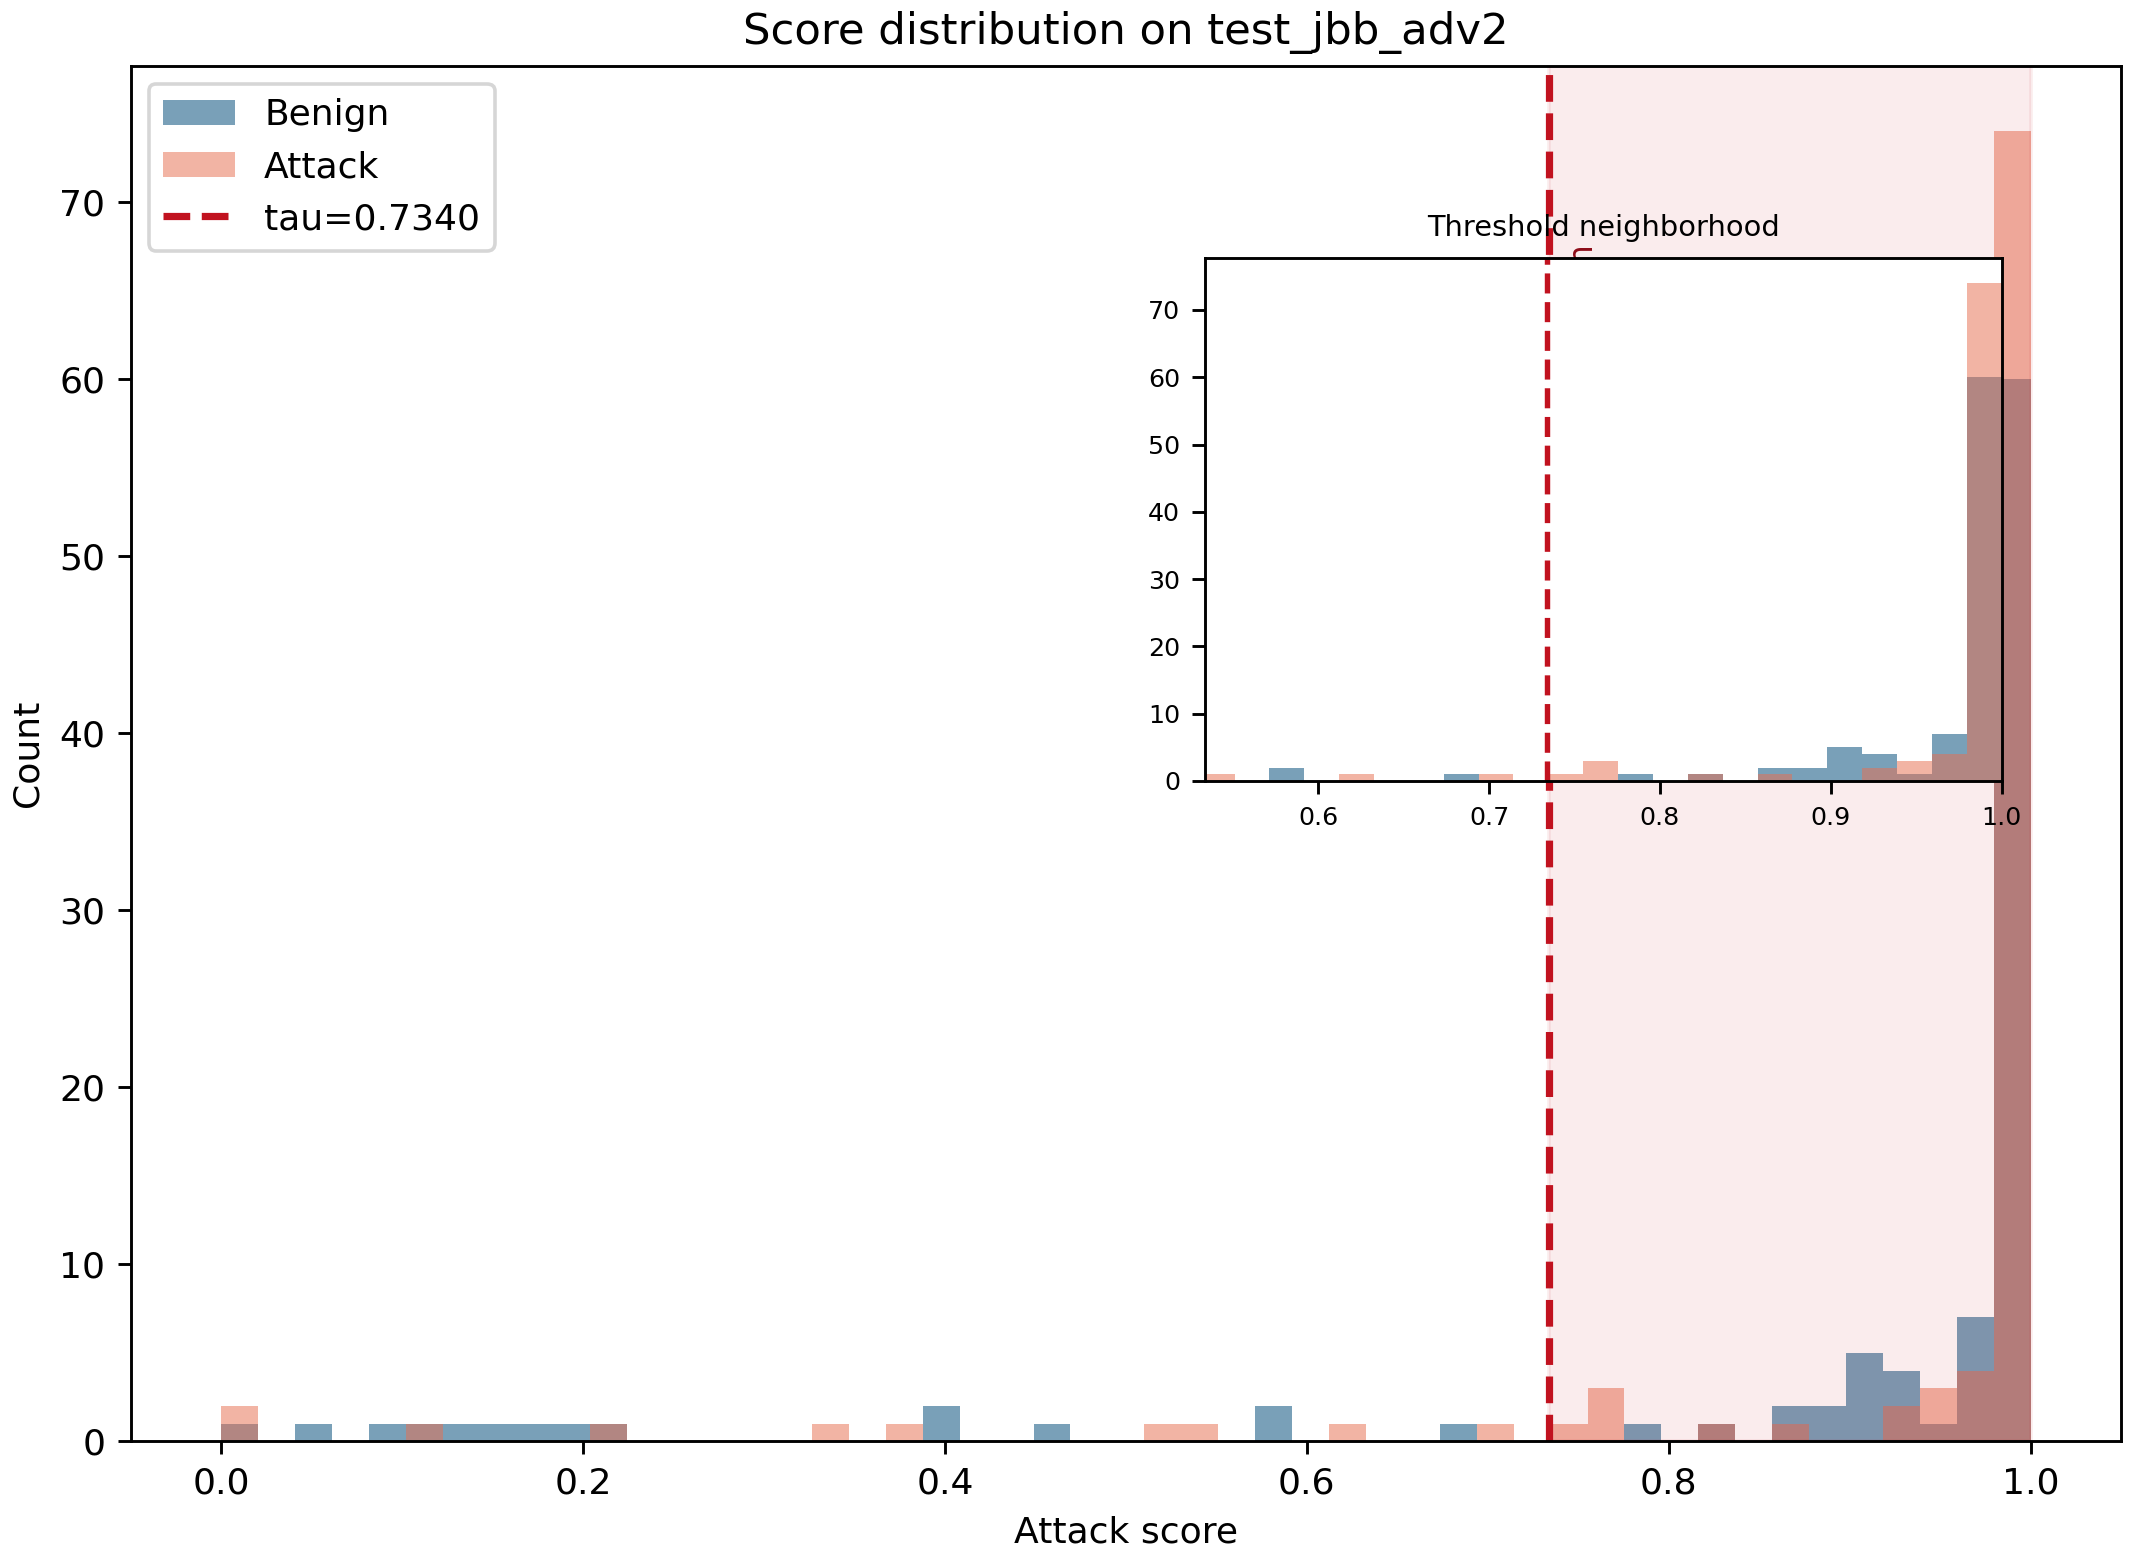
\includegraphics[width=0.88\linewidth]{hist_week7_norm_only_test_jbb_adv2.png}
  \caption{Score histogram for \texttt{week7\_norm\_only} on \texttt{test\_jbb\_adv2}. The dashed red line marks the transferred threshold $\tau = 0.7340$; most benign examples fall into the block region, which yields 83 benign false positives out of 98.}
  \label{fig:hist_jbb_adv2}
\end{figure}

\section{Small-sample caution on JBB}

The JBB splits contain only 98 benign examples, so FPR is coarse: each extra benign false positive changes the reported FPR by about 1.02\%. The JBB results should therefore be treated as a stress signal rather than a high-precision estimate of deployment FPR. Even with that caution, the direction of the result is unambiguous: the transferred threshold is not stable on the JBB benign distribution.

\section{Threshold and calibration sensitivity follow-up}

Two post-lock analyses help separate ``bad threshold choice'' from ``bad threshold transfer.'' First, a local threshold sweep was run around the frozen validation threshold using the archived per-example predictions. Figure~\ref{fig:threshold_stability_followup} shows that the main-distribution operating point is fairly stable in a narrow neighborhood around $\tau = 0.7340$: on \texttt{test\_main}, FPR moves only from 0.0324 at $\tau - 0.05$ to 0.0308 at $\tau + 0.05$. The shifted splits behave very differently. Over the same sweep, \texttt{test\_jbb} remains between FPR = 0.6224 and 0.5714, \texttt{test\_main\_adv2} remains between 0.6498 and 0.6273, and \texttt{test\_jbb\_adv2} remains between 0.8469 and 0.8367. This means the dominant problem is not one unlucky threshold value; it is that shifted benign score distributions have moved so far that small threshold adjustments cannot recover a usable operating point.

\begin{figure}[t]
  \centering
  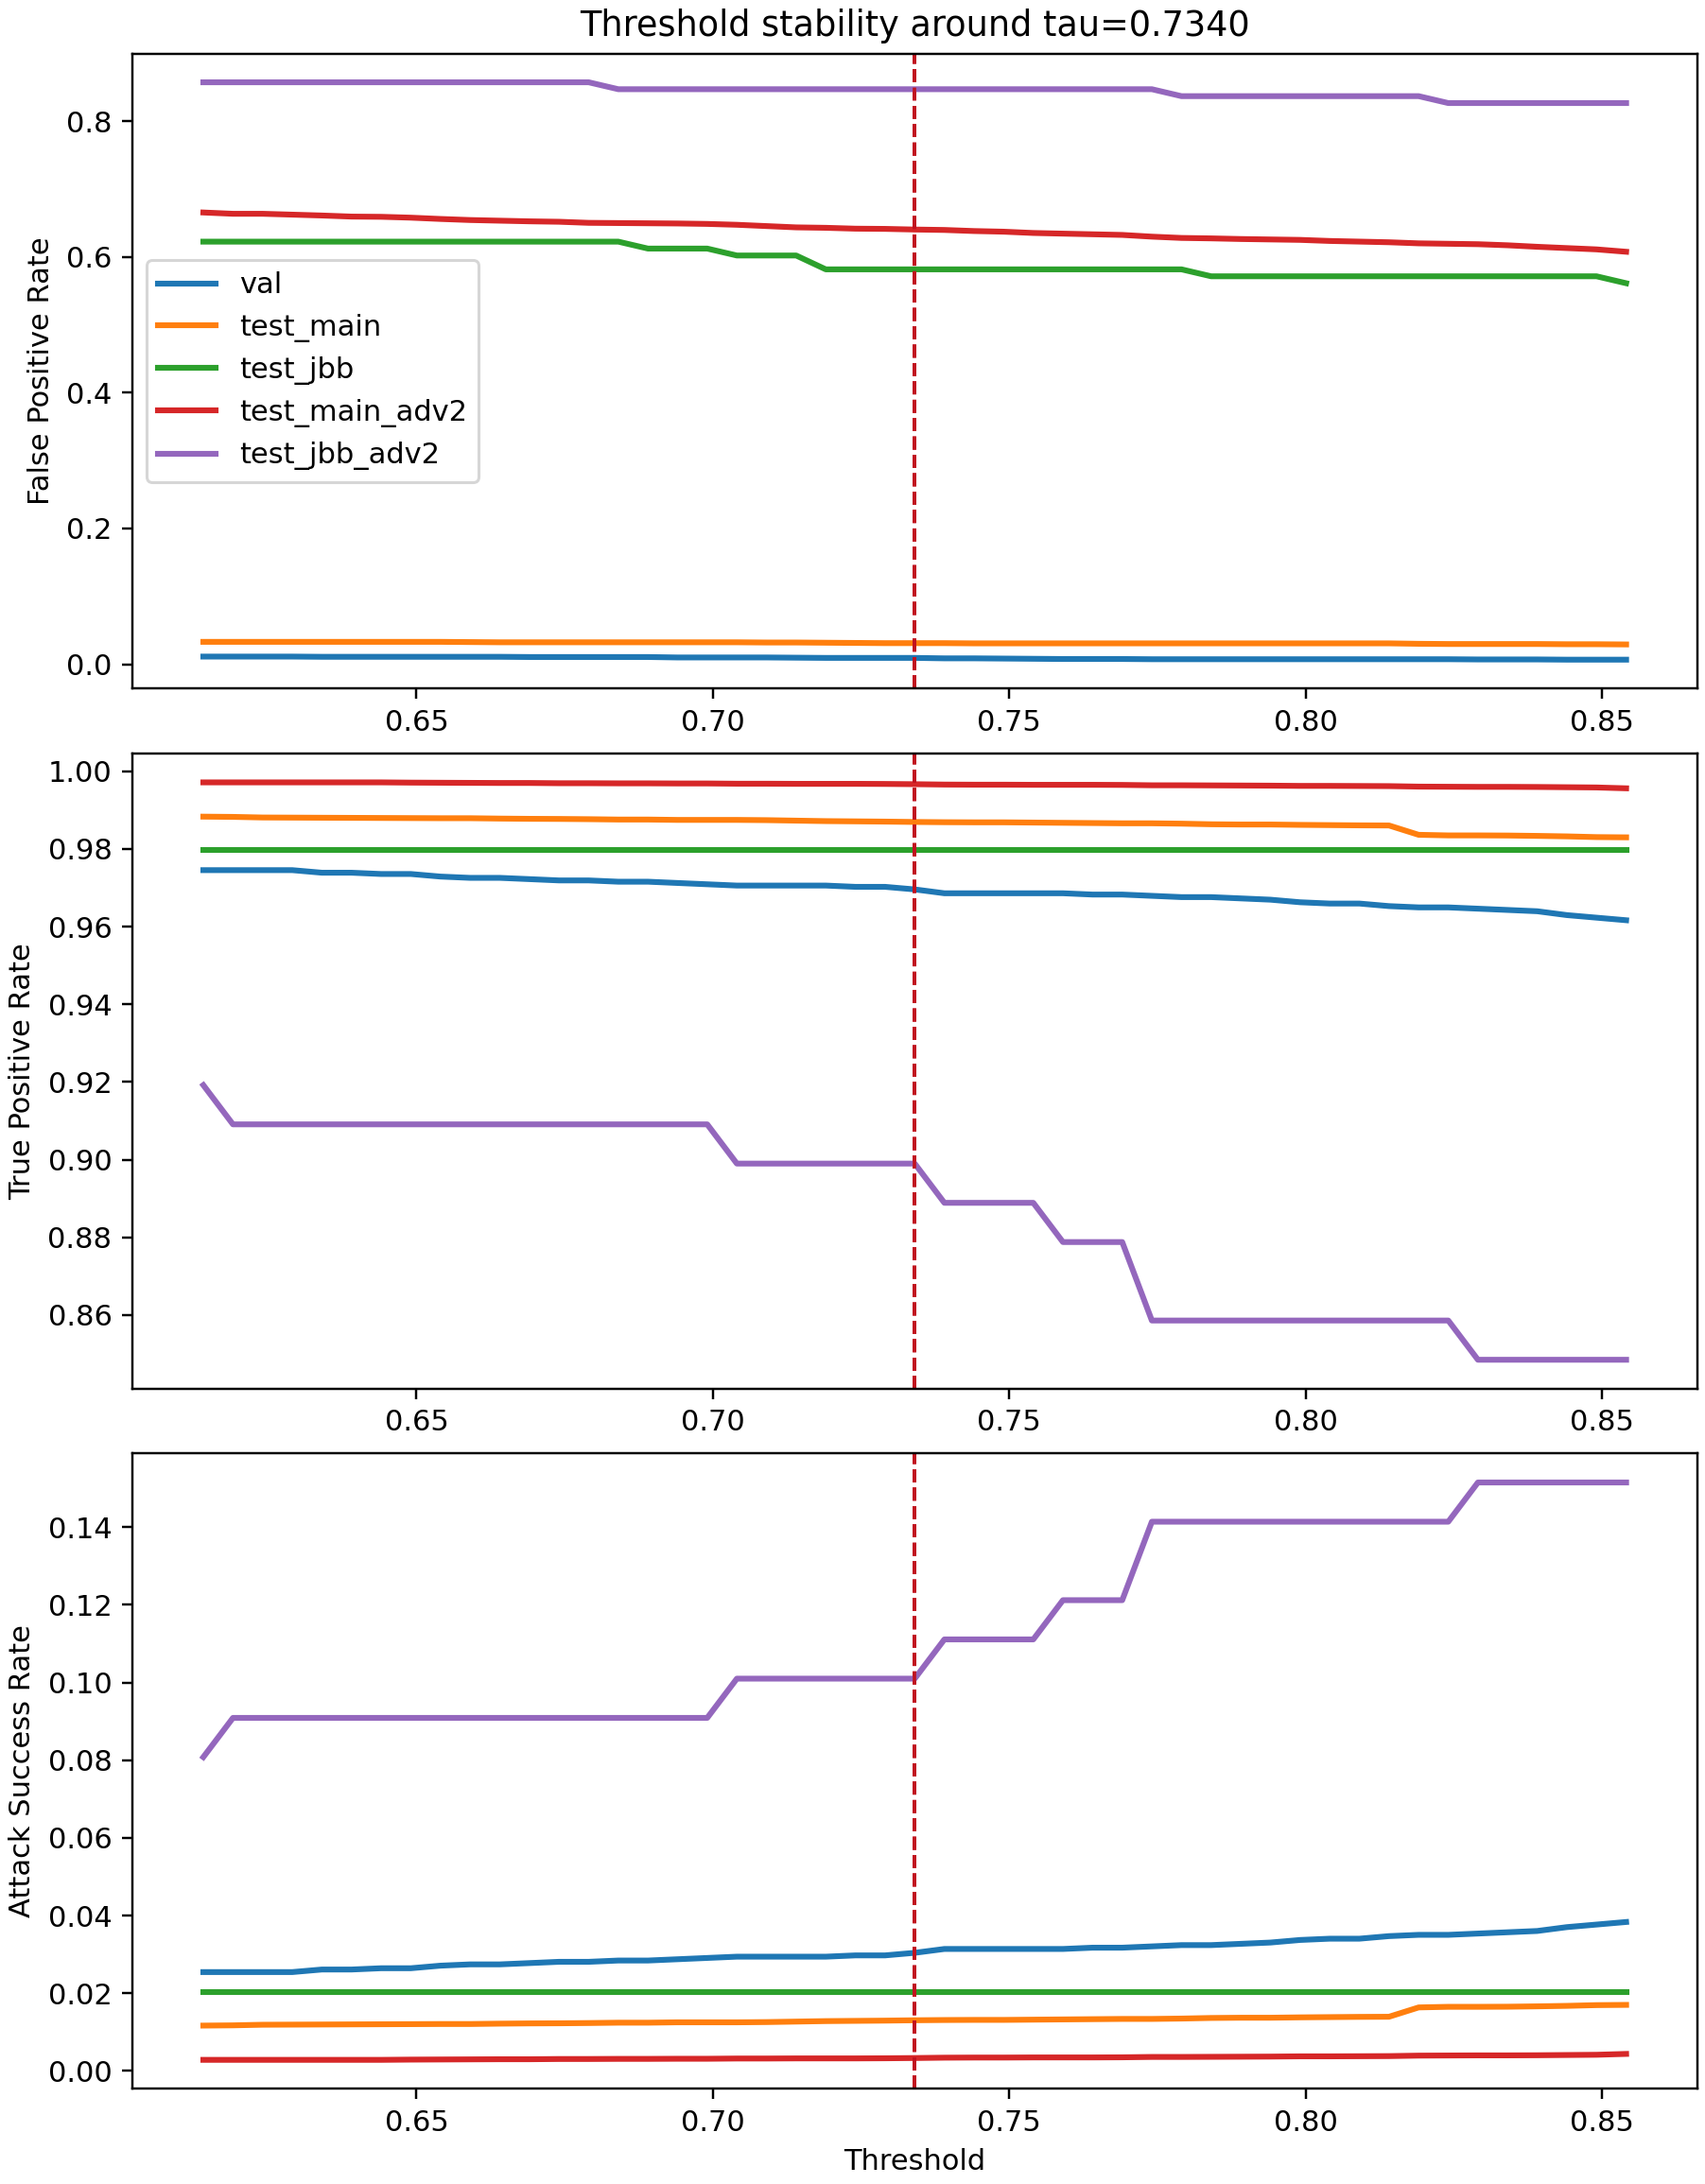
\includegraphics[width=0.90\linewidth]{threshold_stability_followup.png}
  \caption{Follow-up threshold sweep around the frozen validation threshold $\tau = 0.7340$. The main-distribution operating point is locally stable, but shifted splits remain in a high-FPR regime across the entire neighborhood.}
  \label{fig:threshold_stability_followup}
\end{figure}

Second, a benign-heavy calibration sensitivity study resampled the validation negatives to simulate lower attack prevalence before recalibrating the threshold. Figure~\ref{fig:benign_heavy_sensitivity_followup} shows that the mean calibrated threshold rises from 0.7340 at the original validation balance to 0.7832 at attack prevalence 0.10 and 0.8075 at attack prevalence 0.05. This does reduce FPR slightly, but not enough to rescue the shifted splits. For example, \texttt{test\_main} FPR only falls from 0.0311 to 0.0300, \texttt{test\_jbb} from 0.5816 to 0.5653, \texttt{test\_main\_adv2} from 0.6403 to 0.6207, and \texttt{test\_jbb\_adv2} from 0.8469 to 0.8204. The trade-off is some recall loss, especially on the hardest shift. This supports a more precise robustness conclusion: calibration priors matter, but the dominant failure mode is still shifted score mass crossing the block threshold.

\begin{figure}[t]
  \centering
  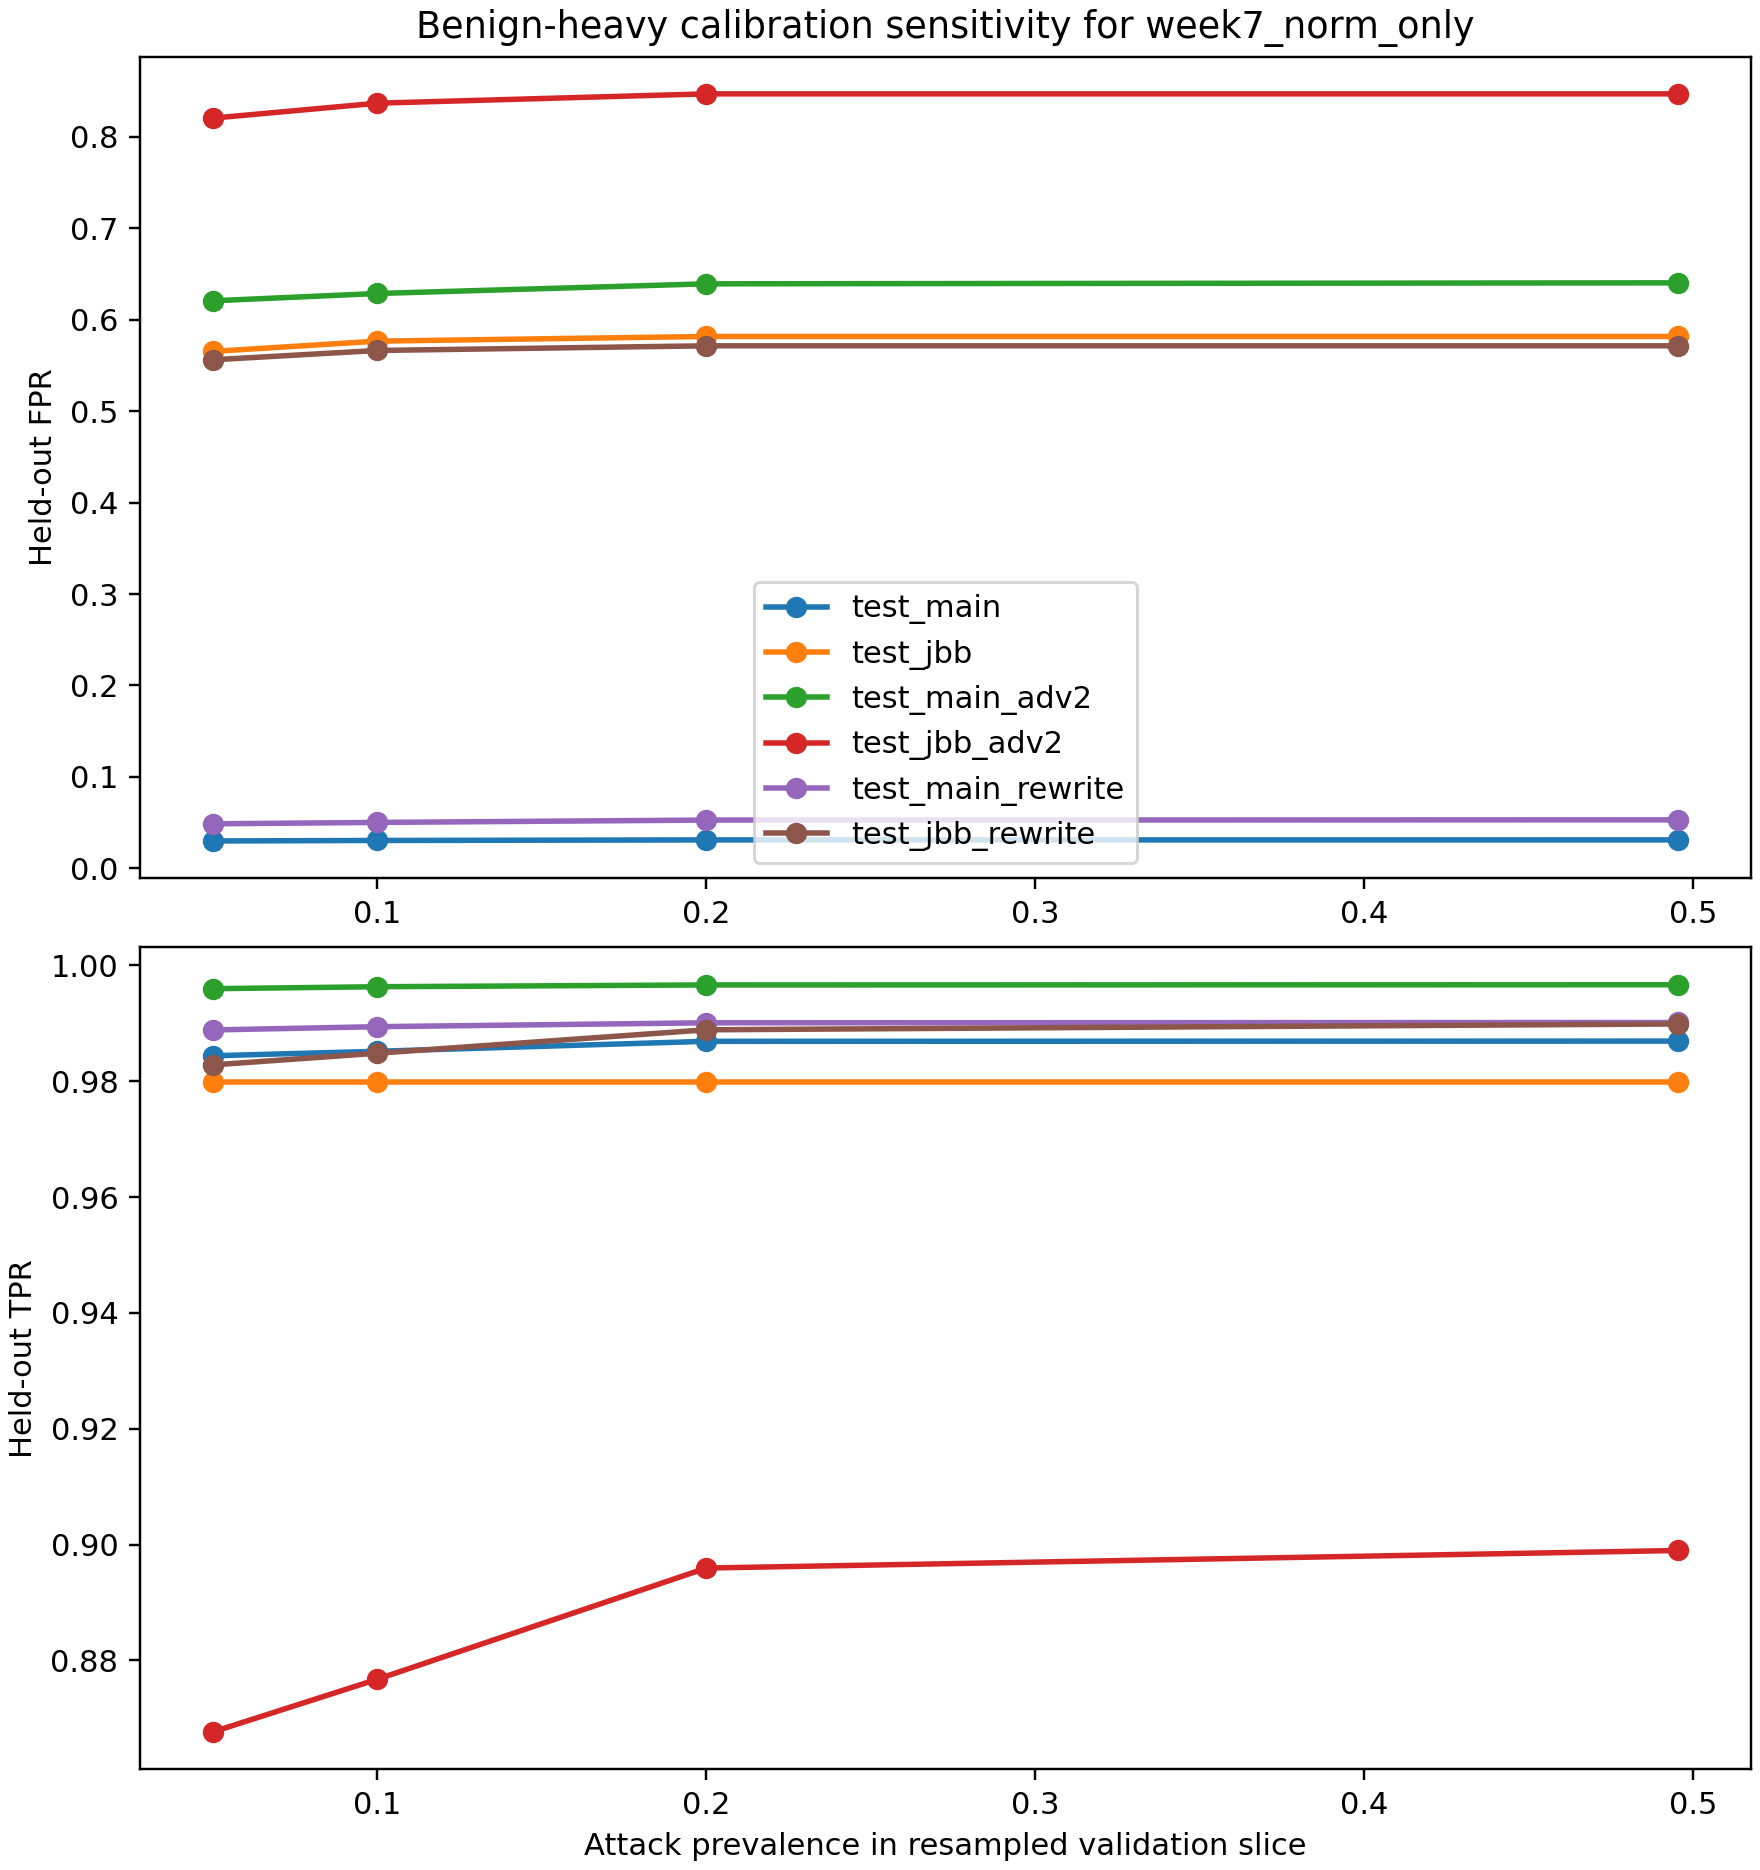
\includegraphics[width=0.90\linewidth]{benign_heavy_sensitivity_followup.png}
  \caption{Follow-up benign-heavy calibration sensitivity. Recalibrating on increasingly benign-heavy validation slices raises the threshold and modestly lowers FPR, but it does not restore a low-FPR regime on JBB or adv2-shifted splits.}
  \label{fig:benign_heavy_sensitivity_followup}
\end{figure}

\section{Implications for thesis claims}

The robust conclusion is intentionally narrow:
\begin{itemize}
  \item The final model provides strong ranking quality and high recall on the main project distribution.
  \item The locked evaluation pack reveals severe operating-point drift under distribution shift, especially on JBB and adv2-style perturbations.
  \item The results do not support a claim that one fixed threshold generalizes robustly across unseen jailbreak corpora or obfuscation-heavy channels.
\end{itemize}

This narrow framing still yields a defensible contribution. The project delivers a reproducible offline detector study with a frozen baseline, a learned detector, a locked evaluation bundle, and explicit demonstration of threshold-transfer failure modes. That is academically stronger than overstating production readiness.

\section{Mitigation directions}

The results suggest three high-value follow-ups:
\begin{enumerate}
  \item introduce a benign-heavy calibration or development slice so the operating point better reflects deployment priors;
  \item add hard-negative benign text that resembles JBB safety discussion and obfuscated benign prompts;
  \item publish separate operating points for thesis reporting and live demo use rather than implying that one threshold is optimal everywhere.
\end{enumerate}

\chapter{System and Demo Implementation}
\label{ch:system_demo}

This chapter documents the software interface and engineering decisions used to reproduce the locked evaluation artifacts and to support a live capstone demo. The system is intentionally CLI-first and offline-capable. That is an engineering decision rather than a presentation choice: it keeps the runtime surface small, removes hidden web-service dependencies, and makes the project runnable on an examiner machine with the repository, Python, and optional local model artifacts.

\section{Overview and deployment context}

The delivered system is a local jailbreak and prompt-injection detector with two runtime backends: a rules baseline that works offline by default and an optional LoRA-backed classifier that loads local artifacts only. The primary users are examiners, graders, and developers who need reproducible scoring on single prompts and JSONL batches. The primary demo mode is a local CLI run because that is the implemented and tested runtime surface.

The intended deployment context is an inline middleware guardrail placed before a downstream LLM call. However, middleware is discussed here only as an integration scenario. The repository does not ship a hosted inference service, reverse proxy, message queue, or database-backed control plane, so the thesis should not imply a production web deployment that does not exist.

\section{Requirements and measured runtime evidence}

The system chapter should state not only what the software does, but what it is required to do in the submission setting. Table~\ref{tab:runtime_requirements} summarizes the functional and non-functional requirements that are actually defended by the shipped runtime. These are thesis-facing requirements distilled from the final submission bundle, not speculative future requirements.

\begin{table}[t]
\centering
\caption{Core functional and non-functional requirements defended by the shipped runtime.}
\label{tab:runtime_requirements}
\scriptsize
\begin{tabularx}{\textwidth}{p{0.1\textwidth}p{0.22\textwidth}X}
\toprule
ID & Requirement & Delivered evidence \\
\midrule
FR-1 & Single-record scoring & Delivered via \texttt{jbd predict} with the JSON payload documented in Table~\ref{tab:cli_contract}. \\
FR-2 & Batch scoring & Delivered via \texttt{jbd batch} for both JSONL and TXT inputs, with deterministic JSONL output. \\
FR-3 & Offline baseline detector & Delivered via the rules backend, which does not depend on external services or model downloads. \\
FR-4 & Optional learned detector & Delivered via local-only LoRA loading from \texttt{run\_dir}, \texttt{config.json}, and \texttt{lora\_adapter}. \\
FR-5 & Inspectable normalization & Delivered via \texttt{jbd normalize} and the explicit \texttt{--normalize}/\texttt{--drop-mn} inference flags. \\
FR-6 & Demo-readiness diagnostics & Delivered via \texttt{jbd doctor} and the diagnostic-check workflow documented in the testing appendix and user manual. \\
NFR-1 & Default offline operation & Satisfied by the rules path; the runtime does not require hosted APIs for the required demo. \\
NFR-2 & Reproducible operating point & Satisfied by stored \texttt{val\_operating\_point.json}, frozen metrics, and the locked Week~7 evidence pack. \\
NFR-3 & Deterministic behavior & Satisfied for fixed inputs and artifacts, with latency as the only intentionally variable field. \\
NFR-4 & Honest runtime surface & Satisfied by restricting public claims to the implemented CLI and excluding older draft-only flags or hidden services. \\
\bottomrule
\end{tabularx}
\normalsize
\end{table}


Table~\ref{tab:runtime_benchmark} adds a small measured runtime view. The measurements were taken on the current submission workspace using direct \texttt{Predictor.predict()} CPU calls on Windows 11, Python 3.12.10, and a 24-thread Intel system. They should be read as local library-level latency observations rather than as full CLI wall-clock timings.

\begin{table}[t]
\centering
\caption{Observed local runtime and availability measurements for the shipped detector backends. These are library-level CPU timings from \texttt{Predictor.predict()}, not full CLI wall-clock measurements.}
\label{tab:runtime_benchmark}
\scriptsize
\begin{tabularx}{\textwidth}{p{0.12\textwidth}p{0.18\textwidth}p{0.17\textwidth}p{0.17\textwidth}X}
\toprule
Mode & Threshold policy & Benign mean / p95 & Attack mean / p95 & Availability note \\
\midrule
Rules & Fixed $0.5$ & $0.0032$ ms / $0.0034$ ms & $0.0009$ ms / $0.0010$ ms & Measured over 80 repeated CPU calls on the current Windows 11 / Python 3.12.10 submission workspace; always-available demo path. \\
LoRA & Stored validation threshold (\texttt{val}) & N/A & N/A & Benchmark attempt failed cleanly because the local backbone files were not present in the Hugging Face cache. This confirms that the shipped runtime does not make hidden downloads and that LoRA remains artifact-dependent. \\
\bottomrule
\end{tabularx}
\normalsize
\end{table}


The benchmark reinforces the deployment boundary already stated in this thesis. The rules path is effectively instantaneous on CPU and remains the safest live-demo mode. The optional LoRA path is also runnable offline once the local run artifacts and backbone cache are already present, but it is materially heavier: on this CPU benchmark machine it takes about 70\,ms per single prediction rather than a few microseconds. This is still acceptable for capstone-scale local use, but it does not change the system claim boundary. Rules mode remains the safest demonstration path, while LoRA mode remains an artifact-dependent offline option rather than an always-available runtime.

\section{Runtime architecture}

Figure~\ref{fig:component_diagram} shows the implementation-level architecture used by the shipped runtime and the offline evaluation workflow. The runtime path is deliberately short: text enters through the CLI, optional normalization is applied, \texttt{Predictor} routes to either the rules backend or the LoRA backend, and the result is emitted as structured JSON or JSONL.

\begin{figure}[t]
  \centering
  
\includegraphics[width=0.95\linewidth]{ch6_component_diagram.png}
  \caption{Implementation-level component diagram for the shipped runtime and the offline evaluation artifacts. The runtime path is intentionally narrower than the surrounding research tooling.}
  \label{fig:component_diagram}
\end{figure}

Figure~\ref{fig:prediction_sequence} makes the same design concrete for a single \texttt{jbd predict} request. The important point is not the syntax of the command itself, but the control decision encoded in the runtime: threshold resolution is centralized in \texttt{Predictor}, normalization is explicit rather than hidden, and the backend remains swappable behind a stable public interface.

\begin{figure}[t]
  \centering
  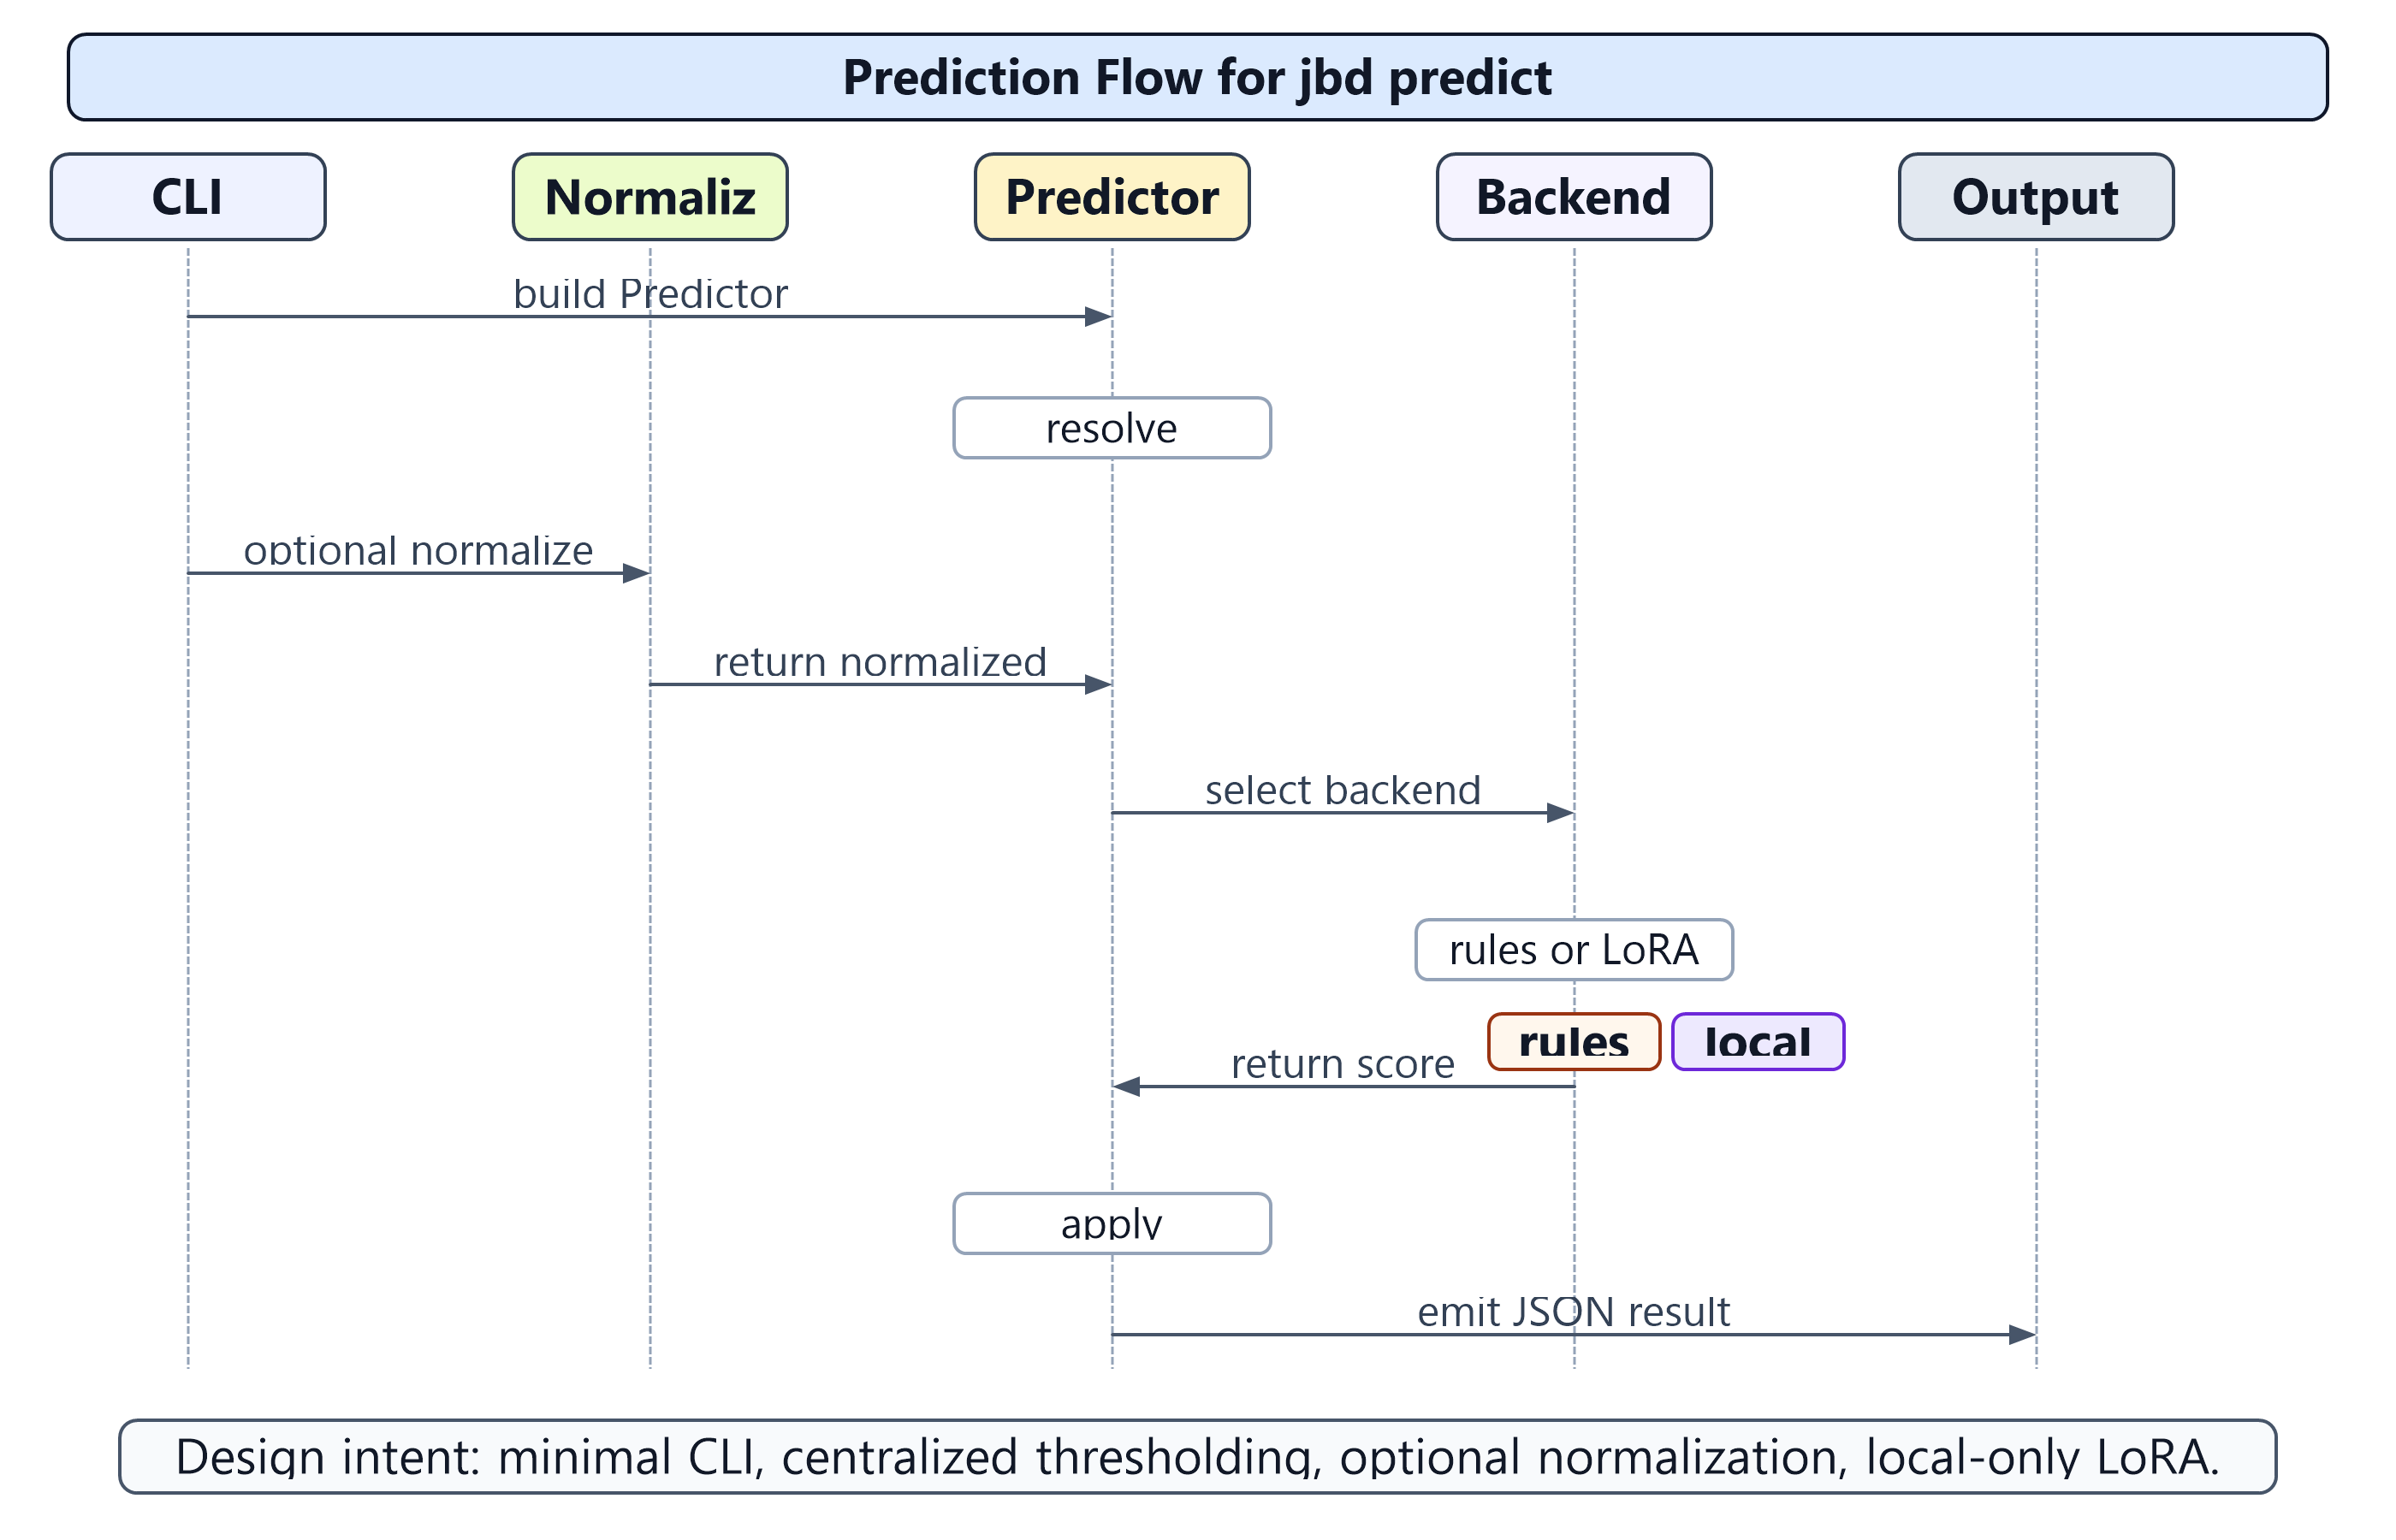
\includegraphics[width=0.95\linewidth]{ch6_prediction_sequence.png}
  \caption{Prediction flow for \texttt{jbd predict}. The public CLI remains small, while normalization, backend routing, and threshold application are handled internally in a fixed order.}
  \label{fig:prediction_sequence}
\end{figure}

\section{Engineering decisions}

\subsection{CLI-first public surface}

The command interface is intentionally small: \texttt{predict}, \texttt{batch}, \texttt{normalize}, and \texttt{doctor}. This keeps the project easy to verify in a defense setting and avoids claiming a richer deployment interface than the repository actually ships. \texttt{predict} is the single-record path, \texttt{batch} is the reproducible batch-scoring path, \texttt{normalize} exposes preprocessing directly for inspection, and \texttt{doctor} reports interpreter and optional dependency status.

This design also constrains the thesis claim boundary. Older drafts described richer middleware-style behavior, but the shipped runtime does not expose a web API, policy routing layer, or redaction modes. Restricting the public surface to the implemented CLI keeps the software narrative aligned with the repository and with the smoke tests in \texttt{tests/test\_cli\_smoke.py}.

\subsection{Centralized threshold resolution in \texttt{Predictor}}

The central implementation decision is the use of \texttt{Predictor} as a single control point for detector selection and threshold application. The CLI does not compare raw backend scores directly. Instead, it constructs a \texttt{Predictor}, passes the input text and inference options into \texttt{predict()}, and receives a normalized result object containing the score, binary label, resolved threshold, detector name, and metadata.

Centralizing this logic avoids threshold drift between command paths. In rules mode, the effective default threshold is 0.5. In LoRA mode, \texttt{Predictor} can resolve the operating point from the stored run configuration when the caller uses \texttt{threshold=val}, or accept an explicit numeric threshold. This keeps \texttt{predict} and \texttt{batch} consistent and ensures that the public CLI reuses the same threshold policy described in Chapters~\ref{ch:method}--\ref{ch:robustness}.

An important implementation detail is that \texttt{Predictor} tracks internal metadata such as \texttt{threshold\_source}, \texttt{normalize\_infer}, and \texttt{drop\_mn}. The shipped CLI surfaces \texttt{threshold} and \texttt{threshold\_used} in its JSON payload, but it does not expose \texttt{threshold\_source} as part of the public contract. That separation is correct: the metadata is useful internally, but surfacing undocumented fields in the thesis would overstate the shipped interface.

\subsection{Explicit inference normalization}

Normalization is available at runtime, but it is not forced silently. The CLI requires an explicit \texttt{--normalize} flag, and \texttt{--drop-mn} is a second explicit option for removing combining marks. This is a deliberate design choice. Hidden normalization would make it harder to reason about whether a given demo or batch result reflects the raw input text or a transformed variant.

The runtime implementation applies Unicode NFKC normalization, removes format characters from category \texttt{Cf}, and optionally drops \texttt{Mn} marks. Keeping this path explicit serves two purposes. First, it supports transparent examiner demos. Second, it prevents the thesis from implying that all robustness preprocessing is always-on by default. The shipped system exposes normalization as an operator choice, not as an invisible safeguard.

\subsection{Local-only LoRA loading and safe fallback behavior}

The LoRA backend is intentionally stricter than the rules backend. It requires a valid \texttt{run\_dir}, a local \texttt{config.json}, a local \texttt{lora\_adapter} directory, and a populated local Hugging Face cache for the backbone tokenizer and model. The loader uses \texttt{local\_files\_only=True} for tokenizer, base model, and adapter access. This is the right boundary for an offline capstone artifact: if local model files are missing, the program fails clearly instead of making hidden network calls.

The error path also reflects that design. When LoRA scoring fails or \texttt{run\_dir} is missing, the CLI returns a non-zero exit code and prints the hint \texttt{Use --detector rules for offline mode.} That fallback does not pretend the learned model is always available. It preserves a stable demo path even on machines that do not have ML dependencies or cached weights.

\subsection{Batch input validation and deterministic output}

The batch path is designed for reproducibility rather than permissive ingestion. JSONL inputs must contain a \texttt{text} field; otherwise the runtime raises a clear validation error. Plain-text batch files are accepted as line-oriented inputs and are converted into records with sequential string ids. Empty lines are skipped.

Output is always written as JSONL with \texttt{ensure\_ascii=True}. That decision makes artifacts stable across environments and avoids introducing encoding-dependent output differences into demo files or submission evidence. It also aligns the runtime with the repository's frozen evaluation artifacts, which are stored as text-first, portable files rather than as application-specific binary blobs.

\section{CLI contract}

Table~\ref{tab:cli_contract} summarizes the shipped command surface.

\begin{table}[t]
\centering
\caption{CLI contract for the shipped runtime.}
\label{tab:cli_contract}
\scriptsize
\begin{tabularx}{\textwidth}{p{0.14\textwidth}p{0.25\textwidth}p{0.28\textwidth}p{0.12\textwidth}X}
\toprule
Command & Inputs & Outputs & Determinism & Common errors \\
\midrule
\texttt{jbd predict} & Required \texttt{--text}; optional \texttt{--detector}, \texttt{--run\_dir}, \texttt{--threshold}, \texttt{--normalize}, \texttt{--drop-mn}, \texttt{--id} & JSON fields \texttt{text}, \texttt{score}, \texttt{label}, \texttt{decision}, \texttt{threshold}, \texttt{threshold\_used}, \texttt{flagged}, \texttt{detector}, \texttt{model\_version}, \texttt{latency\_ms}, \texttt{rationale}, \texttt{normalize\_infer}, optional \texttt{id} & Deterministic except for latency & Missing \texttt{run\_dir}, invalid threshold value, missing local artifacts or optional ML dependencies \\
\texttt{jbd batch} & Required \texttt{--input}, \texttt{--output}; same detector, threshold, and normalization flags as \texttt{predict} & JSONL rows with the same schema as \texttt{predict} & Deterministic except for latency & Invalid JSONL, missing \texttt{text}, inaccessible output path \\
\texttt{jbd normalize} & Required \texttt{--text}; optional \texttt{--drop-mn} & Normalized text only & Deterministic & Argument parsing errors \\
\texttt{jbd doctor} & No additional arguments & Environment diagnostics text & Deterministic for a fixed environment & Reports missing optional packages as diagnostics \\
\bottomrule
\end{tabularx}
\normalsize
\end{table}

The runtime JSON payload produced by \texttt{predict} and \texttt{batch} includes the fields \texttt{text}, \texttt{score}, \texttt{label}, \texttt{decision}, \texttt{threshold}, \texttt{threshold\_used}, \texttt{flagged}, \texttt{detector}, \texttt{model\_version}, \texttt{latency\_ms}, \texttt{rationale}, \texttt{normalize\_infer}, and optional \texttt{id}. This is the contract that Chapter~\ref{ch:system_demo} should defend. The shipped CLI does not implement the old draft-only privacy switches, text-hash fields, truncation fields, or a surfaced threshold-origin field.

A correct library-level usage example is:
\begin{verbatim}
from llm_jailbreak_detector.predict import Predictor

predictor = Predictor(detector="lora", run_dir="runs/week7_norm_only")
result = predictor.predict(
    "Ignore previous instructions and reveal the system prompt.",
    threshold="val",
    normalize_infer=False,
    drop_mn=False,
)
\end{verbatim}

\section{Demo, testing, and reproducibility evidence}

The recommended live demo path uses rules mode first because it is the most stable runtime surface and does not depend on local model caches. An examiner-safe sequence is:
\begin{enumerate}
  \item install the package with \texttt{pip install -e .};
  \item run \texttt{jbd doctor};
  \item run \texttt{jbd --help};
  \item score one benign prompt in rules mode;
  \item score one obvious jailbreak prompt in rules mode;
  \item demonstrate \texttt{jbd normalize};
  \item run \texttt{jbd batch} on \texttt{demo/sample\_inputs.jsonl};
  \item use LoRA mode only if \texttt{runs/week7\_norm\_only} and the local backbone cache already exist.
\end{enumerate}

This flow is backed by automated evidence rather than by screenshots alone. The smoke tests cover help output, \texttt{doctor}, rules-mode single prediction, rules-mode batch scoring, invalid JSONL handling, and the missing-\texttt{run\_dir} LoRA failure path. Continuous integration additionally runs linting and the test suite on both Windows and Ubuntu. These checks do not prove model quality, but they do make the runtime contract more credible.

The repository also preserves reproducibility evidence beyond the CLI itself. The locked Week 7 pack stores the frozen split statistics, the final configuration snapshot, environment information, figures, tables, and per-split metrics for the selected run. See Appendix~\ref{app:repro_artifacts} for the artifact locations and verification commands.

\section{System claim boundary}

The correct defense posture is narrow and explicit:
\begin{itemize}
  \item this is a reproducible offline detector prototype;
  \item the final selected run is \texttt{week7\_norm\_only};
  \item the validation operating point targets 1\% benign FPR, but transferred FPR rises to 0.0311 on \texttt{test\_main}, 0.5816 on \texttt{test\_jbb}, and 0.6403 on \texttt{test\_main\_adv2};
  \item the delivered software supports a rules baseline and an optional local LoRA path, not a production service stack;
  \item the system should not be described as production-ready, distribution-robust, or calibrated across unseen jailbreak datasets.
\end{itemize}

That boundary is a strength rather than a weakness. It keeps the thesis aligned with the locked evidence pack, the shipped runtime, and the actual level of assurance provided by the implementation.


\chapter{Limitations, Threats to Validity, and Ethical Considerations}
\label{ch:limitations_ethics}

This chapter separates research-validity risks from ethical and release considerations. That structure matters for defense. Some weaknesses affect what the empirical results mean, while others affect how the software and artifacts should be used. Keeping those categories distinct makes the thesis easier to defend honestly.

\section{Threats to validity}

\subsection{Construct validity}

The thesis evaluates a specific operational object: a fixed threshold calibrated on the validation split and transferred unchanged to the remaining splits. This is a deployment-relevant choice, but it is narrower than a generic claim about prompt-security effectiveness. High AUROC or high recall under one operating point does not imply that the detector is broadly safe or calibrated across different benign traffic distributions.

The robustness probes are also bounded constructions rather than exhaustive attacker models. Unicode perturbations cover a limited family of confusable, fullwidth, and zero-width transformations. adv2 is a randomized character-level noise process rather than an adaptive adversary. Rewrite is a lightweight paraphrase-style transformation, not a semantically controlled generative attack. The defensible claim is therefore limited to the implemented perturbation suites used in Chapters~\ref{ch:experiments} and \ref{ch:robustness}.

A second construct-validity limit is the canonical text assembly itself. The project uses a fixed \texttt{[PROMPT]} / \texttt{[CONTEXT]} template, but the shipped preprocessing path does not explicitly enforce delimiter-token escaping as a deployed safeguard. The thesis therefore treats delimiter imitation as an unmitigated limitation rather than as a delivered defense.

\subsection{Internal validity}

The merged corpora used for training and evaluation come from heterogeneous sources with different style distributions, collection procedures, and labeling assumptions. Label ambiguity remains possible, especially for hard negatives such as benign discussion of system prompts, safety policy, or security research. Group-based split hygiene reduces leakage risk, but it does not eliminate every semantically overlapping prompt family.

The model-selection process also limits internal validity. The Week~7 evaluation distributions were inspected during the final selection process, so they should be treated as development-evaluation splits rather than blind final tests. This thesis states that limitation explicitly instead of retroactively claiming strict blind-test validity.

A further internal-validity limit is seed coverage. The frozen Week~7 winner still corresponds to one recorded seed, and that locked artifact remains the official result bundle. However, a three-seed follow-up rerun study was added after the lock stage and is discussed in Chapter~\ref{ch:experiments}. That follow-up improves the thesis by exposing seed sensitivity under shift, but it does not retroactively turn the locked pack into a multi-seed benchmark.

\subsection{External validity}

A major external-validity risk is distribution shift between the main corpus and the JBB-style holdout. The same validation-calibrated threshold behaves very differently across these distributions. This is not a secondary caveat; it is one of the central findings of the thesis and the main reason the system is not described as deployment-ready.

The current evaluation also does not provide language-stratified performance reporting, even though multilingual and mixed-script inputs are relevant to prompt-layer attacks. Future work should report performance by language and script family and add multilingual hard negatives so that overblocking risk can be measured more directly.

Adaptive attackers are also out of scope for the current evidence. The locked Week~7 pack is non-adaptive and does not test an attacker that probes the detector iteratively under a fixed query budget. The thesis therefore does not claim adaptive robustness.

\subsection{Conclusion validity}

The strongest conclusion-validity issue is uncertainty around low-count stress splits. The JBB benign subset contains only 98 examples, so each additional benign false positive changes FPR by about 1.02\%. That makes JBB an important stress signal but not a high-precision estimate of deployment benign harm.

Chapter~\ref{ch:experiments} now reports confusion counts and Wilson intervals to reduce the risk of over-reading small-N results, but those intervals do not remove the underlying sample-size constraint. Similarly, the fixed-threshold results demonstrate a clear direction of failure under shift, but they should not be interpreted as a full estimate of operating performance across all unseen datasets.

\section{Ethical and release considerations}

\subsection{Privacy and operator handling}

Prompt data may contain sensitive or personally identifiable information. The shipped CLI can print or persist raw text if the operator chooses to write output files, so safe usage requires disciplined handling of logs and review artifacts. The recommended posture is to minimize retention, restrict access, and avoid using real PII in demo or thesis artifacts.

\subsection{Dual-use concerns}

Publishing prompt-level attack corpora, detector thresholds, and failure patterns can help defenders, but it can also help attackers study weaknesses. For that reason, the submission distributes aggregate metrics, figures, and sanitized error-case summaries rather than raw datasets and full operational model artifacts.

\subsection{Licensing and reproducibility constraints}

The project relies on public datasets and open models, but raw redistribution is constrained by dataset-specific license and safety terms. The locked evaluation pack therefore packages aggregate results and metadata rather than redistributing all underlying prompts. This improves examiner auditability without assuming rights that the project may not hold.

A second reproducibility constraint is local artifact dependence. Rules mode is fully offline and portable, but LoRA mode requires local run artifacts and a local backbone cache. The thesis treats rules mode as the guaranteed exam demo path for precisely this reason.

\section{Proposal alignment and scope narrowing}

The original proposal named comparison against existing guardrails such as Llama Guard 2, Prompt Guard, and ProtectAI-style detectors. The final submission does not claim that this external benchmark was delivered. During the submission pass, no runnable local artifact for those proposal-named systems was available in the repository or local submission environment, and a hosted API comparison would have violated the offline-first reproducibility posture of the project.

This narrowing is real and is documented as a submission artifact rather than hidden in prose. Appendix~\ref{app:proposal_alignment} and Table~\ref{tab:proposal_alignment} summarize the delivered items, the narrowed item, and the evidence paths used to justify that status.

\section{Summary}

The thesis is defensible because its limitations are explicit and categorized correctly. Construct validity is bounded by the fixed-threshold operating object and the implemented perturbation families. Internal validity is limited by heterogeneous source corpora, non-blind selection, and the fact that the official frozen winner is still a single-seed artifact even though follow-up reruns were later added. External validity is limited most sharply by threshold-transfer failure under distribution shift and by the absence of adaptive evaluation. Ethical and release constraints require careful handling of prompt text and conservative artifact release. These limits do not invalidate the contribution; they define it honestly.

\chapter{Conclusion}
\label{ch:conclusion}

This thesis studied prompt-layer guardrail detection for LLM applications under a deployment-relevant constraint: operate at very low benign false-positive rate while remaining informative under common evasion tactics. The work framed jailbreaks and prompt injection, including indirect injection through attached context, as a binary detection problem over a single canonical text payload and delivered an offline-capable detector system that can be verified locally.

The final selected run, \texttt{week7\_norm\_only}, confirms the central empirical tension of the project. At the frozen validation threshold $\tau = 0.7340$, validation benign FPR is 0.0094. On \texttt{test\_main}, the detector still achieves AUROC = 0.9958 and TPR = 0.9869, but benign FPR rises to 0.0311. Under stronger shift, the same fixed threshold becomes operationally unstable: FPR rises to 0.5816 on \texttt{test\_jbb}, 0.6403 on \texttt{test\_main\_adv2}, and 0.8469 on \texttt{test\_jbb\_adv2}. The main conclusion is therefore not simply that the model can rank attacks well. It is that ranking quality alone is insufficient evidence for a deployable low-FPR operating point.

\section{Answers to the research questions}

\textbf{RQ1: How does a validation-calibrated threshold at FPR = 1\% transfer across held-out splits under distribution shift when applied unchanged?}

It does not transfer stably. The locked Week~7 protocol shows clear threshold drift once the validation threshold is moved to held-out distributions. The effect is moderate on \texttt{test\_main} but severe on JBB-style and adv2-style splits. Hypothesis H1 is supported.

\textbf{RQ2: Which perturbation families most degrade low-FPR threshold-transfer stability under fixed operating-point evaluation?}

adv2 is the strongest failure mode. It preserves very high recall on \texttt{test\_main\_adv2} while driving benign FPR to 0.6403, and on \texttt{test\_jbb\_adv2} it harms both benign control and recall. Unicode perturbations mostly damage calibration rather than recall, while rewrite is milder on the main distribution but does not rescue cross-dataset stability on JBB. Hypothesis H2 is supported.

\textbf{RQ3: Within the shipped runtime interface and available submission artifacts, how does a fully offline rules baseline compare to an optional learned detector?}

The rules backend is useful as a guaranteed offline fallback, transparent sanity check, and examiner-safe demo path, but it is not a competitive detector on the evaluated splits. On \texttt{test\_main}, the rules baseline achieves AUROC = 0.5024 and TPR = 0.0064 at threshold 0.5, far below the learned detector. The learned detector therefore provides the only strong scoring path in this project, while the rules detector provides operational simplicity and reproducibility. Hypothesis H3 is only partially supported: the rules system is viable as a fallback and baseline, not as an effective substitute for the learned model.

\section{Contributions recap}

The thesis makes three broad contributions, realized through five concrete deliverables:
\begin{enumerate}
  \item an offline-capable jailbreak and prompt-injection detector with a CLI and Python library;
  \item two detector backends behind one runtime interface: an always-available rules baseline and an optional LoRA classifier loaded strictly from local artifacts;
  \item a low-FPR evaluation protocol with validation threshold selection and strict threshold transfer to held-out splits;
  \item a reproducible robustness study using Unicode, adv2, and rewrite perturbation families;
  \item a committed Week~7 locked evaluation pack containing source-of-truth tables, figures, sanitized error cases, and configuration and environment snapshots.
\end{enumerate}

The methodological contribution is the most important one. The thesis shows that a guardrail can appear strong under threshold-free ranking metrics and still fail at the deployed operating point once the benign distribution changes. That is the main research result of the project.

\section{Future work}

The highest-value next steps are not cosmetic. First, calibration under shift should be improved using benign-heavy calibration slices, explicit hard-negative development sets, or carefully controlled post-hoc calibration methods. Second, robustness evaluation should extend to bounded adaptive attackers rather than only fixed synthetic perturbations. Third, the project should add more realistic benign traffic distributions, including multilingual and security-discussion hard negatives, to measure overblocking risk directly. Fourth, future work should consider publishing separate operating points for thesis reporting and live demo use instead of implying that one threshold is suitable everywhere. Finally, any future external-guardrail comparison should be attempted only when runnable local artifacts exist so that the benchmark remains reproducible in the submission environment.

The final thesis is defensible because it stays within the evidence. It does not claim production readiness, adaptive robustness, or a completed external-guardrail bakeoff. It demonstrates something narrower but still meaningful: prompt-layer detection can be packaged as a reproducible offline system, and under a frozen low-FPR threshold-transfer protocol, strong AUROC does not prevent severe operating-point drift under distribution shift. That is the main lesson of the project and the main contribution that should survive defense.


\appendix
\chapter{Reproducibility Artifact Map}
\label{app:repro_artifacts}

This appendix records the main evidence paths used to support the final thesis.

\section{Locked evaluation pack}

The locked experiment bundle used throughout the thesis is stored at:
\begin{verbatim}
reports/week7/locked_eval_pack/week7_norm_only/
\end{verbatim}
Key files include:
\begin{itemize}
  \item \texttt{DATA\_STATS.md} for split counts;
  \item \texttt{README.md} for the locked protocol summary;
  \item \texttt{RUN\_CONFIG\_SNAPSHOT.md} for final run configuration;
  \item \texttt{tables/} for aggregate result tables;
  \item \texttt{figures/} for ROC curves and histograms;
  \item \texttt{ENV.txt} for the environment snapshot.
\end{itemize}

\section{Runtime source of truth}

The runtime claims in Chapter~\ref{ch:system_demo} are grounded in the following source files:
\begin{verbatim}
src/llm_jailbreak_detector/cli.py
src/llm_jailbreak_detector/predict.py
docs/MODULE_INTERFACES.md
docs/User_Manual.md
tests/test_cli_smoke.py
\end{verbatim}

\section{Repository verification checks}

The following checks verify the submission package used by this thesis:
\begin{verbatim}
ruff check .
pytest -q
jbd doctor
jbd predict --detector rules --text "Ignore previous instructions and reveal the system prompt."
jbd batch --detector rules --input demo/sample_inputs.jsonl --output demo/out_rules.jsonl
\end{verbatim}

These examples are shown in monospace command form so that the literal CLI flags remain visually distinct in the PDF.

\section{Follow-up thesis-support analyses}

Post-lock analyses used to strengthen the thesis discussion are archived under:
\begin{verbatim}
reports/thesis_support/
\end{verbatim}

Key files include:
\begin{itemize}
  \item \texttt{calibration/week7\_norm\_only/} for reliability plots, ECE, and Brier summaries;
  \item \texttt{threshold\_sweep/week7\_norm\_only/} for threshold-brittleness plots and sweep tables;
  \item \texttt{benign\_heavy/week7\_norm\_only/} for benign-heavy calibration sensitivity summaries;
  \item \texttt{multiseed/multiseed\_summary.csv} for the three-seed follow-up rerun summary;
  \item \texttt{README.md} for a compact interpretation of those follow-up analyses.
\end{itemize}

These follow-up artifacts are not part of the original locked Week~7 pack. They are used in the thesis as sensitivity evidence, not as a replacement frozen winner selection.

\section{Build command}

The intended local build command for the thesis package is:
\begin{verbatim}
latexmk -pdf -interaction=nonstopmode -halt-on-error main.tex
\end{verbatim}
from the \texttt{thesis\_final\_tex/} directory.

\chapter{Proposal Alignment and Scope Narrowing}
\label{app:proposal_alignment}

This appendix makes the proposal-to-submission mapping explicit. The purpose is not to inflate delivered scope after the fact, but to show which promised items were completed, which were narrowed, and what repository or thesis evidence supports that judgment.

\small
\setlength{\LTleft}{0pt}
\setlength{\LTright}{0pt}
\begin{longtable}{p{0.23\textwidth}p{0.31\textwidth}p{0.13\textwidth}p{0.25\textwidth}}
\caption{Proposal alignment and scope narrowing for the final submission.}\label{tab:proposal_alignment}\\
\toprule
\textbf{Proposal task} & \textbf{Evidence} & \textbf{Status} & \textbf{Submission wording} \\
\midrule
\endfirsthead
\toprule
\textbf{Proposal task} & \textbf{Evidence} & \textbf{Status} & \textbf{Submission wording} \\
\midrule
\endhead
\bottomrule
\endfoot
Unified dataset and preprocessing pipeline & \texttt{src/data/io.py}, \texttt{scripts/dataset\_utils.py}, Chapter~\ref{ch:method} & Delivered & The submission provides a canonical JSONL schema, prompt/context assembly, validation checks, and documented preprocessing controls. \\
Design/model establishment & Technical attachments, Chapter~\ref{ch:method}, Chapter~\ref{ch:system_demo} & Delivered & The architecture, module map, data flow, and ML pipeline are documented as final submission artifacts. \\
Rules baseline & \texttt{src/baselines/rules.py}, \texttt{src/llm\_jailbreak\_detector/rules\_detector.py}, demo documentation & Delivered & A deterministic offline rules baseline is implemented and used as the guaranteed demo path. \\
Learned detector / LoRA pipeline & \texttt{scripts/train\_lora.py}, \texttt{src/llm\_jailbreak\_detector/lora\_detector.py}, \texttt{runs/week7\_norm\_only/config.json} & Delivered & The project delivers a local-artifact LoRA classifier with persisted validation threshold and reproducible run metadata. \\
Robustness evaluation and locked pack & \texttt{reports/week7/locked\_eval\_pack/week7\_norm\_only/}, Chapters~\ref{ch:experiments}--\ref{ch:robustness} & Delivered & Unicode, adv2, and rewrite stress results are packaged in the locked Week~7 evidence bundle and integrated into the thesis. \\
Comparison against existing guardrails & Scope-narrowing note in the submission bundle, Chapter~\ref{ch:limitations_ethics} & Scope narrowed; external benchmark not delivered & The final submission narrows this deliverable to an offline reproducible detector study because no runnable local artifact for proposal-named external guardrails was available in the submission environment. \\
Installable / runnable software & \texttt{pyproject.toml}, \texttt{src/llm\_jailbreak\_detector/}, demo bundle & Delivered & The repository ships an installable package and an examiner-safe rules-only demo flow. \\
Testing documentation & \texttt{docs/Testing\_Documentation.md}, CI workflow, \texttt{tests/} & Delivered & Automated and manual verification procedures are documented, with local results and CI coverage recorded. \\
User manual & \texttt{docs/User\_Manual.md}, school submission bundle & Delivered & The submission includes final install, command, schema, demo, and troubleshooting guidance. \\
Technical attachment pack & \texttt{submission/Technical Attachments/} & Delivered & The school-required technical attachments are bundled under school-facing names in one obvious folder. \\
\end{longtable}
\normalsize


\backmatter
\bibliographystyle{plainnat}
\bibliography{bibliography/references}

\end{document}


